\documentclass[uplatex, titlepage, report]{jsbook}

%%%%%%%%%%%%%%%%%%%%%%%%%%%%%%%%%%%%%%%%%%%%%%%%%%%%
% パッケージはここに追加。
%1行目に何に使うか、2行目以降に使い方をコメントすること。
%%%%%%%%%%%%%%%%%%%%%%%%%%%%%%%%%%%%%%%%%%%%%%%%%%%%

%一括コメントアウト
%\begin{comment}
\usepackage{comment}

%数学記号
%多数あるが、例えば\thereforeで'∴'(ゆえに)が出せる。
\usepackage{amssymb}

%行列、ベクトルなど
%\begin{pmatrix}…\end{pmatrix}。表と同じように区切り、改行する。縦ベクトルは1列の行列として表現。
\usepackage{amsmath}

%定理・補題・定義・証明
%\begin{theorem}, \begin{lemma}, \begin{definition}, \begin{proof}
\usepackage{amsthm}

%ブラケット記法
%\bra{a}, \ket{a}, \braket{a|H|a}。先頭を大文字にする(\Bra, \Ket, ...)と、
%中身の大きさに応じてブラケットの大きさも変わる。
\usepackage{braket}

%フォントの変更
%なし(自動)。
\usepackage{newpxtext, newpxmath}

%画像の挿入
%\includegraphics[width=***cm]{***.pdf}
\usepackage[dvipdfmx]{graphicx}

%文章を四角で囲む/左に線を引く
%\begin{oframed}、\begin{leftbar}など。
\usepackage{framed}

%図表を強制的にその場所に配置
%位置指定で[h]のかわりに[H]とする。これを使うと行間が不自然になる場合もある。
\usepackage{here}

%文字の色を変える
%\textcolor{red}{text}など。
\usepackage[dvipdfmx]{color} %jpg,png画像などの読み込みにはdvipdfmxオプションが必要。

%urlをそのまま記載できる
%\url{http://www.....}
\usepackage{url}

%urlやページへのリンク
%なし(自動)。
\usepackage[
    dvipdfmx,
    bookmarkstype=toc,
    setpagesize=false,
    colorlinks=true,
    urlcolor=black,
    linkcolor=black,
    citecolor=black,
    bookmarks=true,
    bookmarksopen=true,
    bookmarksnumbered=true]{hyperref}
    
%urlやページへのリンク(hyperrefを日本語環境で使用するのに必要)
%なし(自動)。
\usepackage{pxjahyper}

%著者をまとめて表示
%省略(rootでしか使用しないため)。
\usepackage{authblk}

%花文字
%\mathscr{A}
\usepackage{mathrsfs}

%化学式
%\ce{^3He},\ce{Na2SO3}
\usepackage[version=3]{mhchem}

%1つのキャプションに対して複数のサブキャプションをつける
%\includegraphics{figure1.pdf} \subcaption{caption1} includegraphics{figure2.pdf} \subcaption{caption2} \caption{caption}
\usepackage{subcaption}

%太字ベクトル
%\bm{B}
\usepackage{bm}

%化学式を表示
\usepackage[version=3]{mhchem}

%%%%%%%%%%%%%%%%%%%%%%%%%%%%%%%%%%%%%%%%%%%%%%%%%%%%
%マクロはここに追加。
%1行目に何に使うか、2行目以降に使い方をコメントすること。
%文書全体で使用するマクロのみここで定義。自分だけ使用する場合は、
%自分の文書を\begingroup - \endgroupもしくは{ }で囲み、その中で定義
%する。
%%%%%%%%%%%%%%%%%%%%%%%%%%%%%%%%%%%%%%%%%%%%%%%%%%%%

%等号の上下に文字列を表示。文字列の長さに応じて等号が伸縮。
%\xequal[下]{上}
\makeatletter
\newcommand{\xequal}[2][]{\ext@arrow 0055{\equalfill@}{#1}{#2}}
\def\equalfill@{\arrowfill@\Relbar\Relbar\Relbar}
\makeatother

%偏微分記号(\partialと打つのがめんどくさい)
%数式中で\del
\newcommand{\del}{\partial}

%exponentialのe(\mathrm{e}と打つのがめんどくさい)
%数式中で\e
\newcommand{\e}{\mathrm{e}}

%%%%%%%%%%%%%%%%%%%%%%%%%%%%%%%%%%%%%%%%%%%%%%%%%%%%
%スタイルの変更はここに追加。
%1行目に変更するスタイルをコメントすること。
%%%%%%%%%%%%%%%%%%%%%%%%%%%%%%%%%%%%%%%%%%%%%%%%%%%%
%脚注
\renewcommand{\thefootnote}{\arabic{footnote})}

%定理環境(amsthm)
\theoremstyle{definition}
\newtheorem{theorem}{定理}
\newtheorem{definition}[theorem]{定義}
\newtheorem{lemma}[theorem]{補題}
\renewcommand\proofname{\textbf{証明}}

%著者
\renewcommand\Authsep{\quad}
\renewcommand\Authands{\quad}

%もう少しまともなタイトルを考える
\title{KUANSにおける熱中性子を用いたスピン干渉実験}

\date{\vspace{3cm} 
\includegraphics[width=4cm]{logo_s.pdf}\\
\vspace{3.5cm} 提出年月\quad2017年3月}

\author[$\dagger$]{加須屋春樹}
\author[$\dagger$]{近藤寛記}
\author[$\dagger$]{鈴木一輝}
\author[$\dagger$]{間宮章}
\author[$\dagger$]{藤井涼平}
%Bad practiceだが、こうするくらいしか思いつかない
\author[ ]{\\}

\affil[$\dagger$]{京都大学 理学部}
\author[ ]{\\}
\author[ ]{指導教員\quad}
\author[*]{成木恵 准教授}
\author[*]{菅沼秀夫 准教授}
\author[*]{国広悌二 教授}
\affil[*]{京都大学 理学研究科}
\begin{document}
\maketitle
\tableofcontents

%ここで文書をincludeします
\section*{概要}
\addcontentsline{toc}{section}{概要}
本実験の目的は中性子スピン状態の分解・再結合による中性子スピン干渉を確認することである。

KUANSではパルス型陽子加速器を用いて熱中性子を発生させている。
この中性子を偏極させ、スピンフリッパーを用いてスピンを分解する。
定磁場印加装置を利用し、スピンの向きによって位相のずれを生じさせ、
再びスピンフリッパーでスピンを再結合させることで干渉を起こさせる。

これにより、量子力学特有のスピン状態とその重ね合わせを実験的に確かめる。

\def\vector#1{\mbox{\boldmath $#1$}}
\section{実験原理}
領域Ⅰから、
\begin{align}
{\psi}_{Ⅰ}(x,t)=
\begin{pmatrix}
e^{-iw_{z}x/v} \\
0
\end{pmatrix}
e^{ik_{0}x}e^{-iw_{0}t}
\end{align}
のような波動関数で表される粒子が、領域Ⅶでどのような状態になるのかを考える。

領域Ⅱにおける磁場は
\begin{align}
\bm{B}=B_{r}\cos(w_{s}t)\bm{\hat{x}}+B_{r}\sin(w_{s}t)\bm{\hat{y}}+B_{z}\bm{\hat{z}}
\end{align}
とする。
\begin{align}
w_{r}=|{\mu}B_{r}|
\end{align}
\begin{align}
w_{z}=|{\mu}B_{z}|
\end{align}
とする。この時、領域Ⅱにおけるシュレディンガー方程式は
\begin{align}
i\frac{\partial {\psi}_{Ⅱ}(x,t)}{\partial t}=\left(-\frac{1}{2m}\frac{\partial^2}{\partial x^2}+w_{r}\cos(w_{s}t){\sigma}_{x}+w_{r}\sin(w_{s}t){\sigma}_{y}+{\hbar}w_{z}{\sigma}_{z}\right){\psi}_{Ⅱ}(x,t)
\end{align}
と書ける。ここで、
\begin{align}
w_{r}\cos(w_{s}t){\sigma}_{x}+w_{r}\sin(w_{s}t){\sigma}_{y}+w_{z}{\sigma}_{z}=
\begin{pmatrix}
w_{z} &w_{r}e^{-iw_{s}t} \\
w_{r}e^{iw_{s}t} &-w_{z}
\end{pmatrix}
\end{align}
$と書ける。角速度w_{s}でz軸の周りに回転するユニタリー変換$
\begin{align}
U_{T}=\exp(iw_{s}t{\sigma}_{z})=
\begin{pmatrix}
e^{iw_{s}t} &0 \\
0 &e^{-iw_{s}t}
\end{pmatrix}
\end{align}
をもちいて
\begin{align}
U_{T}\begin{pmatrix}
w_{z} &w_{r}e^{-iw_{s}t} \\
w_{r}e^{iw_{s}t} &-w_{z}
\end{pmatrix}U_{T}^{\dagger}=
\begin{pmatrix}
w_{z} &w_{r} \\
w_{r} &-w_{z}
\end{pmatrix}
\end{align}
が成り立つ。
\begin{align}
{\psi}_{R}(x,t)=U_{T}{\psi}(x,t)
\end{align}
$とすると{\psi}_{R}(x,t)の満たすシュレディンガー方程式は$
\begin{align}
i\frac{\partial {\psi}_{R}(x,t)}{\partial t}=\left(-\frac{1}{2m}\frac{\partial^2}{\partial x^2}+w_{r}{\sigma}_{x}+\left(w_{z}-\frac{1}{2}w_{s}\right){\sigma}_{z}\right){\psi}_{R}(x,t)
\end{align}
となる。いま、共鳴条件
\begin{align}
{\epsilon}=\frac{1}{2}w_{s}-w_{z}=0
\end{align}
が成り立っているとする。この時、シュレディンガー方程式は
\begin{align}
i\frac{\partial {\psi}_{R}(x,t)}{\partial t}=\left(-\frac{1}{2m}\frac{\partial^2}{\partial x^2}+w_{r}{\sigma}_{x}\right){\psi}_{R}(x,t)
\end{align}
いま、
\begin{align}
U_{D}=\exp(i{\pi}{\sigma}_{y}/4)=
\begin{pmatrix}
1/\sqrt{2} &1/\sqrt{2} \\
-1/\sqrt{2} &1/\sqrt{2}
\end{pmatrix}
\end{align}
というユニタリー変換を用いると、
\begin{align}
U_{D}{\sigma}_{x}U_{D}^{\dagger}={\sigma}_{z}
\end{align}
が成り立つ。
\begin{align}
{\psi}_{D}(x,t)=U_{D}{\psi}_{R}(x,t)
\end{align}
$とすると、{\psi}_{D}(x,t)の満たすシュレーディンガー方程式は$
\begin{align}
i\frac{\partial {\psi}_{D}(x,t)}{\partial t}=\left(-\frac{1}{2m}\frac{\partial^2}{\partial x^2}+w_{r}{\sigma}_{z}\right){\psi}_{D}(x,t)
\end{align}
$この方程式の解のうち、エネルギー固有値がE_{n}=w_{n}であるものは$
\begin{align}
{\psi}_{D}(x,t) =
\begin{pmatrix}
A_{n}^{+}e^{ik_{n}^{+}x}+B_{n}^{+}e^{-ik_{n}^{+}x}  \\
A_{n}^{-}e^{ik_{n}^{-}x}+B_{n}^{-}e^{-ik_{n}^{-}x}
\end{pmatrix}
e^{-iw_{n}t}
\end{align}
ここで、
\begin{align}
\frac{{k_{n}^{\pm}}^2}{2m}{\pm}w_{r}=E_{n}
\end{align}
が成り立つ。ゆえに、領域Ⅱにおける波動関数は
\begin{align}
{\psi}_{Ⅱ}(x,t)=U_{T}^{\dagger}U_{D}^{\dagger}{\psi}_{D}(x,t)=\frac{1}{\sqrt{2}}
\begin{pmatrix}
\left[(A_{n}^{+}e^{ik_{n}^{+}x}+B_{n}^{+}e^{-ik_{n}^{+}x})+(A_{n}^{-}e^{ik_{n}^{-}x}+B_{n}^{-}e^{-ik_{n}^{-}x})\right]e^{-i(w_{n}+w_{s}/2)t} \\
\left[(A_{n}^{+}e^{ik_{n}^{+}x}+B_{n}^{+}e^{-ik_{n}^{+}x})-(A_{n}^{-}e^{ik_{n}^{-}x}+B_{n}^{-}e^{-ik_{n}^{-}x})\right]e^{-i(w_{n}-w_{s}/2)t}
\end{pmatrix}
\end{align}

いま、入射波、すなわち領域Ⅰにおける波動関数を
\begin{align}
{\psi}_{Ⅰ}(x,t)=
\begin{pmatrix}
e^{-iw_{z}x/v} \\
0
\end{pmatrix}
e^{ik_{0}x}e^{-iw_{0}t}
\end{align}
$とする。ここで、v={k_{0}}/{m}であり、$
\begin{align}
\frac{k_{0}^2}{2m}=E_{0}=w_{0}
\end{align}
$が成り立つ。x=0における接続条件により、以下の4つの式が任意のtについて成り立つ。$
\begin{align}
e^{-iw_{0}t}=\left[(A_{n}^{+}+B_{n}^{+})+(A_{n}^{-}+B_{n}^{-})\right]e^{-i(w_{n}+w_{s}/2)t}
\end{align}
\begin{align}
0=\left[(A_{n}^{+}+B_{n}^{+})-(A_{n}^{-}+B_{n}^{-})\right]e^{-i(w_{n}-w_{s}/2)t}
\end{align}
\begin{align}
(k_{0}-w_{z}/v)e^{-iw_{0}t}=\left[k_{n}^{+}(A_{n}^{+}-B_{n}^{+})+k_{n}^{-}(A_{n}^{-}-B_{n}^{-})\right]e^{-i(w_{n}+w_{s}/2)t}
\end{align}
\begin{align}
0=\left[k_{n}^{+}(A_{n}^{+}-B_{n}^{+})-k_{n}^{-}(A_{n}^{-}-B_{n}^{-})\right]e^{-i(w_{n}-w_{s}/2)t}
\end{align}
これにより、
\begin{align}
w_{n}=w_{0}-w_{s}/2
\end{align}
$を満たすn以外のnについて$
\begin{align}
A_{n}^{+}=B_{n}^{+}=A_{n}^{-}=B_{n}^{-}=0
\end{align}
となる。また、
\begin{align}
w_{n}=w_{0}-w_{s}/2
\end{align}
$を満たすnを1とすると、A_{1}^{\pm},B_{1}^{\pm}は0ではない。以上から、$
\begin{align}
{\psi}_{Ⅱ}(x,t) \notag
=&\frac{1}{\sqrt{2}}
\begin{pmatrix}
\left[(A_{1}^{+}e^{ik_{1}^{+}x}+B_{1}^{+}e^{-ik_{1}^{+}x})+(A_{1}^{-}e^{ik_{1}^{-}x}+B_{1}^{-}e^{-ik_{1}^{-}x})\right]e^{-i(w_{1}+w_{s}/2)t} \\
\left[(A_{1}^{+}e^{ik_{1}^{+}x}+B_{1}^{+}e^{-ik_{1}^{+}x})-(A_{1}^{-}e^{ik_{1}^{-}x}+B_{1}^{-}e^{-ik_{1}^{-}x})\right]e^{-i(w_{1}-w_{s}/2)t}
\end{pmatrix}\\
=&\begin{pmatrix}
\left[(A_{1}^{+}e^{ik_{1}^{+}x}+B_{1}^{+}e^{-ik_{1}^{+}x})+(A_{1}^{-}e^{ik_{1}^{-}x}+B_{1}^{-}e^{-ik_{1}^{-}x})\right]e^{-iw_{0}t} \\
\left[(A_{1}^{+}e^{ik_{1}^{+}x}+B_{1}^{+}e^{-ik_{1}^{+}x})-(A_{1}^{-}e^{ik_{1}^{-}x}+B_{1}^{-}e^{-ik_{1}^{-}x})\right]e^{-i(w_{0}-w_{s})t}
\end{pmatrix}
\end{align}
$透過波、すなわち領域Ⅲにおける波動関数のうち、エネルギー固有値がE_{n}であるものは以下のようなものである。$
\begin{align}
{\psi}_{Ⅲ}(x,t)=
\begin{pmatrix}
C_{n}^{+}e^{iK_{n}^{+}x} \\
C_{n}^{-}e^{iK_{n}^{-}x}
\end{pmatrix}
e^{-iw_{n}t}
\end{align}
ここで
\begin{align}
\frac{{K_{n}^{\pm}}^2}{2m}{\pm}w_{z}=w_{n}
\end{align}
$が成り立つ。x=dにおける接続より、以下の4つの式が任意のtについて成り立つ。$
\begin{align}
C_{n}^{+}e^{iK_{n}^{+}d}e^{-iw_{n}t}=\left[(A_{1}^{+}e^{ik_{1}^{+}d}+B_{1}^{+}e^{-ik_{1}^{+}d})+(A_{1}^{-}e^{ik_{1}^{-}d}+B_{1}^{-}e^{-ik_{1}^{-}d})\right]e^{-iw_{0}t}
\end{align}
\begin{align}
C_{n}^{-}e^{iK_{n}^{-}d}e^{-iw_{n}t}=\left[(A_{1}^{+}e^{ik_{1}^{+}d}+B_{1}^{+}e^{-ik_{1}^{+}d})-(A_{1}^{-}e^{ik_{1}^{-}d}+B_{1}^{-}e^{-ik_{1}^{-}d})\right]e^{-i(w_{0}-w_{s})t}
\end{align}
\begin{align}
iK_{n}^{+}C_{n}^{+}e^{iK_{n}^{+}d}e^{-iw_{n}t}=\left[ik_{1}^{+}(A_{1}^{+}e^{ik_{1}^{+}d}-B_{1}^{+}e^{-ik_{1}^{+}d})+ik_{1}^{-}(A_{1}^{-}e^{ik_{1}^{-}d}-B_{1}^{-}e^{-ik_{1}^{-}d})\right]e^{-iw_{0}t}
\end{align}
\begin{align}
iK_{n}^{-}C_{n}^{-}e^{iK_{n}^{-}d}e^{-iw_{n}t}=\left[ik_{1}^{+}(A_{1}^{+}e^{ik_{1}^{+}d}-B_{1}^{+}e^{-ik_{1}^{+}d})-ik_{1}^{-}(A_{1}^{-}e^{ik_{1}^{-}d}-B_{1}^{-}e^{-ik_{1}^{-}d})\right]e^{-i(w_{0}-w_{s})t}
\end{align}
$いま、w_{n}=w_{0}でもw_{n}=w_{0}-w_{s}でもないnについては$
\begin{align}
C_{n}^{+}=C_{n}^{-}=0
\end{align}
が成り立つ。ゆえに、
\begin{align}
w_{2}=w_{0}-w_{s}
\end{align}
$とすると、残るのはnが0と2だけで、さらに$
\begin{align}
C_{0}^{-}=C_{2}^{+}=0
\end{align}
透過波はこれらを重ね合わせた
\begin{align}
{\psi}_{Ⅲ}(x,t)=
\begin{pmatrix}
C_{0}^{+}e^{iK_{0}^{+}x} \\
0
\end{pmatrix}
e^{-iw_{0}t}+
\begin{pmatrix}
0 \\
C_{2}^{-}e^{iK_{2}^{-}x}
\end{pmatrix}
e^{-iw_{2}t}
=\begin{pmatrix}
C_{0}^{+}e^{iK_{0}^{+}x}e^{-iw_{0}t} \\
C_{2}^{-}e^{iK_{2}^{-}x}e^{-i(w_{0}-w_{s})t}
\end{pmatrix}
\end{align}
である。ここで、
\begin{align}
\frac{{K_{n}^{\pm}}^2}{2m}{\pm}w_{z}=w_{n}
\end{align}
により、
\begin{align}
\frac{{K_{0}^{+}}^2}{2m}+w_{z}=w_{0}
\end{align}
\begin{align}
\frac{{K_{2}^{-}}^2}{2m}-w_{z}=w_{0}-w_{s}
\end{align}
よって
\begin{align}
K_{0}^{+}=\sqrt{2m(w_{0}-w_{z})}{\simeq}k_{0}-w_{z}/v
\end{align}
\begin{align}
K_{2}^{-}=\sqrt{2m((w_{0}-w_{s})+w_{z})}{\simeq}k_{0}+(w_{z}-w_{s})/v
\end{align}
よって
\begin{align}
{\psi}_{Ⅲ}(x,t)=
\begin{pmatrix}
C_{0}^{+}e^{iK_{0}^{+}x}e^{-iw_{0}t} \\
C_{2}^{-}e^{iK_{2}^{-}x}e^{-i(w_{0}-w_{s})t}
\end{pmatrix}
{\simeq}
\begin{pmatrix}
C_{0}^{+}e^{i(k_{0}-w_{z}/v)x}e^{-iw_{0}t} \\
C_{2}^{-}e^{i(k_{0}+(w_{z}-w_{s})/v)x}e^{-i(w_{0}-w_{s})t}
\end{pmatrix}=
\begin{pmatrix}
C_{0}^{+}e^{i(-w_{z}/v)x} \\
C_{2}^{-}e^{i((w_{z}-w_{s})/v)x}e^{iw_{s}t}
\end{pmatrix}
e^{ik_{0}x}e^{-iw_{0}t}
\end{align}
ここで、共鳴条件
\begin{align}
w_{s}=2w_{z}
\end{align}
により、
\begin{align}
{\psi}_{Ⅲ}(x,t)=& \notag
\begin{pmatrix}
C_{0}^{+}e^{i(-w_{z}/v)x} \\
C_{2}^{-}e^{i(-w_{z}/v)x}e^{iw_{s}t}
\end{pmatrix}
e^{ik_{0}x}e^{-iw_{0}t}\\ \notag
=&\begin{pmatrix}
C_{0}^{+} \\
C_{2}^{-}e^{iw_{s}t}
\end{pmatrix}
e^{-iw_{z}/vx}e^{ik_{0}x}e^{-iw_{0}t}\\ 
=&\begin{pmatrix}
\cos(w_{r}d/v) \\
-i\sin(w_{r}d/v)e^{iw_{s}t}
\end{pmatrix}
e^{-iw_{z}/vx}e^{ik_{0}x}e^{-iw_{0}t}  
=&\begin{pmatrix}
\cos(w_{r}d/v)e^{i(k_{0}-w_{z}/v)x}e^{-iw_{0}t} \\
-i\sin(w_{r}d/v)e^{i(k_{0}-w_{z}/v)x}e^{-i(w_{0}-w_{s})t} 
\end{pmatrix}
\end{align}

$領域ⅢとⅣの境界x=l_{1}における波動関数は$
\begin{align}
{\psi}_{Ⅲ}(x=l_{1},t)=
\begin{pmatrix}
\cos(w_{r}d/v)e^{i(k_{0}-w_{z}/v)l_{1}}e^{-iw_{0}t} \\
-i\sin(w_{r}d/v)e^{i(k_{0}-w_{z}/v)l_{1}}e^{-i(w_{0}-w_{s})t}
\end{pmatrix}
\end{align}
$領域Ⅳにおける磁場をB={w}/{\mu}とすると、この領域ではスピン上成分が波数$
\begin{align}
k_{0}-w/v
\end{align}
スピン下成分が波数
\begin{align}
k_{0}-(w-w_{s})/v
\end{align}
で進んでいくので、領域Ⅳにおける波動関数は、
\begin{align}
{\psi}_{Ⅳ}(x,t)=
\begin{pmatrix}
\cos(w_{r}d/v)e^{i(k_{0}-w_{z}/v)l_{1}}e^{i(k_{0}-w/v)(x-l_{1})}e^{-iw_{0}t} \\
-i\sin(w_{r}d/v)e^{i(k_{0}-w_{z}/v)l_{1}}e^{i(k_{0}-(w-w_{s})/v)(x-l_{1})}e^{-i(w_{0}-w_{s})t}
\end{pmatrix}
\end{align}

領域Ⅴでは、両成分とも波数
\begin{align}
k_{0}-w_{z}/v
\end{align}
で進んでいくので、領域Ⅴにおける波動関数は
\begin{align}
{\psi}_{Ⅴ}(x,t)=
\begin{pmatrix}
\cos(w_{r}d/v)e^{i(k_{0}-w_{z}/v)l_{1}}e^{i(k_{0}-w/v)(l_{2}-l_{1})}e^{i(k_{0}-w_{z}/v)(x-l_{2})}e^{-iw_{0}t} \\
-i\sin(w_{r}d/v)e^{i(k_{0}-w_{z}/v)l_{1}}e^{i(k_{0}-(w-w_{s})/v)(l_{2}-l_{1})}e^{i(k_{0}-w_{z}/v)(x-l_{2})}e^{-i(w_{0}-w_{s})t}
\end{pmatrix}
\end{align}

$領域ⅤとⅥの境界x=l_{3}における波動関数は$
\begin{align}
{\psi}_{Ⅴ}(x=l_{3},t)=
\begin{pmatrix}
{\alpha}e^{-iw_{0}t} \\
{\beta}e^{-i(w_{0}-w_{s})t}
\end{pmatrix}
\end{align}
ここで、
\begin{align}
{\alpha}=\cos\left(w_{r}d/v\right)e^{i(k_{0}-w_{z}/v)l_{1}}e^{i\left(k_{0}-w/v\right)(l_{2}-l_{1})}e^{i\left(k_{0}-w_{z}/v\right)(l_{3}-l_{2})}
\end{align}
\begin{align}
{\beta}=i\sin\left(w_{r}d/v\right)e^{i(k_{0}-w_{z}/v)l_{1}}e^{i\left(k_{0}-(w-w_{s})/v\right)(l_{2}-l_{1})}e^{i\left(k_{0}-w_{z}/v\right)(l_{3}-l_{2})}
\end{align}
$領域Ⅵにおける波動関数のうち、エネルギーがE_{n}であるものは$
\begin{align}
{\psi}_{Ⅵ}(x,t)=
\begin{pmatrix}
(D_{n}^{+}e^{ik_{n}^{+}x}+D_{n}^{-}e^{ik_{n}^{-}x} )e^{-i(w_{n}+w_{s}/2)t}\\
(D_{n}^{+}e^{ik_{n}^{+}x}-D_{n}^{-}e^{ik_{n}^{-}x} )e^{-i(w_{n}-w_{s}/2)t}
\end{pmatrix}
\end{align}
である。ここで、
\begin{align}
\frac{{k_{n}^{\pm}}^2}{2m}{\pm}w_{r}=w_{n}
\end{align}
$が成り立つ。x=l_{3}における接続により$
\begin{align}
{\alpha}e^{-iw_{0}t}=\left(D_{n}^{+}e^{ik_{n}^{+}l_{3}}+D_{n}^{-}e^{ik_{n}^{-}l_{3}}\right)e^{-i\left(w_{n}+w_{s}/2\right)t}
\end{align}
\begin{align}
{\beta}e^{-i(w_{0}-w_{s})t}=\left(D_{n}^{+}e^{ik_{n}^{+}l_{3}}-D_{n}^{-}e^{ik_{n}^{-}l_{3}}\right)e^{-i\left(w_{n}-w_{s}/2\right)t}
\end{align}
すると
\begin{align}
w_{2}=w_{0}-w_{s}/2
\end{align}
$として、n=2のもの以外は0になる。$
\begin{align}
{\alpha}=\left(D_{2}^{+}e^{ik_{2}^{+}l_{3}}+D_{2}^{-}e^{ik_{2}^{-}l_{3}}\right)
\end{align}
\begin{align}
{\beta}=\left(D_{2}^{+}e^{ik_{2}^{+}l_{3}}-D_{2}^{-}e^{ik_{2}^{-}l_{3}}\right)
\end{align}
よって
\begin{align}
D_{2}^{+}=\frac{1}{2}e^{-ik_{2}^{+}l_{3}}({\alpha}+{\beta})
\end{align}
\begin{align}
D_{2}^{-}=\frac{1}{2}e^{-ik_{2}^{-}l_{3}}({\alpha}-{\beta})
\end{align}
ゆえに、領域Ⅵにおける波動関数は
\begin{align}
{\psi}_{Ⅵ}(x,t)=\frac{1}{2}
\begin{pmatrix}
\left(({\alpha}+{\beta})e^{ik_{2}^{+}(x-l_{3})}+({\alpha}-{\beta})e^{ik_{2}^{-}(x-l_{3})}\right)e^{-iw_{0}t}\\
\left(({\alpha}+{\beta})e^{ik_{2}^{+}(x-l_{3})}-({\alpha}-{\beta})e^{ik_{2}^{-}(x-l_{3})}\right)e^{-i(w_{0}-w_{s})t}
\end{pmatrix}
\end{align}

領域Ⅶでは両成分とも波数
\begin{align}
k_{0}-w_{z}/v
\end{align}
で進んでいくので、波動関数は
\begin{align}
{\psi}_{Ⅶ}(x,t)=\frac{1}{2}
\begin{pmatrix}
\left(({\alpha}+{\beta})e^{ik_{2}^{+}(l_{4}-l_{3})}+({\alpha}-{\beta})e^{ik_{2}^{-}(l_{4}-l_{3})}\right)e^{i(k_{0}-w_{z}/v)(x-l_{4})}e^{-iw_{0}t}\\
\left(({\alpha}+{\beta})e^{ik_{2}^{+}(l_{4}-l_{3})}-({\alpha}-{\beta})e^{ik_{2}^{-}(l_{4}-l_{3})}\right)e^{i(k_{0}-w_{z}/v)(x-l_{4})}e^{-i(w_{0}-w_{s})t}
\end{pmatrix}
\end{align}
スピン上成分の絶対値の2乗は
\begin{align}
\left|({\psi}_{Ⅶ}(x,t))_{+}\right|^2=\frac{1}{4}\left|({\alpha}+{\beta})e^{ik_{2}^{+}(l_{4}-l_{3})}+({\alpha}-{\beta})e^{ik_{2}^{-}(l_{4}-l_{3})}\right|^2
\end{align}
ここで、
\begin{align}
\frac{{k_{n}^{\pm}}^2}{2m}{\pm}w_{r}=w_{n}
\end{align}
により、
\begin{align}
\frac{{k_{2}^{\pm}}^2}{2m}{\pm}w_{r}=w_{2}=w_{0}-w_{s}/2=w_{0}-w_{z}
\end{align}
\begin{align}
k_{2}^{\pm}{\simeq}k_{0}-\frac{w_{z}{\pm}w_{r}}{v}
\end{align}
よって
\begin{align}
|({\psi}_{Ⅶ}(x,t))_{+}|^2 \notag
=&\frac{1}{4}\left|({\alpha}+{\beta})e^{-iw_{r}/v(l_{4}-l_{3})}+({\alpha}-{\beta})e^{iw_{r}/v(l_{4}-l_{3})}\right|^2\\ \notag
=&\left|{\alpha}\cos\left(\frac{w_{r}}{v}(l_{4}-l_{3})\right)-i{\beta}\sin\left(\frac{w_{r}}{v}(l_{4}-l_{3})\right)\right|^2\\ \notag
=&\left|e^{i(k_{0}-w/v)(l_{2}-l_{1})}\cos\left(\frac{w_{r}}{v}d\right)\cos\left(\frac{w_{r}}{v}(l_{4}-l_{3})\right)\right. \\
\left. +e^{i(k_{0}+(w-w_{s})/v)(l_{2}-l_{1})}\sin\left(\frac{w_{r}}{v}d\right)\sin\left(\frac{w_{r}}{v}(l_{4}-l_{3})\right)\right|^2
\end{align}
$ゆえに、領域Ⅳにおける磁場Bの大きさを変えながらビームの下流でスピン上成分の粒子の数を測定すると、干渉が観測できる。$







\renewcommand{\arraystretch}{1.5}
\section{行列形式}
\ref{pi2flipper_sec}章で見たように共鳴条件を満たしたスピンフリッパーやシフタコイルの前後で波動関数の波数は変化しない。このことを利用すると波動関数から空間のつながりを切り離し、計算をエレガントに進めることができる。

\subsection{一般論}
\paragraph{行列形式とは}
この節では、一般にある領域の前後で波動関数の波数が変わらないとき、入射波と透過波で波動関数の空間成分は変化せず、時間・スピン成分はある空間に依存しない行列を介して変換されることを見る。

\begin{figure}[H]
\centering
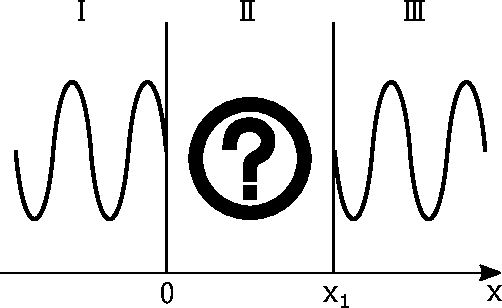
\includegraphics[height=3cm]{matrix/question.pdf}
\end{figure}
以下では簡単のために粒子のスピンを$1/2$とする。3つの領域I,II,IIIからなる系を考える。まず領域Iから波数$k$のスピン上向きの平面波
\begin{equation}
\psi^{\mathrm{inc}}=\begin{pmatrix} 1\\0 \end{pmatrix} \e^{ikx-i\omega_+ t}
\end{equation}
を入射する。Shr$\ddot{\mathrm{o}}$dinger方程式を系の境界条件のもとで解いて、領域IIIでの透過波が
\begin{equation}
\psi^{\mathrm{trans}}=\begin{pmatrix} a\e^{-i\omega_1t} \\ b\e^{-i\omega_2t} \end{pmatrix} \e^{ikx-i\omega_+ t}
\end{equation}
と求まったとする。ここで係数$a,b$やエネルギー変化$\omega_1,\omega_2$は入射波数と系の性質のみによってきまる定数とする。このときエネルギーは変わってもよいが、波数は変化していないことがポイントとなる。次に波数$k$のスピン下向き平面波
\begin{equation}
\psi^{\mathrm{inc}}=\begin{pmatrix} 0\\1 \end{pmatrix} \e^{ikx-i\omega_- t}
\end{equation}
を入射し、同様にShr$\ddot{\mathrm{o}}$dinger方程式を解いて領域IIIでの透過波が
\begin{equation}
\psi^{\mathrm{trans}}=\begin{pmatrix} c\e^{-i\omega_3t} \\ d\e^{-i\omega_4t} \end{pmatrix} \e^{ikx-i\omega_- t}
\end{equation}
と求まったとする。$c,d,\omega_3,\omega_4$も$a,b,\omega_1,\omega_2$と同様、入射波数と系の性質のみによってきまる定数とする。このときも波数は変化していない。すると、波数$k$の任意のスピン状態
\begin{equation}
\psi^{\mathrm{inc}}=\begin{pmatrix} p\e^{-i\omega_+t} \\ q\e^{-i\omega_-t}\end{pmatrix} \e^{ikx}
\end{equation}
を入射したときの領域IIIにおける透過波は、Shr$\ddot{\mathrm{o}}$dinger方程式の線形性から
\begin{equation}
\psi^{\mathrm{trans}}=\begin{pmatrix} a\e^{-i\omega_1t} & c\e^{-i\omega_3t} \\ b\e^{-i\omega_2t} & d\e^{-i\omega_4t} \end{pmatrix} \begin{pmatrix} p\e^{-i\omega_+t} \\ q\e^{-i\omega_-t}\end{pmatrix} \e^{ikx}
\end{equation}
となる。この結果は次のような見方ができる。すなわち波動関数を空間成分$K(x)$と時間・スピン成分$\chi(t)$に分けたとき、入射波と透過波で空間成分は変化せず
\begin{equation}
K^\mathrm{trans}(x)=K^\mathrm{inc}(x)=\e^{ikx}
\end{equation}
時間・スピン成分は変化しない入射波数と系の性質のみによって決まる行列$M(t)$を用いて
\begin{equation}
\chi^\mathrm{trans}(t)=M(t) \chi^\mathrm{inc}(t)
\end{equation}
と変換される。このような見方を行列形式と呼ぶことにする。上の例では
\begin{equation}
M(t)=\begin{pmatrix} a\e^{-i\omega_1t} & c\e^{-i\omega_3t} \\ b\e^{-i\omega_2t} & d\e^{-i\omega_4t} \end{pmatrix}
\end{equation}
である。ここで行列$M(t)$が時間のみに依存し、空間に依存しないことが重要な意味をもつ。

\paragraph{空間的な切り離し}
今度は7つの領域I,II,III,IV,V,VI,VIIからなる系を考える。ここで奇数番目の領域(I,III,V,VII)は全て同一の性質Oをもち、領域IIは性質Aを、領域IVは性質Bを、領域VIは性質Cをもつとする。さらに領域II、領域IV、領域VIの前後では波数が変化しないことが分かっている。
\begin{figure}[H]
\centering
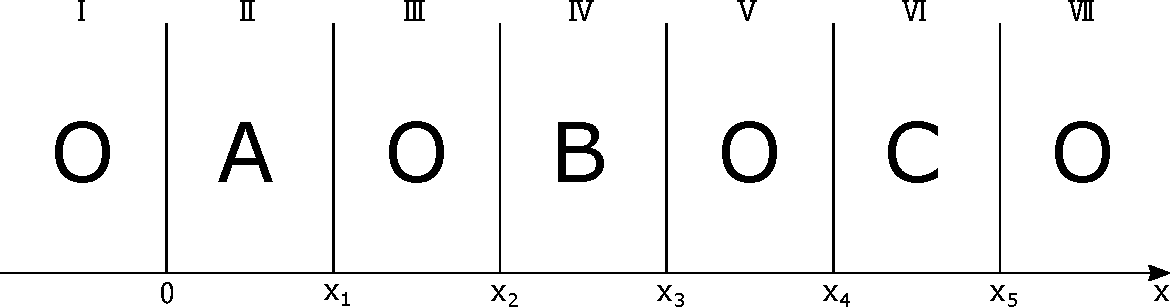
\includegraphics[height=3cm]{matrix/OABC.pdf}
\end{figure}
さて領域Iからスピン上向き平面波
\begin{equation}
\psi=\begin{pmatrix} 1\\0 \end{pmatrix} \e^{ik_+x-i\omega_0 t}
\end{equation}
を入射したとき領域VIIでの透過波はどのように表されるだろうか。もちろんShr$\ddot{\mathrm{o}}$dinger方程式を系の境界条件のもとで地道に解いてもよいが、ここでは前述の行列形式を用いよう。すなわち透過波を空間成分$K^\mathrm{trans}(x)$と時間・スピン成分$\chi^\mathrm{trans}(t)$に分け、性質A,B,Cから個別に求めた変換行列をそれぞれ$A(t),B(t),C(t)$とすると、
\begin{align}
&K^\mathrm{trans}=\e^{ik_+x} \\
&\chi^\mathrm{trans}=C(t)B(t)A(t) \begin{pmatrix} 1\\0 \end{pmatrix} \e^{-i\omega_0t}
\end{align}
と求まる。

ここで領域IIとIVの性質を入れ替える。つまり領域IIが性質Bを、領域IVが性質Aをもつとする。このとき先程と同様に領域Iからスピン上向き平面波を入射したときの領域VIIにおける透過波はどのように表されるか。Shr$\ddot{\mathrm{o}}$dinger方程式を解くとするとまた一から考える必要があるが、行列形式では変換行列が空間的な並びには依存しないことから
\begin{align}
&K^\mathrm{trans}=\e^{ik_+x} \\
&\chi^\mathrm{trans}=C(t)A(t)B(t) \begin{pmatrix} 1\\0 \end{pmatrix} \e^{-i\omega_0t}
\end{align}
とすぐに求まる。

このように行列形式の本質は領域の前後で波数が変わらないことを利用して、波動関数を空間的に形が変化しない空間成分と変化する時間・スピン成分に分けるところにある。それによって波動関数から空間的なつながりを切り離し、それぞれの領域を個別に考えた後で、好きな順番に並べ替えて議論することができる。

以下では具体的にそれぞれの装置の変換行列を求め、その後共鳴条件が満たされた場合のスピン干渉の式(\ref{theoretical})を再導出する。

\subsection{位相シフタコイル}
一様磁場中に位相シフタコイルがひとつ置かれた状況を考える。系は3つの領域I,II,IIIからなり、全体に$z$方向一様磁場$B_z$がかけられ、それに加えて領域IIに$z$方向一様磁場$B$がかけられている。
\begin{figure}[H]
\centering
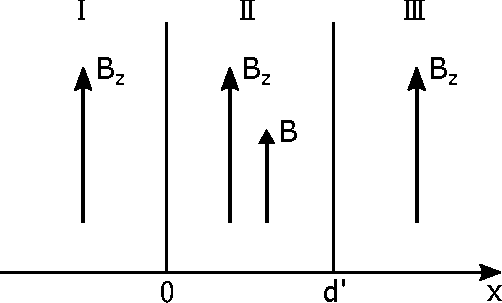
\includegraphics[height=3cm]{matrix/phaseshifter.pdf}
\end{figure}

\paragraph{領域I}
スピンの量子化軸を$z$軸に選ぶと、領域IにおけるShr$\ddot{\mathrm{o}}$dinger方程式は%なぜか\''{o}が使えない
\begin{equation}
i\frac{\del \psi_\mathrm{I}}{\del t}= \Biggl[-\frac{1}{2m} \frac{\del^2}{\del x^2} \underbrace{-\mu_nB_z}_{+|\mu_n|Bz =\omega_z} \sigma_z\Biggr] \psi_\mathrm{I}
\end{equation}
である。入射波数を$k$として、スピン上向き、下向きの入射波をそれぞれ
\begin{align}
\psi_\mathrm{I}=\begin{pmatrix} 1\\0 \end{pmatrix} \e^{i k x -i\omega_0 t} && \psi_\mathrm{I}=\begin{pmatrix} 0\\1 \end{pmatrix} \e^{i k x -i\omega^- t}
\end{align}
とすると
\begin{align}
&k=\sqrt{2m(\omega_0-\omega_z)} \\
&\omega^-=\frac{k^2}{2m} -\omega_z=\omega_0-2\omega_z
\end{align}
を得る。以後、入射エネルギーは外部磁場によるポテンシャルに比べて十分大きいとして近似し、全ての境界で反射を無視する。すなわち領域Iにおける波動関数は
\begin{align}
\psi_\mathrm{I}\simeq \begin{pmatrix} 1\\0 \end{pmatrix} \e^{i (k_0-\frac{\omega_z}{v}) x -i\omega_0 t} && \psi'_\mathrm{I}\simeq \begin{pmatrix} 0\\1 \end{pmatrix} \e^{i (k_0-\frac{\omega_z}{v}) x -i(\omega_0-2\omega_z) t}
\end{align}
と書ける。ここで$k_0 \equiv \sqrt{2m\omega_0},v \equiv k_0/m$とした。

\paragraph{領域II}
領域IIにおけるShr$\ddot{\mathrm{o}}$dinger方程式は
\begin{equation}
i\frac{\del \psi_\mathrm{II}}{\del t}= \left[-\frac{1}{2m} \frac{\del^2}{\del x^2} +(\omega_z+\omega) \sigma_z\right] \psi_\mathrm{II}
\end{equation}
ここで$\omega=|\mu_n|B$とした。領域IとIIの境界でエネルギーは変化しないので、領域IIにおけるスピン上下成分の波数$k^\pm_\mathrm{II}$は
\begin{align}
k^+_\mathrm{II}&=\sqrt{2m(\omega_0-(\omega_z+\omega))}\simeq k_0 -\frac{\omega_z}{v}-\frac{\omega}{v}\\
k^-_\mathrm{II}&=\sqrt{2m(\omega_0-2\omega_z+(\omega_z+\omega))}\simeq k_0 -\frac{\omega_z}{v}+\frac{\omega}{v}
\end{align}
となる。反射波を無視し、領域IとIIの境界(x=0)でそれぞれの入射波に対して波動関数を接続すると
\begin{align}
\psi_\mathrm{II}=\begin{pmatrix} 1\\0 \end{pmatrix} \e^{i (k_0-\frac{\omega_z}{v}-\frac{\omega}{v})x -i\omega_0 t} && \psi_\mathrm{II}=\begin{pmatrix} 0\\1 \end{pmatrix} \e^{i (k_0-\frac{\omega_z}{v} +\frac{\omega}{v}) x -i(\omega_0-2\omega_z) t}
\end{align}
を得る。

\paragraph{領域III}
領域IIIにおけるShr$\ddot{\mathrm{o}}$dinger方程式は領域Iと同じく
\begin{equation}
i\frac{\del \psi_\mathrm{I}}{\del t}= \Biggl[-\frac{1}{2m} \frac{\del^2}{\del x^2} +\omega_z \sigma_z\Biggr] \psi_\mathrm{I}
\end{equation}
である。領域IIとIIIの境界でエネルギーは変化しないので、領域IIIにおけるスピン上下成分の波数$k^\pm_\mathrm{III}$は
\begin{align}
k^+_\mathrm{III}=\sqrt{2m(\omega_0-\omega_z)}\simeq k_0 -\frac{\omega_z}{v}\\
k^-_\mathrm{III}=\sqrt{2m(\omega_0-2\omega_z+\omega_z)}\simeq k_0 -\frac{\omega_z}{v}
\end{align}
となる。領域IIとIIIの境界(x=d')でそれぞれの入射波に対して波動関数を接続すると
\begin{align}
\psi_\mathrm{III}=\begin{pmatrix} 1\\0 \end{pmatrix} \e^{-i\frac{\omega}{v}d'} \e^{i (k_0-\frac{\omega_z}{v})x -i\omega_0 t} && \psi_\mathrm{III}=\begin{pmatrix} 0\\1 \end{pmatrix} \e^{i\frac{\omega}{v}d} \e^{i (k_0-\frac{\omega_z}{v}) x -i(\omega_0-2\omega_z) t}
\end{align}
を得る。

\paragraph{変換行列}
以上より位相シフタコイルにおいて入射波と透過波の関係が次のように得られた:
\begin{align}
\psi_\mathrm{I}&= \begin{pmatrix} 1\\0 \end{pmatrix} \e^{i (k_0-\frac{\omega_z}{v}) x -i\omega_0 t} & \psi'_\mathrm{I}&= \begin{pmatrix} 0\\1 \end{pmatrix} \e^{i (k_0-\frac{\omega_z}{v}) x -i(\omega_0-2\omega_z) t} \\
\psi_\mathrm{III}&=\begin{pmatrix} 1\\0 \end{pmatrix} \e^{-i\frac{\omega}{v}d'} \e^{i (k_0-\frac{\omega_z}{v})x -i\omega_0 t} & \psi_\mathrm{III}&=\begin{pmatrix} 0\\1 \end{pmatrix} \e^{i\frac{\omega}{v}d} \e^{i (k_0-\frac{\omega_z}{v}) x -i(\omega_0-2\omega_z) t}
\end{align}
入射波と透過波を見比べることにより、位相シフタコイルの前後で波数は変化しないことが分かり、位相シフタコイルを表す変換行列$S$は
\begin{equation}
S=\begin{pmatrix} \e^{-i\frac{\omega}{v}d'} & 0\\0 &\e^{i\frac{\omega}{v}d'} \end{pmatrix}
\end{equation}
と求まる。

\subsection{共鳴スピンフリッパー}
一様磁場中に理想化されたRFスピンフリッパーがひとつ置かれた状況を考える。系は3つの領域I,II,IIIからなり、全体に$z$方向一様磁場$B_z$が、領域IIに$x$方向振動磁場$2B_r \cos \omega_s t$がかけられている。さらに以下では共鳴条件$\omega_s/2-\omega_z=0$が満たされている場合を扱う。
\begin{figure}[H]
\centering
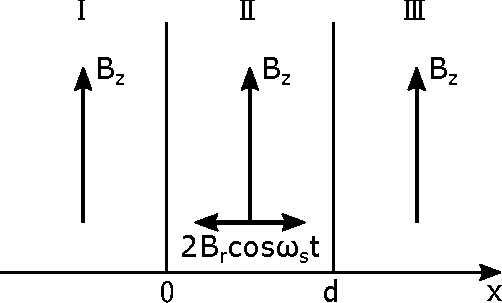
\includegraphics[height=3cm]{matrix/spinflipper.pdf}
\end{figure}

\paragraph{領域I}
領域Iは位相シフタコイルのときと全く同じで、波数$k$のスピン上向き、下向きの入射波はそれぞれ
\begin{align}
\psi_\mathrm{I}\simeq \begin{pmatrix} 1\\0 \end{pmatrix} \e^{i (k_0-\frac{\omega_z}{v}) x -i\omega_0 t} && \psi_\mathrm{I}\simeq \begin{pmatrix} 0\\1 \end{pmatrix} \e^{i (k_0-\frac{\omega_z}{v}) x -i(\omega_0-2\omega_z) t}
\end{align}
と表せる。

\paragraph{領域II}
\ref{pi2flipper_sec}章より領域IIにおける波動関数は反射波を無視すると一般に
\begin{equation}
\psi_\mathrm{II}=\begin{pmatrix} \left(A_n^+ \e^{ik_n^+x} -A_n^-\e^{ik_n^-x}\right)\e^{-i(\omega_n+\omega_z)} \\ \left(A_n^+ \e^{ik_n^+x} +A_n^-\e^{ik_n^-x} \right)\e^{-i(\omega_n-\omega_z)}\end{pmatrix}
\end{equation}
と書ける。ここで$k_n^\pm=\sqrt{2m(\omega_n\mp\omega_r)}$。よって$\psi_\mathrm{I}$と$\psi_\mathrm{II}$が領域IとIIの境界(x=0)において任意の時刻$t$で接続するためには
\begin{equation}
\omega_n=\omega_1\equiv \omega_0-\omega_z
\end{equation}
が必要である。そのとき
\begin{equation}
\psi_\mathrm{II}=\begin{pmatrix} \left(A_1^+ \e^{i(k_0-\frac{\omega_z}{v}-\frac{\omega_r}{v})x} -A_1^-\e^{i(k_0-\frac{\omega_z}{v}+\frac{\omega_r}{v})x}\right)\e^{-i\omega_0t} \\ \left(A_1^+ \e^{i(k_0-\frac{\omega_z}{v}-\frac{\omega_r}{v})x} +A_1^-\e^{i(k_0-\frac{\omega_z}{v}+\frac{\omega_r}{v})x}\right)\e^{-i(\omega_0-2\omega_z)t}\end{pmatrix}
\end{equation}
となる。領域IとIIの接続を考えると、スピン上向き、下向きの入射波に対してそれぞれ
\begin{align}
&\begin{cases}A_1^+-A_1^-=1\\A_1^++A_1^-=0\end{cases} &&\begin{cases}A_1^++A_1^-=1\\A_1^+-A_1^-=0\end{cases} \notag \\
&\Rightarrow \begin{cases} A_1^+=\frac{1}{2} \\ A_1^-=-\frac{1}{2}\end{cases} &&\Rightarrow \begin{cases} A_1^+=\frac{1}{2} \\ A_1^-=\frac{1}{2}\end{cases}
\end{align}
がなりたつ。したがってそれぞれの入射波に対する領域IIの波動関数は
\begin{align}
\psi_\mathrm{II} &=\begin{pmatrix} \frac{1}{2} \left(\e^{i(k_0-\frac{\omega_z}{v}-\frac{\omega_r}{v})x}+\e^{i(k_0-\frac{\omega_z}{v}+\frac{\omega_r}{v})x}\right) \e^{-i\omega_0t} \\ \frac{1}{2} \left(\e^{i(k_0-\frac{\omega_z}{v}-\frac{\omega_r}{v})x}-\e^{i(k_0-\frac{\omega_z}{v}+\frac{\omega_r}{v}x}\right) \e^{-i(\omega_0-2\omega_z)t}\end{pmatrix} &\psi_\mathrm{II}&=\begin{pmatrix} \frac{1}{2} \left(\e^{i(k_0-\frac{\omega_z}{v}-\frac{\omega_r}{v})x}-\e^{i(k_0-\frac{\omega_z}{v}+\frac{\omega_r}{v})x}\right) \e^{-i\omega_0t} \\ \frac{1}{2} \left(\e^{i(k_0-\frac{\omega_z}{v}-\frac{\omega_r}{v})x}+\e^{i(k_0-\frac{\omega_z}{v}+\frac{\omega_r}{v}x}\right) \e^{-i(\omega_0-2\omega_z)t}\end{pmatrix} \notag \\
&=\begin{pmatrix} \cos \frac{\omega_r x}{v} \e^{i(k_0-\frac{\omega_z}{v})x}\e^{-\omega_0t} \\ -i\sin\frac{\omega_r x}{v} \e^{i(k_0-\frac{\omega_z}{v})x}\e^{-i(\omega_0-2\omega_z)t} \end{pmatrix} &&=\begin{pmatrix} -i\sin\frac{\omega_rx}{v} \e^{i(k_0-\frac{\omega_z}{v})x}\e^{-\omega_0t} \\ \cos \frac{\omega_r x}{v} \e^{i(k_0-\frac{\omega_z}{v})x}\e^{-i(\omega_0-2\omega_z)t} \end{pmatrix}
\end{align}
となる。

\paragraph{領域III}
領域IIIも位相シフタコイルのときと同様にして、領域IIIにおけるスピン上下成分の波数$k^\pm_\mathrm{III}$は
\begin{align}
k^+_\mathrm{III}=\sqrt{2m(\omega_0-\omega_z)}\simeq k_0 -\frac{\omega_z}{v}\\
k^-_\mathrm{III}=\sqrt{2m(\omega_0-2\omega_z+\omega_z)}\simeq k_0 -\frac{\omega_z}{v}
\end{align}
となる。領域IIとIIIの境界(x=d)でそれぞれの入射波に対して波動関数を接続すると
\begin{align}
\psi_\mathrm{III}=\begin{pmatrix} \cos \frac{\omega_r d}{v} \e^{i(k_0-\frac{\omega_z}{v})x}\e^{-\omega_0t} \\ -i\sin\frac{\omega_r d}{v} \e^{i(k_0-\frac{\omega_z}{v})x}\e^{-i(\omega_0-2\omega_z)t} \end{pmatrix} &&\psi_\mathrm{III}=\begin{pmatrix} -i\sin\frac{\omega_rd}{v} \e^{i(k_0-\frac{\omega_z}{v})x}\e^{-\omega_0t} \\ \cos \frac{\omega_r x}{v} \e^{i(k_0-\frac{\omega_z}{v})d}\e^{-i(\omega_0-2\omega_z)t} \end{pmatrix}
\end{align}
を得る。

\paragraph{変換行列}
以上より共鳴条件を満たしたスピンフリッパーにおいて入射波と透過波の関係が次のように得られた:
\begin{align}
\psi_\mathrm{I}&= \begin{pmatrix} 1\\0 \end{pmatrix} \e^{i (k_0-\frac{\omega_z}{v}) x -i\omega_0 t} &\psi_\mathrm{I}&= \begin{pmatrix} 0\\1 \end{pmatrix} \e^{i (k_0-\frac{\omega_z}{v}) x -i(\omega_0-2\omega_z) t}\\
\psi_\mathrm{III}&=\begin{pmatrix} \cos \frac{\omega_r d}{v} \e^{i(k_0-\frac{\omega_z}{v})x}\e^{-\omega_0t} \\ -i\sin\frac{\omega_r d}{v} \e^{i(k_0-\frac{\omega_z}{v})x}\e^{-i(\omega_0-2\omega_z)t} \end{pmatrix} &\psi_\mathrm{III}&=\begin{pmatrix} -i\sin\frac{\omega_rd}{v} \e^{i(k_0-\frac{\omega_z}{v})x}\e^{-\omega_0t} \\ \cos \frac{\omega_r d}{v} \e^{i(k_0-\frac{\omega_z}{v})x}\e^{-i(\omega_0-2\omega_z)t} \end{pmatrix}
\end{align}
入射波と透過波を見比べることにより、共鳴スピンフリッパーの前後で波数は変化しないことが分かり、共鳴スピンフリッパーを表す変換行列$F$は
\begin{equation}
F=\begin{pmatrix} \cos \frac{\omega_r d}{v} &-i\sin\frac{\omega_rd}{v}\e^{-2i\omega_zt} \\ -i\sin\frac{\omega_rd}{v}\e^{+2i\omega_zt} &\cos \frac{\omega_r d}{v}\end{pmatrix}
\end{equation}
と求まる。

\subsection{スピン干渉}
いよいよ行列形式でスピン干渉を見てゆく。一様磁場中にスピンフリッパー、位相シフタコイル、スピンフリッパーが順番に置かれた状況を考える。系は7つの領域I,II,III,IV,V,VI,VIIからなり、全体に$z$方向一様磁場$B_z$がかけられ、それに加えて領域II,VIに$x$方向振動磁場$2B_r\cos\omega_s t$が、領域IVに$z$方向一様磁場$B$がかけられている。
\begin{figure}[H]
\centering
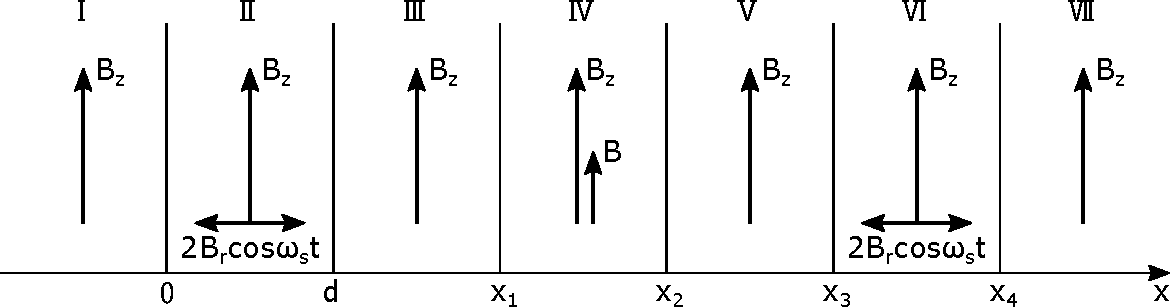
\includegraphics[height=3cm]{matrix/interference.pdf}
\end{figure}

領域Iからスピン上向き平面波
\begin{equation}
\psi_\mathrm{I}(x,t)=\underbrace{\begin{pmatrix} 1\\0\end{pmatrix} \e^{-i\omega_0t}}_{\chi_\mathrm{I}(t)} \underbrace{\e^{i (k_0-\frac{\omega_z}{v})x}}_{K_\mathrm{I}(x)}
\end{equation}
を入射したとき、領域VIIにおける波動関数$\psi_\mathrm{VII}(x,t)$の空間成分$K_\mathrm{VII}(x)$と時間・スピン成分$\chi_\mathrm{VII}(t)$は
\begin{align}
K_\mathrm{VII}(x)=K_\mathrm{I}(x)=\e^{i (k_0-\frac{\omega_z}{v})x}
\end{align}
\begin{align}
\chi_\mathrm{VII}(t)&=FSF\chi_\mathrm{I}(t) \notag \\
&=\scalebox{0.9}{$\begin{pmatrix} \cos \frac{\omega_r d}{v} &-i\sin\frac{\omega_rd}{v}\e^{-2i\omega_zt} \\ -i\sin\frac{\omega_rd}{v}\e^{+2i\omega_zt} &\cos \frac{\omega_r d}{v}\end{pmatrix}\begin{pmatrix} \e^{-i\frac{\omega}{v}d'} & 0\\0 &\e^{i\frac{\omega}{v}d'} \end{pmatrix}\begin{pmatrix} \cos \frac{\omega_r d}{v} &-i\sin\frac{\omega_rd}{v}\e^{-2i\omega_zt} \\ -i\sin\frac{\omega_rd}{v}\e^{+2i\omega_zt} &\cos \frac{\omega_r d}{v}\end{pmatrix} \begin{pmatrix} 1\\0\end{pmatrix} \e^{-i\omega_0t}$} \notag \\
&=\begin{pmatrix} \cos^2 \frac{\omega_r d}{v} \e^{-i\frac{\omega d'}{v}} -\sin^2 \frac{\omega_r d}{v} \e^{i\frac{\omega d'}{v}} \\ -i\sin\frac{\omega_r d}{v}\cos\frac{\omega_r d}{v}\left(\e^{-i\frac{\omega d'}{v}}+\e^{i\frac{\omega d'}{v}} \right) \e^{i\omega_s t} \end{pmatrix}\e^{-i\omega_0t}
\end{align}
となる。したがって領域VIIにおいてスピン上向き中性子を観測する確率は
\begin{align}
|\psi_\mathrm{VII}^+|^2&=|\chi_\mathrm{VII}^+|^2=\Biggl|\cos^2 \frac{\omega_r d}{v} \e^{-i\frac{\omega d'}{v}} -\sin^2 \frac{\omega_r d}{v} \e^{i\frac{\omega d'}{v}}\Biggr|^2\notag \\
&=\cos^4 \frac{\omega_r d}{v} +\sin^4 \frac{\omega_r d'}{v} -2\sin^2\frac{\omega_rd}{v}\cos^2\frac{\omega_rd}{v} \cos \frac{2\omega d'}{v} \notag \\
&=1-\sin^2 \frac{2\omega_r d}{v} \cos^2 \frac{\omega d'}{v}
\end{align}
となる。確かに\ref{pi2flipper_sec}章の最後に得られた結果が再び導出された。
\renewcommand{\arraystretch}{1}






\section{必ずしも共鳴条件を満たさない場合}\label{nonreso_sec}
これまではシンプルにスピン干渉という現象を見るために、共鳴条件(\ref{pi2flipper_resonance})が満たされる場合のみを扱ってきた。しかし、実際の解析では共鳴条件を満たさない場合も扱う必要があるため、この章ではより一般的に必ずしも共鳴条件を満たさない場合に何が起こるかを見てゆく。


\subsection{スピンフリッパーの機能}
スピン干渉について考える前に、共鳴条件を満たさない場合のスピンフリッパーの機能について考えよう。

\paragraph{舞台とあらすじ}
一様磁場中に理想化されたRFスピンフリッパーがひとつ置かれた状況を考える。系は3つの領域I,II,IIIからなり、全体に$z$方向一様磁場$B_z$が、領域IIに$x$方向振動磁場$2B_r \cos \omega_s t$がかけられている。
\begin{figure}[h]
\centering
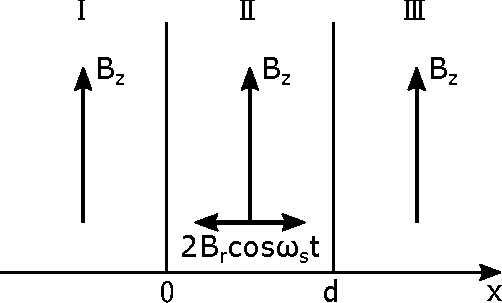
\includegraphics[height=3cm]{nonreso/resonance_setting1.pdf}
\end{figure}

これから述べるように、スピン上向きの中性子が領域Iから速度$v$で入射し領域IIを通って領域IIIに抜けるとき、領域IIIにおけるスピン上向き中性子の存在確率は
\begin{equation}
|\psi_{\mathrm{III}}^+|^2=\cos^2 \frac{\omega_A}{v}d+\left(\frac{\epsilon}{\omega_A}\right)^2\sin^2\frac{\omega_A}{v}d \label{Nonreso_flip}
\end{equation}
となる。ここで$\epsilon=\omega_s/2-\omega_z,\omega_A=\sqrt{\epsilon^2+\omega_r^2}$であり、$\omega_z=|\mu_n|B_z,\omega_r=|\mu_n|B_r$、$\mu_n$は中性子の磁気モーメント、$d$は領域IIの幅である。ここで定義した
\begin{equation}
\epsilon=\frac{\omega_s}{2}-\omega_z
\end{equation}
という量は共鳴からのずれを表す指標であり、この章で非常に重要な役割を演じる。

\begin{comment}
式(\ref{Nonreso_flip})を見ると$\epsilon=0$がなりたてば、$\omega_rd/v=\pi/2$を満たす速度の中性子に対して、領域IIIにおけるスピン上向き粒子の存在確率が0、すなわちスピン反転率が1になることがわかる。逆に$\epsilon \neq 0$のときはどのような速度の中性子に対しても反転率は1となり得ない。このように、$\epsilon=0$を満たす周波数の振動磁場をかけたときに限りスピンフリッパーを通り抜けた中性子のスピンが完全に反転し得る。これをスピンフリッパーの共鳴と呼び、$\epsilon=0$を共鳴条件と呼んだのであった。
\end{comment}

\renewcommand{\arraystretch}{1.5}

\paragraph{入射波}
スピンの量子化軸を$z$軸に選ぶと、領域IにおけるShr$\ddot{\mathrm{o}}$dinger方程式は%なぜか\''{o}が使えない
\begin{equation}
i\frac{\del \psi_\mathrm{I}}{\del t}= \Biggl[-\frac{1}{2m} \frac{\del^2}{\del x^2} \underbrace{-\mu_nB_z}_{+|\mu_n|Bz =\omega_z} \sigma_z\Biggr] \psi_\mathrm{I}
\end{equation}
入射中性子のスピンは上向きとしたので、そのエネルギーを$\omega_0$とすると、領域Iにおける波動関数の入射成分はスピン上下の2成分表示で
\begin{equation}
\psi_\mathrm{I}^{\mathrm{in}}=\begin{pmatrix} 1\\0 \end{pmatrix} \e^{i k_0^+ x -i\omega_0 t}
\end{equation}
と書ける。ここで$k_0^+=\sqrt{2m(\omega_0 -\omega_z)}$。
\renewcommand{\arraystretch}{1}

\paragraph{領域II}
領域IIにおける磁場を
\begin{equation}
\bm{B}_{\mathrm{II}}=\hat{\bm{x}} (2B_r)\cos \omega_s t+\hat{\bm{z}} B_z
\end{equation}
と書く。ただし$\hat{\bm{x}},\hat{\bm{z}}$はそれぞれx,z軸正の向きの単位ベクトル。$|B_r| \ll |B_z|$のときには、\ref{pi2flipper_sec}章で述べた理由により振動磁場を次のような$xy$平面上の回転磁場に置き換えてよい:
\begin{equation}
\hat{\bm{x}} (2B_r)\cos \omega_s t \rightarrow \hat{\bm{x}} B_r \cos \omega_s t+\hat{\bm{y}} \sin \omega_s t
\end{equation}
したがって$|B_r| \ll |B_z|$のとき領域IIにおける磁場は
\begin{equation}
\bm{B}_{\mathrm{II}}\simeq \hat{\bm{x}} B_r\cos \omega_s t+\hat{\bm{y}} B_r \sin \omega_s t+\hat{\bm{z}} B_z
\end{equation}
となる。このとき領域IIにおけるShr$\ddot{\mathrm{o}}$dinger方程式は
\begin{align}
i\frac{\del \psi_{\mathrm{II}}}{\del t} &=\left[-\frac{1}{2m} \frac{\del^2}{\del x^2} -\bm{\mu}_n\cdot\bm{B}_\mathrm{II}\right] \psi_\mathrm{II}\notag \\
&=\left[-\frac{1}{2m} \frac{\del^2}{\del x^2} + |\mu_n| (\sigma_x B_r \cos\omega_s t+\sigma_y B_r\sin\omega_s t+\sigma_zB_z)\right] \psi_\mathrm{II} \notag \\
&=\left[-\frac{1}{2m} \frac{\del^2}{\del x^2} +\begin{pmatrix} \omega_z &\omega_r \e^{-i\omega_s t} \\\omega_r \e^{i\omega_s t} &-\omega_z \end{pmatrix}\right] \psi_\mathrm{II}
\end{align}
となる。まずハミルトニアンの時間依存性を除くために、$z$軸まわりの角速度$-\omega_s$の回転を表すユニタリ変換
\begin{equation}
U_T=\exp\left[+iS_z\omega_s t\right] =\exp\left[i\sigma_z\frac{\omega_s t}{2}\right]=\begin{pmatrix} \e^{i\omega_st/2} &0\\0&\e^{-i\omega_st/2}\end{pmatrix}
\end{equation}
を用いて
\begin{equation}
U_T \begin{pmatrix} \omega_z &\omega_r \e^{-i\omega_s t} \\\omega_r \e^{i\omega_s t} &-\omega_z \end{pmatrix} U_T^\dagger =\begin{pmatrix} \omega_z &\omega_r\\ \omega_r&-\omega_z \end{pmatrix}
\end{equation}
がなりたつことに注意すると、
\begin{equation}
i\frac{\del}{\del t}(U_T \psi_\mathrm{II}) =\left[-\frac{1}{2m} \frac{\del^2}{\del x^2} +\begin{pmatrix} -(\frac{\omega_s}{2}-\omega_z) &\omega_r\\ \omega_r &\frac{\omega_s}{2}-\omega_z \end{pmatrix}\right] (U_T \psi_\mathrm{II})
\end{equation}
を得る。さらにこのハミルトニアンを対角的にするために
\begin{equation}
\begin{pmatrix} -(\frac{\omega_s}{2}-\omega_z) &\omega_r\\ \omega_r &\frac{\omega_s}{2}-\omega_z \end{pmatrix}=\omega_A\begin{pmatrix} \cos \theta&\sin \theta\\ \sin \theta &-\cos \theta \end{pmatrix}
\end{equation}
と書く。ここで$\epsilon=\omega_s/2-\omega_z,\omega_A=\sqrt{\epsilon^2+\omega_r^2}$として
\begin{equation}
\cos \theta=\frac{-\epsilon}{\omega_A} , \quad \sin \theta=\frac{\omega_r}{\omega_A}
\end{equation}
である。$y$軸まわりの角度$-\theta$回転を表すユニタリ変換
\begin{equation}
U_D=\exp\left[+iS_y \theta\right] =\exp\left[i\sigma_y \frac{\theta}{2}\right] =\begin{pmatrix} \cos\frac{\theta}{2}& \sin\frac{\theta}{2}\\  -\sin\frac{\theta}{2}& \cos\frac{\theta}{2}\end{pmatrix}
\end{equation}
を用いて
\begin{equation}
U_D \begin{pmatrix} \cos \theta&\sin \theta\\ \sin \theta &-\cos \theta \end{pmatrix} U_D^\dagger =\begin{pmatrix} 1&0\\0&-1\end{pmatrix}
\end{equation}
がなりたつことに注意すると、
\begin{equation}
i\frac{\del}{\del t}(U_DU_T \psi_\mathrm{II}) =\left[-\frac{1}{2m} \frac{\del^2}{\del x^2} +\omega_A \sigma_Z \right] (U_DU_T \psi_\mathrm{II})
\end{equation}
を得る。

\renewcommand{\arraystretch}{1.5}
したがって、領域IIにおける中性子のエネルギーを$\omega_n$とすると、定数$A_n^\pm,B_n^\pm$を用いて
\begin{equation}
\psi_D \equiv U_D U_T \psi_\mathrm{II} =\begin{pmatrix} A_n^+ \e^{ik_n^+x}+B_n^+\e^{-ik_n^+x} \\ A_n^- \e^{ik_n^-x}+B_n^-\e^{-ik_n^-x} \end{pmatrix} \e^{-i\omega_n t}
\end{equation}
と書けるから、領域IIにおける波動関数は
\begin{align}
\psi_\mathrm{II}&=U_T^\dagger U_D^\dagger \psi_D \notag \\
&=\begin{pmatrix} \e^{-i\omega_st/2} &0\\0&\e^{+i\omega_st/2}\end{pmatrix} \begin{pmatrix} \cos\frac{\theta}{2}& -\sin\frac{\theta}{2}\\  \sin\frac{\theta}{2}& \cos\frac{\theta}{2}\end{pmatrix} \begin{pmatrix} A_n^+ \e^{ik_n^+x}+B_n^+\e^{-ik_n^+x} \\ A_n^- \e^{ik_n^-x}+B_n^-\e^{-ik_n^-x} \end{pmatrix} \e^{-i\omega_n t} \notag \\
&=\begin{pmatrix} \left(A_n^+ \cos \frac{\theta}{2} \e^{ik_n^+x}+ B_n^+ \cos \frac{\theta}{2} \e^{-ik_n^+x} - A_n^- \sin \frac{\theta}{2} \e^{ik_n^-x}- B_n^- \sin \frac{\theta}{2} \e^{-ik_n^-x}\right) \e^{-i(\omega_n+\omega_s/2)t} \\ \left(A_n^+ \sin \frac{\theta}{2} \e^{ik_n^+x}+ B_n^+ \sin \frac{\theta}{2} \e^{-ik_n^+x} + A_n^- \cos \frac{\theta}{2} \e^{ik_n^-x}+ B_n^- \cos \frac{\theta}{2} \e^{-ik_n^-x}\right) \e^{-i(\omega_n-\omega_s/2)t} \end{pmatrix} \label{Nonreso_psi2}
\end{align}
と書ける。ここで$k_n^\pm=\sqrt{2m(\omega_n \mp \omega_A)}$。

\paragraph{領域IとIIの接続}
入射波$\psi_\mathrm{I}^\mathrm{in}$と$\psi_\mathrm{II}$が任意の時刻$t$で領域IとIIの境界($x=0$)において接続するためには
\begin{equation}
\omega_n=\omega_1 \equiv \omega_0 -\frac{\omega_s}{2}
\end{equation}
が必要である。そのとき
\begin{equation}
\psi_\mathrm{II}=\begin{pmatrix} \left(A_1^+ \cos \frac{\theta}{2} \e^{ik_1^+x}+ B_1^+ \cos \frac{\theta}{2} \e^{-ik_1^+x} - A_1^- \sin \frac{\theta}{2} \e^{ik_1^-x}- B_1^- \sin \frac{\theta}{2} \e^{-ik_1^-x}\right) \e^{-i\omega_0t} \\ \left(A_1^+ \sin \frac{\theta}{2} \e^{ik_1^+x}+ B_1^+ \sin \frac{\theta}{2} \e^{-ik_1^+x} + A_1^- \cos \frac{\theta}{2} \e^{ik_1^-x}+ B_1^- \cos \frac{\theta}{2} \e^{-ik_1^-x}\right) \e^{-i(\omega_0-\omega_s)t} \end{pmatrix}
\end{equation}
ここで$k_1^\pm=\sqrt{2m(\omega_0-\omega_s/2 \mp \omega_A)}$。

またこのことから、領域Iでの反射波を含めた全波動関数$\psi_\mathrm{I}$は
\begin{equation}
\psi_\mathrm{I} =I_0^+ \psi_\mathrm{I}^\mathrm{in} +\begin{pmatrix} R_0^+ \e^{-ik_0^+x}\e^{ -i\omega_0 t} \\ R_2^- \e^{-ik_2^-x}\e^{ -i (\omega_0-\omega_s)t} \end{pmatrix} =\begin{pmatrix} (I_0^+ \e^{ik_0^+x} +R_0^+\e^{-ik_0^+x} )\e^{-i\omega_0 t} \\ R_2^- \e^{-ik_2^-x}\e^{ -i (\omega_0-\omega_s)t} \end{pmatrix}
\end{equation}
と書ける。ここで$I_0^+,R_0^+,R_2^-$は定数であり、$k_0^+ =\sqrt{2m(\omega_0 -\omega_z)},k_2^- =\sqrt{2m(\omega_0 -\omega_s +\omega_z)}$である。

さて、ここで領域IとIIの接続を考えると、次の4つの式がなりたつ:
\begin{align}
\left\{\begin{array}{l}
A_1^+ \cos \frac{\theta}{2} +B_1^+\cos \frac{\theta}{2} -A_1^-\sin\frac{\theta}{2} -B_1^-\sin\frac{\theta}{2} = I_0^+ +R_0^+ \\
k_1^+(A_1^+ \cos \frac{\theta}{2} -B_1^+\cos \frac{\theta}{2} )-k_1^-(A_1^-\sin\frac{\theta}{2} -B_1^-\sin\frac{\theta}{2} )=k_0^+(I_0^--R_0^+)\\
A_1^+ \sin \frac{\theta}{2} +B_1^+\sin \frac{\theta}{2} +A_1^-\cos\frac{\theta}{2} +B_1^-\cos\frac{\theta}{2} = R_2^- \\
k_1^+(A_1^+ \sin \frac{\theta}{2} -B_1^+\sin \frac{\theta}{2}) +k_1^-(A_1^-\cos\frac{\theta}{2} -B_1^-\cos\frac{\theta}{2}) = -k_2^-R_2^-
\end{array} \right. \label{Nonreso_setsuzoku}
\end{align}

\paragraph{近似}
いま中性子の入射エネルギー$\omega_0$は、$\omega_z$や$\omega_s,\omega_r$などと比べて十分大きいとする。このとき
\begin{align}
&k_0^+ =\sqrt{2m(\omega_0 -\omega_z)} \simeq k_0 -\frac{\omega_z}{v} \label{Nonreso_k0+} \\
&k_1^{\pm} = \sqrt{2m(\omega_0-\omega_s/2 \mp \omega_A)} \simeq k_0 -\frac{\omega_s}{2v} \mp \frac{\omega_A}{v} \label{Nonreso_k1+-} \\
&k_2^- =\sqrt{2m(\omega_0 -\omega_s +\omega_z)} \simeq k_0 -\frac{\omega_s}{v} +\frac{\omega_z}{v}\label{Nonreso_k2-}
\end{align}
となる。ここで$k_0 \equiv \sqrt{2m\omega_0}$とした。さらに式(\ref{Nonreso_setsuzoku})のように両辺で$k_0$が打ち消し合わないときは
\begin{equation}
k_n^\pm \simeq k_0\label{Nonreso_kn+-}
\end{equation}
と近似する。後で見るようにこれは反射波を無視することと同値である。

この近似の下で式(\ref{Nonreso_setsuzoku})は次のように変形される:
\begin{align}
&\left\{\begin{array}{l}
A_1^+ \cos \frac{\theta}{2} +B_1^+\cos \frac{\theta}{2} -A_1^-\sin\frac{\theta}{2} -B_1^-\sin\frac{\theta}{2} = I_0^+ +R_0^+ \\
k_0(A_1^+ \cos \frac{\theta}{2} -B_1^+\cos \frac{\theta}{2} )-k_0(A_1^-\sin\frac{\theta}{2} -B_1^-\sin\frac{\theta}{2} )=k_0(I_0^--R_0^+)\\
A_1^+ \sin \frac{\theta}{2} +B_1^+\sin \frac{\theta}{2} +A_1^-\cos\frac{\theta}{2} +B_1^-\cos\frac{\theta}{2} = R_2^- \\
k_0(A_1^+ \sin \frac{\theta}{2} -B_1^+\sin \frac{\theta}{2}) +k_0(A_1^-\cos\frac{\theta}{2} -B_1^-\cos\frac{\theta}{2}) = -k_0R_2^-
\end{array} \right.  \notag \\
&\Rightarrow \left\{\begin{array}{l}
A_1^+ \cos \frac{\theta}{2} +B_1^+\cos \frac{\theta}{2} -A_1^-\sin\frac{\theta}{2} -B_1^-\sin\frac{\theta}{2} = I_0^+ +R_0^+ \\
A_1^+ \cos \frac{\theta}{2} -B_1^+\cos \frac{\theta}{2} -A_1^-\sin\frac{\theta}{2} -B_1^-\sin\frac{\theta}{2} =I_0^--R_0^+\\
A_1^+ \sin \frac{\theta}{2} +B_1^+\sin \frac{\theta}{2} +A_1^-\cos\frac{\theta}{2} +B_1^-\cos\frac{\theta}{2} = R_2^- \\
A_1^+ \sin \frac{\theta}{2} -B_1^+\sin \frac{\theta}{2} +A_1^-\cos\frac{\theta}{2} -B_1^-\cos\frac{\theta}{2} = -R_2^-
\end{array} \right.  \notag \\
&\Rightarrow \left\{\begin{array}{l}
A_1^+ \cos \frac{\theta}{2} -A_1^-\sin\frac{\theta}{2}= I_0^+ \\
B_1^+\cos \frac{\theta}{2} -B_1^-\sin\frac{\theta}{2} =R_0^+\\
A_1^+ \sin \frac{\theta}{2}+A_1^-\cos\frac{\theta}{2}= 0 \\
B_1^+\sin \frac{\theta}{2} -B_1^-\cos\frac{\theta}{2} = R_2^-
\end{array} \right.  \notag \\
&\Rightarrow \left\{\begin{array}{l}
A_1^+ = I_0^+\cos\frac{\theta}{2} \\
A_1^- =-I_0^+\sin\frac{\theta}{2} \\
B_1^+=R_0^+\cos\frac{\theta}{2}+R_2^-\sin\frac{\theta}{2} \\
B_1^-=R_2^-\cos\frac{\theta}{2}-R_0\sin\frac{\theta}{2}
\end{array} \right. \label{Nonreso_1and2}
\end{align}

\paragraph{領域III}
領域IIIにおけるShr$\ddot{\mathrm{o}}$dinger方程式は領域Iと同じで
\begin{equation}
i\frac{\del \psi_\mathrm{III}}{\del t}= \left[-\frac{1}{2m} \frac{\del^2}{\del x^2} +\omega_z \sigma_z\right] \psi_\mathrm{III}
\end{equation}
である。$\psi_\mathrm{II}$と$\psi_\mathrm{III}$が任意の時刻$t$で領域IIとIIIの境界($x=d$)において接続するためには、式(\ref{Nonreso_psi2})より、領域IIIにおける中性子のエネルギーがスピン上向きに対しては$\omega_0$、スピン下向きに対しては$\omega_0-\omega_s$であることが必要である。よって領域IIIにおける波動関数$\psi_\mathrm{III}$は定数$C_0^+,C_2^-$を用いて
\begin{equation}
\psi_\mathrm{III}=\begin{pmatrix} C_0^+ \e^{ik_0^+ x}\e^{-i\omega_0 t} \\ C_2^- \e^{ik_2^- x}\e^{-i(\omega_0-\omega_s) t} \end{pmatrix}
\end{equation}
と書ける。ここで$k_0^+=\sqrt{2m(\omega_0-\omega_z)},k_2^-=\sqrt{2m(\omega_0-\omega_s+\omega_z)}$。

\paragraph{領域IIとIIIの接続}
次に領域IIとIIIの接続を考える。前述の通り、波数の内、両辺で$k_0$が打ち消しあいその差が現れるもの(指数の肩に乗っているもの)については式(\ref{Nonreso_k0+}),(\ref{Nonreso_k1+-}),(\ref{Nonreso_k2-})のように、両辺で$k_0$が打ち消し合わないもの(指数の肩から降りているもの)については式(\ref{Nonreso_kn+-})のように近似する。すると次の4つの式がなりたつ:
\begin{align}
&\left\{\begin{array}{l}
\left(A_1^+ \cos \frac{\theta}{2} \e^{-i\frac{\omega_A}{v}d}+B_1^+\cos \frac{\theta}{2} \e^{i\frac{\omega_A}{v}d}-A_1^-\sin\frac{\theta}{2}\e^{i\frac{\omega_A}{v}d} -B_1^-\sin\frac{\theta}{2}\e^{-i\frac{\omega_A}{v}d} \right)\e^{i(k_0-\frac{\omega_s}{2v})d}= C_0^+\e^{i(k_0-\frac{\omega_z}{v})d} \\
\left(A_1^+ \cos \frac{\theta}{2} \e^{-i\frac{\omega_A}{v}d}-B_1^+\cos \frac{\theta}{2} \e^{i\frac{\omega_A}{v}d}-A_1^-\sin\frac{\theta}{2}\e^{i\frac{\omega_A}{v}d} +B_1^-\sin\frac{\theta}{2}\e^{-i\frac{\omega_A}{v}d} \right)\e^{i(k_0-\frac{\omega_s}{2v})d}= C_0^+\e^{i(k_0-\frac{\omega_z}{v})d} \\
\left(A_1^+ \sin \frac{\theta}{2} \e^{-i\frac{\omega_A}{v}d}+B_1^+\sin \frac{\theta}{2} \e^{i\frac{\omega_A}{v}d}+A_1^-\cos\frac{\theta}{2}\e^{i\frac{\omega_A}{v}d} +B_1^-\cos\frac{\theta}{2}\e^{-i\frac{\omega_A}{v}d} \right)\e^{i(k_0-\frac{\omega_s}{2v})d}= C_2^-\e^{i(k_0-\frac{\omega_s}{v}+\frac{\omega_z}{v})d} \\
\left(A_1^+ \sin \frac{\theta}{2} \e^{-i\frac{\omega_A}{v}d}-B_1^+\sin \frac{\theta}{2} \e^{i\frac{\omega_A}{v}d}+A_1^-\cos\frac{\theta}{2}\e^{i\frac{\omega_A}{v}d} -B_1^-\cos\frac{\theta}{2}\e^{-i\frac{\omega_A}{v}d} \right)\e^{i(k_0-\frac{\omega_s}{2v})d}= C_2^-\e^{i(k_0-\frac{\omega_s}{v}+\frac{\omega_z}{v})d} \\
\end{array} \right.  \notag \\
&\Rightarrow \left\{\begin{array}{l}
\left(A_1^+ \cos \frac{\theta}{2} \e^{-i\frac{\omega_A}{v}d}+B_1^+\cos \frac{\theta}{2} \e^{i\frac{\omega_A}{v}d}-A_1^-\sin\frac{\theta}{2}\e^{i\frac{\omega_A}{v}d} -B_1^-\sin\frac{\theta}{2}\e^{-i\frac{\omega_A}{v}d} \right)\e^{-i\frac{\frac{\omega_s}{2}-\omega_z}{v}d}= C_0^+\\
\left(A_1^+ \cos \frac{\theta}{2} \e^{-i\frac{\omega_A}{v}d}-B_1^+\cos \frac{\theta}{2} \e^{i\frac{\omega_A}{v}d}-A_1^-\sin\frac{\theta}{2}\e^{i\frac{\omega_A}{v}d} +B_1^-\sin\frac{\theta}{2}\e^{-i\frac{\omega_A}{v}d} \right)\e^{-i\frac{\frac{\omega_s}{2}-\omega_z}{v}d}= C_0^+\\
\left(A_1^+ \sin \frac{\theta}{2} \e^{-i\frac{\omega_A}{v}d}+B_1^+\sin \frac{\theta}{2} \e^{i\frac{\omega_A}{v}d}+A_1^-\cos\frac{\theta}{2}\e^{i\frac{\omega_A}{v}d} +B_1^-\cos\frac{\theta}{2}\e^{-i\frac{\omega_A}{v}d} \right)\e^{i\frac{\frac{\omega_s}{2}-\omega_z}{v}d}= C_2^-\\
\left(A_1^+ \sin \frac{\theta}{2} \e^{-i\frac{\omega_A}{v}d}-B_1^+\sin \frac{\theta}{2} \e^{i\frac{\omega_A}{v}d}+A_1^-\cos\frac{\theta}{2}\e^{i\frac{\omega_A}{v}d} -B_1^-\cos\frac{\theta}{2}\e^{-i\frac{\omega_A}{v}d} \right)\e^{i\frac{\frac{\omega_s}{2}-\omega_z}{v}d}= C_2^- \\
\end{array} \right.  \notag \\
&\Rightarrow \left\{\begin{array}{l}
\left(A_1^+ \cos \frac{\theta}{2} \e^{-i\frac{\omega_A}{v}d}-A_1^-\sin\frac{\theta}{2}\e^{i\frac{\omega_A}{v}d} \right)\e^{-i\frac{\epsilon}{v} d}= C_0^+\\
\left(B_1^+\cos \frac{\theta}{2} \e^{i\frac{\omega_A}{v}d}-B_1^-\sin\frac{\theta}{2}\e^{-i\frac{\omega_A}{v}d} \right)\e^{-i\frac{\epsilon}{v} d}= 0\\
\left(A_1^+ \sin \frac{\theta}{2} \e^{-i\frac{\omega_A}{v}d}+A_1^-\cos\frac{\theta}{2}\e^{i\frac{\omega_A}{v}d} \right)\e^{i\frac{\epsilon}{v} d}= C_2^- \\
\left(B_1^+\sin \frac{\theta}{2} \e^{i\frac{\omega_A}{v}d}+B_1^-\cos\frac{\theta}{2}\e^{-i\frac{\omega_A}{v}d} \right)\e^{i\frac{\epsilon}{v} d}= 0
\end{array} \right. \notag \\
&\Rightarrow \left\{\begin{array}{l}
C_0^+=\left(A_1^+ \cos \frac{\theta}{2} \e^{-i\frac{\omega_A}{v}d}-A_1^-\sin\frac{\theta}{2}\e^{i\frac{\omega_A}{v}d} \right)\e^{-i\frac{\epsilon}{v} d}\\
C_2^-=\left(A_1^+ \sin \frac{\theta}{2} \e^{-i\frac{\omega_A}{v}d}+A_1^-\cos\frac{\theta}{2}\e^{i\frac{\omega_A}{v}d} \right)\e^{i\frac{\epsilon}{v} d}\\
B_1^+=0\\
B_1^-= 0
\end{array} \right. \label{Nonreso_2and3}
\end{align}
%ここで$\epsilon=\omega_s/2-\omega_z$とした。
%\end{comment}


\paragraph{結末}
したがって式(\ref{Nonreso_1and2}),(\ref{Nonreso_2and3})より
\begin{equation}
\left\{ \begin{array}{l}
A_1^+=I_0^+ \cos \frac{\theta}{2} \\
A_1^-=-I_0^+ \cos \frac{\theta}{2} \\
B_1^+=0 \\
B_1^-=0 \\
C_0^+=I_0^+\left(\sin^2 \frac{\theta}{2} \e^{i\frac{\omega_A}{v}d} +\cos^2 \frac{\theta}{2} \e^{-i\frac{\omega_A}{v}d} \right)  \e^{-i\frac{\epsilon}{v}d} \\
C_2^-=I_0^+ \sin\frac{\theta}{2}\cos\frac{\theta}{2} \left(\e^{-i\frac{\omega_A}{v}d}-\e^{i\frac{\omega_A}{v}d}\right) \e^{i\frac{\epsilon}{v}d}\\
R_0^+=0\\
R_2^-=0
\end{array} \right.
\end{equation}
を得る。前述の通り$B_1^\pm=R_0^+=R_2^-=0$、すなわち全ての境界における反射波はゼロとなる。いま$|\psi_\mathrm{I}|^2=|I_0^+|^2=1$と規格化すると、$I_0^+=1$ととってよい。そのとき

%\renewcommand{\arraystretch}{1}
\begin{align}
\psi_\mathrm{I}(x,t)&=\begin{pmatrix} 1\\0\end{pmatrix} \e^{i (k_0-\frac{\omega_z}{v})x}\e^{-i\omega_0t}\\
\psi_\mathrm{II}(x,t)&=\begin{pmatrix} \left(\sin^2 \frac{\theta}{2} \e^{i\frac{\omega_A}{v}x} +\cos^2 \frac{\theta}{2} \e^{-i\frac{\omega_A}{v}x} \right) \e^{i(k_0-\frac{\omega_s}{v}) x} \e^{-i\omega_0 t} \\ \sin\frac{\theta}{2}\cos\frac{\theta}{2} \left(\e^{-i\frac{\omega_A}{v}x}-\e^{i\frac{\omega_A}{v}x}\right) \e^{i(k_0-\frac{\omega_s}{v}) x} \e^{-i(\omega_0-\omega_s) t}\end{pmatrix}\\
\psi_\mathrm{III}(x,t)&=\begin{pmatrix} \left(\sin^2 \frac{\theta}{2} \e^{i\frac{\omega_A}{v}d} +\cos^2 \frac{\theta}{2} \e^{-i\frac{\omega_A}{v}d} \right)\e^{-i\frac{\epsilon}{v}d} \e^{i(k_0-\frac{\omega_z}{v})x}\e^{-i\omega_0t} \\ \sin\frac{\theta}{2}\cos\frac{\theta}{2} \left(\e^{-i\frac{\omega_A}{v}d}-\e^{i\frac{\omega_A}{v}d}\right)  \e^{i\frac{\epsilon}{v}d} \e^{i(k_0-\frac{\omega_s}{v}+\frac{\omega_z}{v})x}\e^{-i(\omega_0-\omega_s)t} \end{pmatrix}
\end{align}
となる。

ここで$\sin^2 \frac{\theta}{2}=\frac{1}{2}(1-\cos \theta) =\frac{1}{2} (1+\frac{\epsilon}{\omega_A}),\cos^2\frac{\theta}{2}=\frac{1}{2} (1+\cos\theta) =\frac{1}{2} (1-\frac{\epsilon}{\omega_A})$より
\begin{align}
\sin^2 \frac{\theta}{2} \e^{i\frac{\omega_A}{v}d} +\cos^2 \frac{\theta}{2} \e^{-i\frac{\omega_A}{v}d} &= \frac{1}{2} \left(1+\frac{\epsilon}{\omega_A}\right) \left(\cos \frac{\omega_A}{v}d+i\sin \frac{\omega_A}{v}d \right)+\frac{1}{2} \left(1-\frac{\epsilon}{\omega_A}\right) \left(\cos \frac{\omega_A}{v}d-i\sin \frac{\omega_A}{v}d \right) \notag \\
&=\cos \frac{\omega_A}{v}d +i\frac{\epsilon}{\omega_A} \sin \frac{\omega_A}{v}d
\end{align}
また$\sin\theta=\omega_r/\omega_A$より
\begin{align}
\sin\frac{\theta}{2}\cos\frac{\theta}{2} \left(\e^{-i\frac{\omega_A}{v}d}-\e^{i\frac{\omega_A}{v}d}\right) &=-i \sin \theta \sin \frac{\omega_A}{v}d \notag \\
&= -i \frac{\omega_r}{\omega_A} \sin \frac{\omega_A}{v}d
\end{align}
ゆえに
\begin{align}
\psi_\mathrm{III}(x,t)=\begin{pmatrix} \left(\cos \frac{\omega_A}{v}d +i\frac{\epsilon}{\omega_A} \sin \frac{\omega_A}{v}d\right) \e^{-i\frac{\epsilon}{v} d} \e^{i(k_0-\frac{\omega_z}{v})x}\e^{-i\omega_0t} \\ -i \frac{\omega_r}{\omega_A} \sin \frac{\omega_A}{v}d  \, \e^{i\frac{\epsilon}{v}d} \e^{i(k_0-\frac{\omega_s}{v}+\frac{\omega_z}{v})x}\e^{-i(\omega_0-\omega_s)t} \end{pmatrix}
\end{align}
となる。したがって領域Iからスピン上向きの中性子を入射したとき、領域IIIでスピン上向きの中性子を観測する確率は
\begin{align}
\bigl|\psi_\mathrm{III}^+\bigr|^2 &=\biggl |\cos \frac{\omega_A}{v}d +i\frac{\epsilon}{\omega_A} \sin \frac{\omega_A}{v}d\biggr|^2 \notag \\
&=\cos^2 \frac{\omega_A}{v}d+\left(\frac{\epsilon}{\omega_A}\right)^2\sin^2\frac{\omega_A}{v}d
\end{align} \label{Nonreso_1-reversal}
となる。

いま$\omega_r/|\omega_z|=0.5$とし、$\omega_r d/v=\pi/2$を満たす速度の中性子についてスピンフリッパーを通過したときのスピン反転率($=1-|\psi_\mathrm{III}^+|^2$)と$\epsilon/|\omega_z|$の関係を図\ref{Nonreso_fig_reversalrate}に表す。図\ref{Nonreso_fig_reversalrate}から共鳴からのずれに応じてスピン反転率が変化する様子が見える。共鳴条件を満たさない場合もスピンを反転させるというスピンフリッパーの機能がなくなってしまうわけではないが、共鳴からのずれが大きくなるにつれて反転率は$0$に収束してゆくことがわかる。

\begin{figure}[H]
\begin{center}
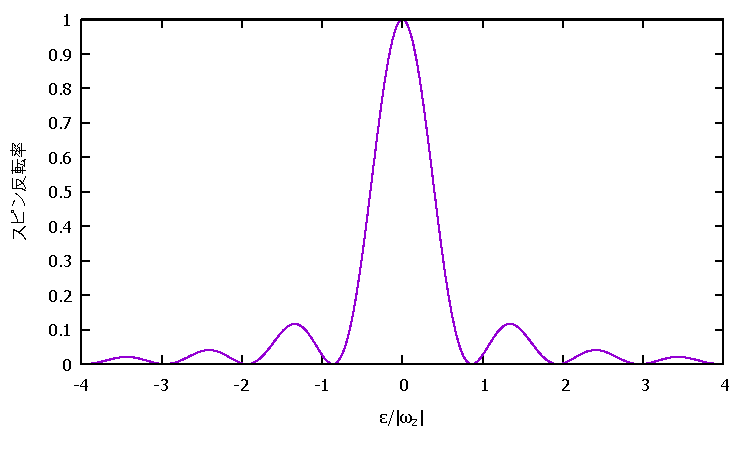
\includegraphics[width=10cm]{nonreso/nonreso_reversalrate.pdf}
\caption{スピン反転率}
\label{Nonreso_fig_reversalrate}
\end{center}
\end{figure}


\subsection{スピン干渉の原理}
ではいよいよ必ずしも共鳴条件を満たさない場合のスピン干渉の原理を見てゆこう。

\paragraph{舞台とあらすじ}
一様磁場中に、理想化されたRFスピンフリッパーふたつとシフタコイルひとつが置かれた状況を考える。系は7つの領域I,II,III,IV,V,VI,VIIからなり、全体に$z$方向一様磁場$B_z$がかけられ、それに加えて領域II,VIに$x$方向振動磁場$2B_r\cos\omega_s t$が、領域IVに$z$方向一様磁場$B$がかけられている。
\begin{figure}[h]
\centering
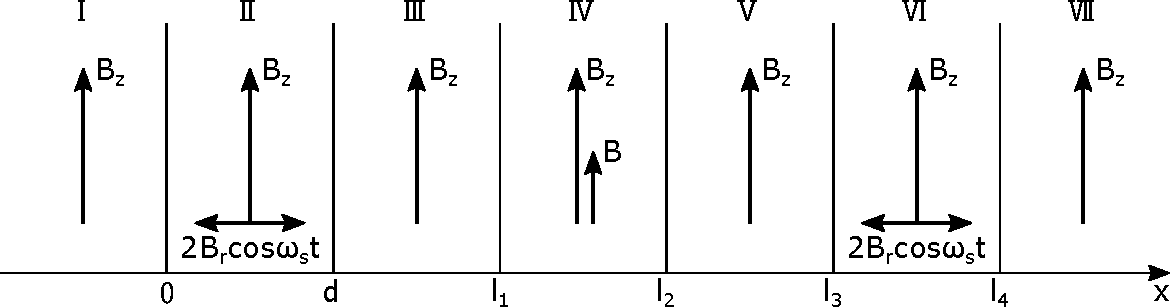
\includegraphics[height=3cm]{nonreso/resonance_setting2.pdf}
\end{figure}

これから述べるように、スピン上向きの中性子が領域Iから入射し、領域I$\sim$VIを通って領域VIIに抜けるとき、領域VIIにおいてスピン上向き中性子を観測する確率は
\begin{equation}
|\psi_\mathrm{VII}^+|^2=N_1(\epsilon)-N_2(\epsilon) \cos (\Omega -\Delta(\epsilon)) -N_3(\epsilon) \sin(\Omega-\Delta(\epsilon)) \label{Nonreso_interference}
\end{equation}
のように書ける。ここで$\Omega$はシフタコイル磁場によって生じた位相差、$\Delta(\epsilon)$は$\epsilon$に依存した定数位相である。

\paragraph{仮定と拝借}
今回は最初から中性子の入射エネルギーはポテンシャルに比べて十分大きいとし、全ての境界で反射は無視する。すると、前節での結果をそのまま拝借することができる。すなわち、領域I,II,IIIにおける波動関数はそれぞれ
\begin{align}
\psi_\mathrm{I}(x,t)&=\begin{pmatrix} 1\\0\end{pmatrix} \e^{i (k_0-\frac{\omega_z}{v})x}\e^{-i\omega_0t}\\
\psi_\mathrm{II}(x,t)&=\begin{pmatrix} \left(\sin^2 \frac{\theta}{2} \e^{i\frac{\omega_A}{v}x} +\cos^2 \frac{\theta}{2} \e^{-i\frac{\omega_A}{v}x} \right) \e^{i(k_0-\frac{\omega_s}{v}) x} \e^{-i\omega_0 t} \\ \sin\frac{\theta}{2}\cos\frac{\theta}{2} \left(\e^{-i\frac{\omega_A}{v}x}-\e^{i\frac{\omega_A}{v}x}\right) \e^{i(k_0-\frac{\omega_s}{v}) x} \e^{-i(\omega_0-\omega_s) t}\end{pmatrix}\\
\psi_\mathrm{III}(x,t)&=\begin{pmatrix} \left(\cos \frac{\omega_A}{v}d +i\frac{\epsilon}{\omega_A} \sin \frac{\omega_A}{v}d\right) \e^{-i\frac{\epsilon}{v} d} \e^{i(k_0-\frac{\omega_z}{v})x}\e^{-i\omega_0t} \\ -i \frac{\omega_r}{\omega_A} \sin \frac{\omega_A}{v}d  \, \e^{i\frac{\epsilon}{v}d} \e^{i(k_0-\frac{\omega_s}{v}+\frac{\omega_z}{v})x}\e^{-i(\omega_0-\omega_s)t} \end{pmatrix}
\end{align}
と書ける。ここで$\epsilon=\omega_s/2-\omega_z,\omega_A=\sqrt{\epsilon^2+\omega_r^2}$であり、$\omega_z=|\mu_n|B_z,\omega_r=|\mu_n|B_r$。$\omega_0$,$v$はそれぞれ中性子の入射エネルギー、速度であり、$k_0=\sqrt{2m\omega_0}$である。その他の記号は前節参照。

\paragraph{領域IV}
領域IVにおけるShr$\ddot{\mathrm{o}}$dinger方程式は
\begin{equation}
i\frac{\del \psi_\mathrm{IV}}{\del t}= \left[-\frac{1}{2m} \frac{\del^2}{\del x^2} +(\omega_z+\omega) \sigma_z\right] \psi_\mathrm{IV}
\end{equation}
ここで$\omega=|\mu_n|B$とした。領域IIIとIVの境界でエネルギーは変化しないので、領域IVにおけるスピン上下成分の波数$k^\pm_\mathrm{IV}$は
\begin{align}
k^+_\mathrm{IV}&=\sqrt{2m(\omega_0-(\omega_z+\omega))}\simeq k_0 -\frac{\omega_z}{v}-\frac{\omega}{v} \\
k^-_\mathrm{IV}&=\sqrt{2m(\omega_0-\omega_s+(\omega_z+\omega))}\simeq k_0 -\frac{\omega_s}{v}+\frac{\omega_z}{v}+\frac{\omega}{v}
\end{align}
となる。反射波を無視し、領域IIIとIVの境界($x=l_1$)で波動関数を接続すると
\begin{equation}
\psi_\mathrm{IV}=\begin{pmatrix} \left(\cos \frac{\omega_A}{v}d +i\frac{\epsilon}{\omega_A} \sin \frac{\omega_A}{v}d\right) \e^{-i\frac{\epsilon}{v} d} \e^{-i\frac{\omega}{v} (x-l_1)} \e^{i(k_0-\frac{\omega_z}{v})x}\e^{-i\omega_0t} \\ -i \frac{\omega_r}{\omega_A} \sin \frac{\omega_A}{v}d  \, \e^{i\frac{\epsilon}{v}d} \e^{i\frac{\omega}{v}(x-l_1)} \e^{i(k_0-\frac{\omega_s}{v}+\frac{\omega_z}{v})x}\e^{-i(\omega_0-\omega_s)t} \end{pmatrix}
\end{equation}
を得る。

\paragraph{領域V}
領域VにおけるShr$\ddot{\mathrm{o}}$dinger方程式は領域I,IIIと等しく、
\begin{equation}
i\frac{\del \psi_\mathrm{V}}{\del t}= \left[-\frac{1}{2m} \frac{\del^2}{\del x^2} +\omega_z \sigma_z\right] \psi_\mathrm{V}
\end{equation}
である。領域VIと同様にして、反射波を無視し、領域IVとVの境界($x=l_2$)で波動関数を接続すると
\begin{equation}
\psi_\mathrm{V}=\begin{pmatrix} \left(\cos \frac{\omega_A}{v}d +i\frac{\epsilon}{\omega_A} \sin \frac{\omega_A}{v}d\right) \e^{-i\frac{\epsilon}{v} d} \e^{-i\frac{\omega}{v} d'} \e^{i(k_0-\frac{\omega_z}{v})x}\e^{-i\omega_0t} \\ -i \frac{\omega_r}{\omega_A} \sin \frac{\omega_A}{v}d  \, \e^{i\frac{\epsilon}{v}d} \e^{i\frac{\omega}{v} d'} \e^{i(k_0-\frac{\omega_s}{v}+\frac{\omega_z}{v})x}\e^{-i(\omega_0-\omega_s)t} \end{pmatrix} \label{Nonreso_psi5}
\end{equation}
を得る。ここで$l_2-l_1=d'$を用いた。

\paragraph{領域VI}
領域VIにおける磁場を、領域IIと同じ$z$方向一様磁場と同位相の$x$方向振動磁場
\begin{equation}
\bm{B}_\mathrm{VI}=\hat{\bm{x}}(2B_r)\cos\omega_s t +\hat{\bm{z}}B_z
\end{equation}
とすると、$B_r \ll B_z$のとき
\begin{equation}
\bm{B}_\mathrm{VI} \simeq \hat{\bm{x}} B_r\cos \omega_s t+\hat{\bm{y}} B_r \sin \omega_s t+\hat{\bm{z}} B_z
\end{equation}
と近似でき、前節と同じ議論により領域VIにおける波動関数は次のように書ける:
\begin{equation}
\psi_\mathrm{VI}=\begin{pmatrix} \left(D^+\cos\frac{\theta}{2} \e^{-i\frac{\omega_A}{v} x}-D^-\sin\frac{\theta}{2} \e^{i\frac{\omega_A}{v}x} \right) \e^{i(k_0-\frac{\omega_s}{2v})x} \e^{-i\omega_0 t} \\ \left(D^+\sin\frac{\theta}{2}\e^{-i\frac{\omega_A}{v} x}+D^-\cos\frac{\theta}{2}\e^{i\frac{\omega_A}{v} x}\right) \e^{i(k_0-\frac{\omega_s}{2v})x} \e^{-i(\omega_0-\omega_s) t} \end{pmatrix}
\end{equation}
ここで入射エネルギーは十分大きいとして反射波を無視し、波数を
\begin{equation}
k^\pm_1 =\sqrt{2m\left(\omega_0-\frac{\omega_s}{2}\mp\omega_A\right)} \simeq k_0 -\frac{\omega_s}{2v} \mp\frac{\omega_A}{v}
\end{equation}
と近似した。また、$\cos \theta = -\epsilon/\omega_A,\sin\theta=\omega_r/\omega_A$であり、$D^\pm$は定数である。

\paragraph{領域VとVIの接続}簡単のため式(\ref{Nonreso_psi5})で
\begin{align}
\alpha^+ &= \left(\cos \frac{\omega_A}{v}d +i\frac{\epsilon}{\omega_A} \sin \frac{\omega_A}{v}d\right) \e^{-i\frac{\epsilon}{v} d} \e^{-i\frac{\omega}{v} d} \label{Nonreso_alpha+}\\
\alpha^-&=-i \frac{\omega_r}{\omega_A} \sin \frac{\omega_A}{v}d  \, \e^{i\frac{\epsilon}{v}d} \e^{i\frac{\omega}{v} d} \label{Nonreso_alpha-}
\end{align}
とおき、領域Vでの波動関数を
\begin{equation}
\psi_\mathrm{V} =\begin{pmatrix} \alpha^+ \e^{i(k_0-\frac{\omega_z}{v})x}\e^{-i\omega_0t}\\ \alpha^- \e^{i(k_0-\frac{\omega_s}{v}+\frac{\omega_z}{v})x}\e^{-i(\omega_0-\omega_s)t} \end{pmatrix}
\end{equation}
とかく。領域VとVIの境界($x=l_3$)における接続を考えて、次の2式を得る:
\begin{align}
&\left\{\begin{array}{l} \left(D^+ \cos\frac{\theta}{2} \e^{-i\frac{\omega_A}{v} l_3}-D^-\sin\frac{\theta}{2} \e^{i\frac{\omega_A}{v}l_3}\right) \e^{i(k_0-\frac{\omega_s}{2v})l_3} =\alpha^+ \e^{i(k_0-\frac{\omega_z}{v})l_3} \\ \left(D^+\sin\frac{\theta}{2}\e^{-i\frac{\omega_A}{v} l_3}+D^-\cos\frac{\theta}{2}\e^{i\frac{\omega_A}{v} l_3}\right) \e^{i(k_0-\frac{\omega_s}{2v})l_3} =\alpha^- \e^{i(k_0-\frac{\omega_s}{v}+\frac{\omega_z}{v})l_3}\end{array} \right. \notag \\
&\Rightarrow \left\{\begin{array}{l} D^+ \cos\frac{\theta}{2} \e^{-i\frac{\omega_A}{v} l_3}-D^-\sin\frac{\theta}{2} \e^{i\frac{\omega_A}{v}l_3} =\alpha^+ \e^{i\frac{\epsilon}{v}l_3} \\ D^+\sin\frac{\theta}{2}\e^{-i\frac{\omega_A}{v} l_3}+D^-\cos\frac{\theta}{2}\e^{i\frac{\omega_A}{v} l_3} =\alpha^- \e^{-i\frac{\epsilon}{v}l_3}\end{array} \right. \notag \\
&\Rightarrow \left\{\begin{array}{l} D^+ =\left(\alpha^+ \cos\frac{\theta}{2}\e^{i\frac{\epsilon}{v}l_3} +\alpha^- \sin\frac{\theta}{2}\e^{-i\frac{\epsilon}{v}l_3}\right) \e^{i\frac{\omega_A}{v} l_3} \\ D^-=\left(-\alpha^+ \sin\frac{\theta}{2} \e^{i\frac{\epsilon}{v}l_3} +\alpha^-\cos\frac{\theta}{2}\e^{-i\frac{\epsilon}{v}l_3} \right)\e^{-i\frac{\omega_A}{v} l_3} \end{array} \right.
\end{align}
したがって
\begin{equation}
\psi_\mathrm{VI} =\left( \begin{array}{l} \left[\alpha^+ \left(\cos^2\frac{\theta}{2}\e^{-i\frac{\omega_A}{v}(x-l_3)} +\sin^2\frac{\theta}{2}\e^{i\frac{\omega_A}{v}(x-l_3)} \right)\e^{i\frac{\epsilon}{v}l_3} \right. \\ \hspace{2cm}\left. +\alpha^- \sin\frac{\theta}{2}\cos\frac{\theta}{2} \left(\e^{-i\frac{\omega_A}{v}(x-l_3)}-\e^{i\frac{\omega_A}{v}(x-l_3)}\right)\e^{-i\frac{\epsilon}{v}l_3}\right]\e^{i(k_0-\frac{\omega_s}{2v})x}\e^{-\omega_0t} \\ \left[\alpha^+ \sin\frac{\theta}{2}\cos\frac{\theta}{2} \left(\e^{-i\frac{\omega_A}{v}(x-l_3)}-\e^{i\frac{\omega_A}{v}(x-l_3)}\right)\e^{i\frac{\epsilon}{v}l_3} \right. \\ \hspace{2cm} \left. +\alpha^- \left(\sin^2\frac{\theta}{2}\e^{-i\frac{\omega_A}{v}(x-l_3)} +\cos^2\frac{\theta}{2}\e^{i\frac{\omega_A}{v}(x-l_3)} \right) \e^{-i\frac{\epsilon}{v}l_3}\right] \e^{i(k_0-\frac{\omega_s}{2v})x} \e^{-i(\omega_0-\omega_s) t} \end{array}\right)
\end{equation}
となる。

\paragraph{領域VII}
領域VにおけるShr$\ddot{\mathrm{o}}$dinger方程式は領域I,III,Vと同じく
\begin{equation}
i\frac{\del \psi_\mathrm{VII}}{\del t}= \left[-\frac{1}{2m} \frac{\del^2}{\del x^2} +\omega_z \sigma_z\right] \psi_\mathrm{VII}
\end{equation}
であり、領域VIとVIIの境界($x=l_4$)で波動関数を接続すると次式を得る:
\begin{align}
\psi_\mathrm{VII} &=\left( \begin{array}{l} \left[\alpha^+ \left(\cos^2\frac{\theta}{2}\e^{-i\frac{\omega_A}{v}(l_4-l_3)} +\sin^2\frac{\theta}{2}\e^{i\frac{\omega_A}{v}(l_4-l_3)} \right)\e^{i\frac{\epsilon}{v}l_3} \right. \\ \hspace{1cm}\left. +\alpha^- \sin\frac{\theta}{2}\cos\frac{\theta}{2} \left(\e^{-i\frac{\omega_A}{v}(l_4-l_3)}-\e^{i\frac{\omega_A}{v}(l_4-l_3)}\right)\e^{-i\frac{\epsilon}{v}l_3}\right]\e^{i(k_0-\frac{\omega_s}{2v})l_4} \e^{i(k_0-\frac{\omega_z}{v})(x-l_4)} \e^{-\omega_0t} \\ \left[\alpha^+ \sin\frac{\theta}{2}\cos\frac{\theta}{2} \left(\e^{-i\frac{\omega_A}{v}(l_4-l_3)}-\e^{i\frac{\omega_A}{v}(l_4-l_3)}\right)\e^{i\frac{\epsilon}{v}l_3} \right. \\ \hspace{1cm} \left. +\alpha^- \left(\sin^2\frac{\theta}{2}\e^{-i\frac{\omega_A}{v}(l_4-l_3)} +\cos^2\frac{\theta}{2}\e^{i\frac{\omega_A}{v}(l_4-l_3)} \right) \e^{-i\frac{\epsilon}{v}l_3}\right] \e^{i(k_0-\frac{\omega_s}{2v})l_4} \e^{i(k_0-\frac{\omega_s}{v}+\frac{\omega_z}{v})(x-l_4)} \e^{-i(\omega_0-\omega_s) t} \end{array}\right) \notag \\
&=\left( \begin{array}{l} \left[\alpha^+ \left(\cos^2\frac{\theta}{2}\e^{-i\frac{\omega_A}{v}d} +\sin^2\frac{\theta}{2}\e^{i\frac{\omega_A}{v}d} \right)\e^{i\frac{\epsilon}{v}l_3} \right. \\ \hspace{2cm}\left. +\alpha^- \sin\frac{\theta}{2}\cos\frac{\theta}{2} \left(\e^{-i\frac{\omega_A}{v}d}-\e^{i\frac{\omega_A}{v}d}\right)\e^{-i\frac{\epsilon}{v}l_3}\right]\e^{-i\frac{\epsilon}{v}l_4}\e^{i(k_0-\frac{\omega_z}{v})x} \e^{-\omega_0t} \\ \left[\alpha^+ \sin\frac{\theta}{2}\cos\frac{\theta}{2} \left(\e^{-i\frac{\omega_A}{v}d}-\e^{i\frac{\omega_A}{v}d}\right)\e^{i\frac{\epsilon}{v}l_3} \right. \\ \hspace{2cm} \left. +\alpha^- \left(\sin^2\frac{\theta}{2}\e^{-i\frac{\omega_A}{v}d} +\cos^2\frac{\theta}{2}\e^{i\frac{\omega_A}{v}d} \right) \e^{-i\frac{\epsilon}{v}l_3}\right] \e^{i\frac{\epsilon}{v}l_4} \e^{i(k_0-\frac{\omega_s}{v}+\frac{\omega_z}{v})x} \e^{-i(\omega_0-\omega_s) t} \end{array}\right)
\end{align}
ここで$l_4-l_3=d$を用いた。さらに$\cos\theta=-\epsilon/\omega_A,\sin\theta=\omega_r/\omega_A$より
\begin{align}
&\cos^2 \frac{\theta}{2} \e^{-i\frac{\omega_A}{v}d} +\sin^2 \frac{\theta}{2} \e^{i\frac{\omega_A}{v}d} =\cos \frac{\omega_A}{v}d +i\frac{\epsilon}{\omega_A} \sin \frac{\omega_A}{v}d \\
&\sin^2 \frac{\theta}{2} \e^{-i\frac{\omega_A}{v}d} +\cos^2 \frac{\theta}{2} \e^{i\frac{\omega_A}{v}d} =\left(\cos^2 \frac{\theta}{2} \e^{-i\frac{\omega_A}{v}d} +\sin^2 \frac{\theta}{2} \e^{i\frac{\omega_A}{v}d}\right)^\dagger=\cos \frac{\omega_A}{v}d -i\frac{\epsilon}{\omega_A} \sin \frac{\omega_A}{v}d \\
&\sin\frac{\theta}{2}\cos\frac{\theta}{2} \left(\e^{-i\frac{\omega_A}{v}d}-\e^{i\frac{\omega_A}{v}d}\right) = -i \frac{\omega_r}{\omega_A} \sin \frac{\omega_A}{v}d
\end{align}
を用い、(\ref{Nonreso_alpha+}),(\ref{Nonreso_alpha-})の$\alpha^\pm$を代入して
\begin{align}
\psi_\mathrm{VII} &= \left( \begin{array}{l} \left[\left(\cos \frac{\omega_A}{v}d +i\frac{\epsilon}{\omega_A} \sin \frac{\omega_A}{v}d\right)^2\e^{i\frac{\epsilon}{v}(l_3-d)}\e^{-i\frac{\omega}{v}d'} \right. \\ \hspace{2cm}\left. +\left(-i \frac{\omega_r}{\omega_A} \sin \frac{\omega_A}{v}d\right)^2\e^{-i\frac{\epsilon}{v}(l_3-d)}\e^{i\frac{\omega}{v}d'} \right]\e^{-i\frac{\epsilon}{v}l_4}\e^{i(k_0-\frac{\omega_z}{v})x} \e^{-\omega_0t} \\ \left[\left(\cos \frac{\omega_A}{v}d +i\frac{\epsilon}{\omega_A} \sin \frac{\omega_A}{v}d\right) \left(-i \frac{\omega_r}{\omega_A} \sin \frac{\omega_A}{v}d\right) \e^{i\frac{\epsilon}{v}(l_3-d)}\e^{-i\frac{\omega}{v}d'} \right. \\ \hspace{1cm} \left. +\left(-i \frac{\omega_r}{\omega_A} \sin \frac{\omega_A}{v}d\right) \left(\cos \frac{\omega_A}{v}d -i\frac{\epsilon}{\omega_A} \sin \frac{\omega_A}{v}d\right) \e^{-i\frac{\epsilon}{v}(l_3-d)}\e^{i\frac{\omega}{v}d'} \right] \e^{i\frac{\epsilon}{v}l_4} \e^{i(k_0-\frac{\omega_s}{v}+\frac{\omega_z}{v})x} \e^{-i(\omega_0-\omega_s) t} \end{array}\right) \notag \\
&=\left( \begin{array}{l} \left[\left(\cos \frac{\omega_A}{v}d +i\frac{\epsilon}{\omega_A} \sin \frac{\omega_A}{v}d\right)^2\e^{i\frac{\epsilon}{v}L'}\e^{-i\frac{\omega}{v}d'} \right. \\ \hspace{2cm}\left. +\left(-i \frac{\omega_r}{\omega_A} \sin \frac{\omega_A}{v}d\right)^2\e^{-i\frac{\epsilon}{v}L'}\e^{i\frac{\omega}{v}d'} \right]\e^{-i\frac{\epsilon}{v}L}\e^{i(k_0-\frac{\omega_z}{v})x} \e^{-\omega_0t} \\ \left(-i \frac{\omega_r}{\omega_A} \sin \frac{\omega_A}{v}d\right) \left[\left(\cos \frac{\omega_A}{v}d +i\frac{\epsilon}{\omega_A} \sin \frac{\omega_A}{v}d\right) \e^{i\frac{\epsilon}{v}L'}\e^{-i\frac{\omega}{v}d'} \right. \\ \hspace{2cm} \left. +\left(\cos \frac{\omega_A}{v}d -i\frac{\epsilon}{\omega_A} \sin \frac{\omega_A}{v}d\right) \e^{-i\frac{\epsilon}{v}L'}\e^{i\frac{\omega}{v}d'} \right] \e^{i\frac{\epsilon}{v}L} \e^{i(k_0-\frac{\omega_s}{v}+\frac{\omega_z}{v})x} \e^{-i(\omega_0-\omega_s) t} \end{array}\right)
\end{align}
となる。ここで$l_3-d=L',l_4=L$とした。
%\end{comment}


\paragraph{結末}
以上のようにして、領域Iで
\begin{equation}
\psi_\mathrm{I}(x,t)=\begin{pmatrix} 1\\0\end{pmatrix} \e^{i (k_0-\frac{\omega_z}{v})x}\e^{-i\omega_0t}
\end{equation}
と表された入射中性子は領域II$\sim$VIを通って領域VIIで
\begin{equation}
\psi_\mathrm{VII}(x,t) =\left( \begin{array}{l} \left[\left(\cos \frac{\omega_A}{v}d +i\frac{\epsilon}{\omega_A} \sin \frac{\omega_A}{v}d\right)^2\e^{i\frac{\epsilon}{v}L'}\e^{-i\frac{\omega}{v}d'} \right. \\ \hspace{2cm}\left. +\left(-i \frac{\omega_r}{\omega_A} \sin \frac{\omega_A}{v}d\right)^2\e^{-i\frac{\epsilon}{v}L'}\e^{i\frac{\omega}{v}d'} \right]\e^{-i\frac{\epsilon}{v}L}\e^{i(k_0-\frac{\omega_z}{v})x} \e^{-\omega_0t} \\ \left(-i \frac{\omega_r}{\omega_A} \sin \frac{\omega_A}{v}d\right) \left[\left(\cos \frac{\omega_A}{v}d +i\frac{\epsilon}{\omega_A} \sin \frac{\omega_A}{v}d\right) \e^{i\frac{\epsilon}{v}L'}\e^{-i\frac{\omega}{v}d'} \right. \\ \hspace{2cm} \left. +\left(\cos \frac{\omega_A}{v}d -i\frac{\epsilon}{\omega_A} \sin \frac{\omega_A}{v}d\right) \e^{-i\frac{\epsilon}{v}L'}\e^{i\frac{\omega}{v}d'} \right] \e^{i\frac{\epsilon}{v}L} \e^{i(k_0-\frac{\omega_s}{v}+\frac{\omega_z}{v})x} \e^{-i(\omega_0-\omega_s) t} \end{array}\right)
\end{equation}
という状態をとることがわかった。したがって、領域VIIでスピン上向き中性子を観測する確率は
\begin{align}
|\psi_\mathrm{VII}^+|^2&=\Biggl| \left(\cos \frac{\omega_A}{v}d +i\frac{\epsilon}{\omega_A} \sin \frac{\omega_A}{v}d\right)^2\e^{i\frac{\epsilon}{v}L'}\e^{-i\frac{\omega}{v}d'} +\left(-i \frac{\omega_r}{\omega_A} \sin \frac{\omega_A}{v}d\right)^2\e^{-i\frac{\epsilon}{v}L'}\e^{i\frac{\omega}{v}d'} \Biggr|^2 \notag \\
&=\left[\left(\cos \frac{\omega_A}{v}d +i\frac{\epsilon}{\omega_A} \sin \frac{\omega_A}{v}d\right)^2\e^{i\frac{\epsilon}{v}L'}\e^{-i\frac{\omega}{v}d'} +\left(-i \frac{\omega_r}{\omega_A} \sin \frac{\omega_A}{v}d\right)^2\e^{-i\frac{\epsilon}{v}L'}\e^{i\frac{\omega}{v}d'}\right] \notag\\
&\hspace{2cm} \times \left[\left(\cos \frac{\omega_A}{v}d -i\frac{\epsilon}{\omega_A} \sin \frac{\omega_A}{v}d\right)^2\e^{-i\frac{\epsilon}{v}L'}\e^{i\frac{\omega}{v}d'} +\left(i \frac{\omega_r}{\omega_A} \sin \frac{\omega_A}{v}d\right)^2\e^{i\frac{\epsilon}{v}L'}\e^{-i\frac{\omega}{v}d'}\right] \notag \\
&=\left(\cos^2 \frac{\omega_A}{v}d +\left(\frac{\epsilon}{\omega_A}\right)^2 \sin^2 \frac{\omega_A}{v}d\right)^2+\left(\frac{\omega_r}{\omega_A}\right)^4 \sin^4 \frac{\omega_A}{v}d \notag \\
&\hspace{1cm}  -2\left(\frac{\omega_r}{\omega_A}\right)^2\sin^2\frac{\omega_A}{v}d \left[\left(\cos^2 \frac{\omega_A}{v}d -\left(\frac{\epsilon}{\omega_A}\right)^2 \sin^2 \frac{\omega_A}{v}d\right) \cos \left(\frac{2}{v}(\omega d'-\epsilon L')\right) \right. \notag \\
&\hspace{6.3cm} \left.+2 \frac{\epsilon}{\omega_A} \sin \frac{\omega_A}{v}d \cos \frac{\omega_A}{v}d \sin \left(\frac{2}{v}(\omega d'-\epsilon L')\right)\right]
\end{align}
となる。
\begin{align}
&N_1 = \left(\cos^2 \frac{\omega_A}{v}d +\left(\frac{\epsilon}{\omega_A}\right)^2 \sin^2 \frac{\omega_A}{v}d\right)^2+\left(\frac{\omega_r}{\omega_A}\right)^4 \sin^4 \frac{\omega_A}{v}d \\
&N_2 = 2\left(\frac{\omega_r}{\omega_A}\right)^2\sin^2\frac{\omega_A}{v}d \left(\cos^2 \frac{\omega_A}{v}d -\left(\frac{\epsilon}{\omega_A}\right)^2 \sin^2 \frac{\omega_A}{v}d\right) \\
&N_3 = 4\frac{\epsilon}{\omega_A} \left(\frac{\omega_r}{\omega_A}\right)^2\sin^3\frac{\omega_A}{v}d \cos \frac{\omega_A}{v}d
\end{align}
とおけばこれを
\begin{equation}
|\psi_\mathrm{VII}^+|^2 =N_1 -N_2 \cos \left(\frac{2}{v}(\omega d'-\epsilon L')\right)-N_3 \sin  \left(\frac{2}{v}(\omega d'-\epsilon L')\right) \label{Nonreso_interference2}
\end{equation}
と書くことができる。

いま$\omega_rd/v=\pi/4$,$\epsilon/|\omega_z|=0,0.3,0.5,1.0$のときに$\omega d'/v$と$|\psi_\mathrm{VII}|^2$の関係を図示すると図\ref{Nonreso_fig_interference}のようになる。ただし$L'/d=10$とした。このように理論が予想するところによると、シフタコイルの磁場を変えながら領域VIIでスピン上向き中性子の数を計測すると波打つ干渉のパターンが見られるが、その振幅や位相、振動中心の位置は共鳴からのずれによって異なる。

\begin{figure}[h]
\centering
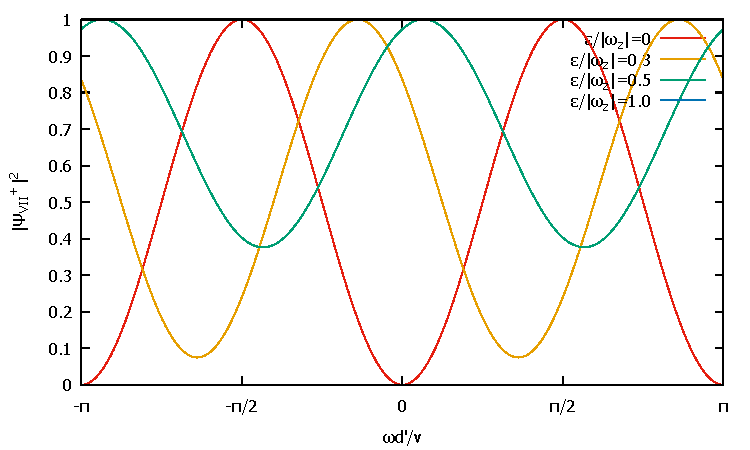
\includegraphics[width=10cm]{nonreso/nonreso_interference.pdf}
\caption{干渉パターン {\footnotesize ($\epsilon/|\omega_z|=1.0$は上に張り付いている)}}
\label{Nonreso_fig_interference}
\vspace{-1cm}
\end{figure}



\renewcommand{\arraystretch}{1}



\section{加速器の原理}
本実験は京都大学小型中性子源KUANS(Kyoto University Accelerator-driven Neutron Source)で行った。本節ではKUANSについて説明する。
KUANSの性能は以下のようになっている。


\begin{table}[htb]
\centering
\begin{tabular}{lcrr}
加速器&陽子線形加速器\\
加速粒子&陽子\\
最大加速エネルギー&3.5MeV\\
最大電流&100 $\mu$ \\
中性子発生ターゲット&Be\\
発生中性子エネルギー&keV~熱中性子(約2000m/s)\\
中性子減速材&ポリエチレン($10\times10\times10$ cm$^3$)\\
\end{tabular}
\end{table}

\begin{figure}[h]
\begin{center}
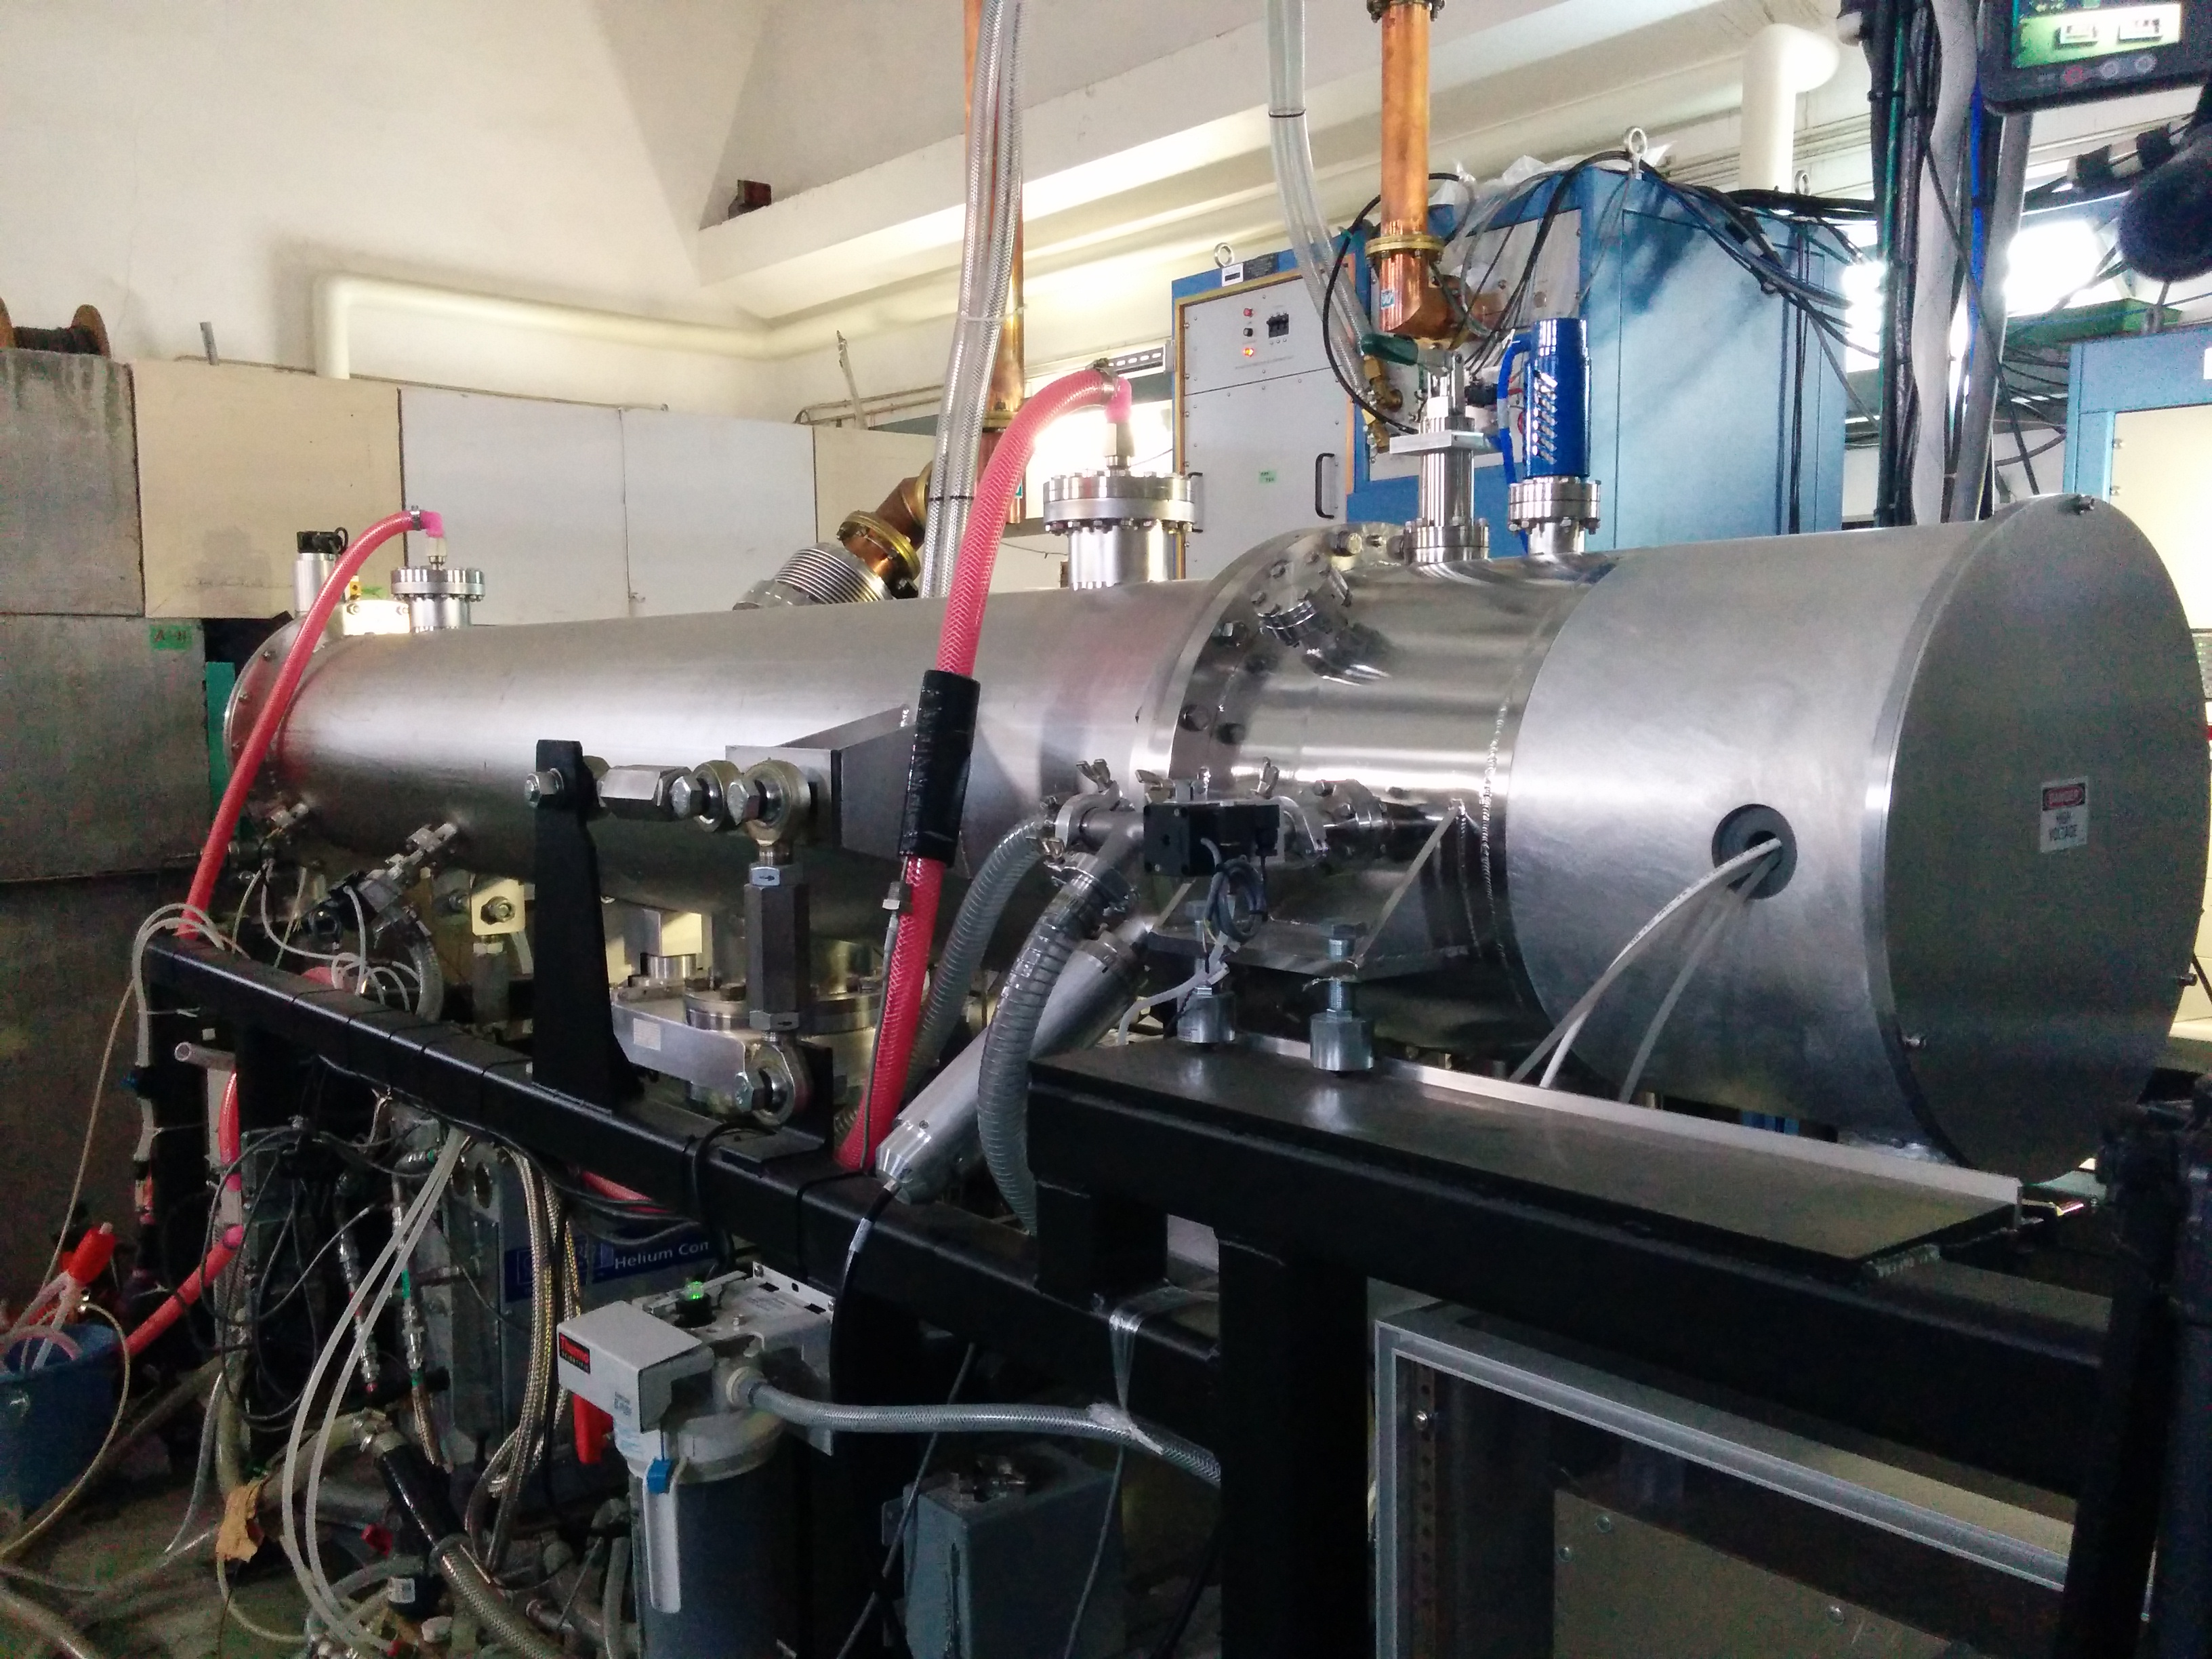
\includegraphics[width=9cm,height=6cm]{accelerator/accphoto.jpg}
\caption{陽子線形加速器}
\end{center}
\end{figure}

\subsection{中性子発生方法}
まず陽子線形加速器によって陽極で発生させた陽子を電圧で加速させ、シールド内に収められているBeターゲットへと衝突させる。\\
この際起こる以下の反応、\begin{equation}
\ce{p + {^{9}Be} ->n + {^{9}B}}\end{equation}
によって中性子を発生させている。
しかしこのままの中性子は速すぎて実験に向かないので、KUANSでは減速材を用いて減速させ熱中性子とした後に、陽子ビームの向きと90$^{\circ}$をなす方向に導いて実験用中性子ビームとして利用している。
\subsection {TOF(Time Of Flight)}
TOFとは一般的に粒子が加速されてから検出器に入るまでに要する時間のことである。
以降、本実験におけるTOFとは陽子線形加速器に電圧が印加されてから、発生した中性子が検出器に入るまでに要する時間のことを指すこととする。
このTOFは以下のように表せる。
\begin{equation}TOF=T_a+T_m+T_f\end{equation}
$T_a:陽子が加速されてからBeターゲットに当たるまでに要する時間$\\
$T_m:発生した中性子が減速材中で熱平衡に達するまでに要する時間$\\
$T_f:減速材をでた中性子が検出器に入るまでに要する時間の飛行時間$\\
本加速器においては、$T_a$は無視できる程小さく、また$T_m$は平均で約70$\mu$sである。
実際に測定されたTOFから$T_m$の平均値70$\mu$sを引いたものを補正したTOFと呼び、tとする。
本実験では波長が重要な値となるのでtから以下の式によって中性子の波長を算出した。
\begin{equation}
{\lambda}={\frac{ht}{md}}
\end{equation}
$d:減速材から検出器までの距離$\\
本実験においては約1100m/s、波長にして約3.5$\AA$の範囲にある中性子を用いた。
\subsection {中性子のTOF分布}
\begin{figure}[h]
\centering
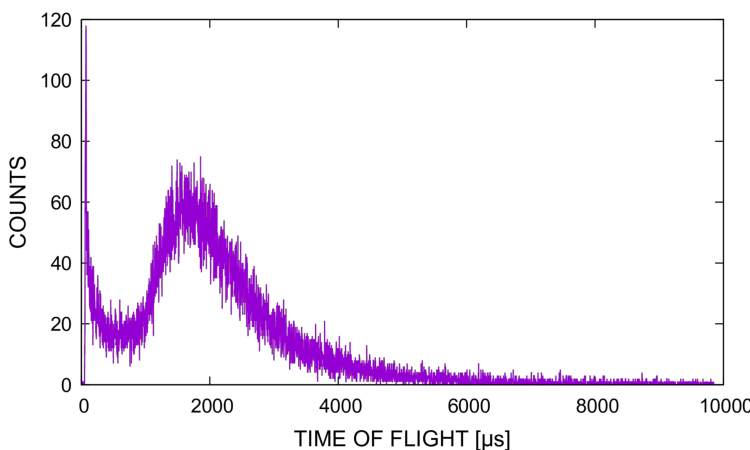
\includegraphics[width=9cm]{accelerator/TOF.pdf}
\caption{実際に測定したTOF分布}
\end{figure}
領域①は減速材で熱平衡に達しなかった高速中性子に因る寄与であり、領域②は熱平衡に達した熱中性子に因る寄与である。
後者TOF分布$F(t)$は\begin{equation}F(t)\propto \frac{1}{t^{3}}\exp(-\frac{md^2}{2kTt^2}) \end{equation}で与えられる。
\subsubsection{補足:中性子のフラックス}
検出器に速度$v$で入射する中性子の数を考える。
検出器の表面の微小面積要素$dS$に時間$dt$の間に速度$v=(v_x,v_y,v_z)$で入射する中性子数$dN$は$n$を中性子数密度として
\begin{equation}
dN=nv_xdtf(v_x,v_y,v_z)dS
\end{equation}
で与えられる。\\
但し、$f(v_x,v_y,v_z)$は熱平衡にあり当方的な速度分布を持つ粒子が従う確率密度関数で以下の式で与えられる。
\begin{equation}
f(v_x,v_y,v_z)={(\frac{m}{2\pi kT})}^{\frac{3}{2}}\exp\{-\frac{m}{2kT}(v^2_x+v^2_y+v^2_z)\} 
\end{equation}
後のため$f(v_x,v_y,v_z)$を極座標に変換すると、
\begin{equation}
f(v_x,v_y,v_z) \rightarrow f(v,\theta,\phi)={(\frac{m}{2\pi kT})}^{\frac{3}{2}}v^2\exp(-\frac{mv^2}{2kT})
\end{equation}
この微小面積要素$dS$に入射する粒子には様々な角度を持つものがあるので、$dS$に入射可能な角度範囲について積分すると、
\begin{eqnarray*}
 \iint dN\sin\theta d\theta d\phi &=&\iint nvdtf(v_x,v_y,v_z)\cos\theta \sin\theta d\theta d\phi dS \\ 
&=&ndtdS \hspace{-2pt}\iint \hspace{-2pt}{(\frac{m}{2\pi kT})}^{\frac{3}{2}}v^3\exp(-\frac{mv^2}{2kT})\cos\theta \sin\theta d\theta d\phi  \\
&=&ndtdS{(\frac{m}{2\pi kT})}^{\frac{3}{2}} v^3\exp(-\frac{mv^2}{2kT}) \hspace{-2pt}\int \hspace{-2pt}\cos\theta\sin\theta d\theta \hspace{-2pt}\int \hspace{-2pt} d\phi \\
&=&Cv^3\exp(-\frac{mv^2}{2kT})dtdS
\end{eqnarray*}
ここでCは速度には依らないが、検出器表面の場所には依存する関数である。
これより検出器に単位時間あたりに入射する全粒子数$N$は,
\begin{eqnarray*}
N &=&
\int\limits_{\text{} 検出器表面}Cv^3\exp(-\frac{mv^2}{2kT})dS \\
&\propto& v^3\exp(-\frac{mv^2}{2kT})
\end{eqnarray*}
この$v$を$t=\frac{d}{v}$で書き換えたものが先に示したTOF分布$F(t)$である。
\newpage
\subsection{Lim}
LiM(Lithium Monitor)はシールド内の減速材の後に置かれていて、ビームの一部を削り中性子ビーム強度を計測する役割を持つ。
このLiMの値と取り出した中性子ビーム強度は比例すると考えて本実験で規格化する際に用いた。
LiMの値を実際に測定するとグラフのようになった。但し、横軸は時刻である。
\begin{figure}[h]
\centering
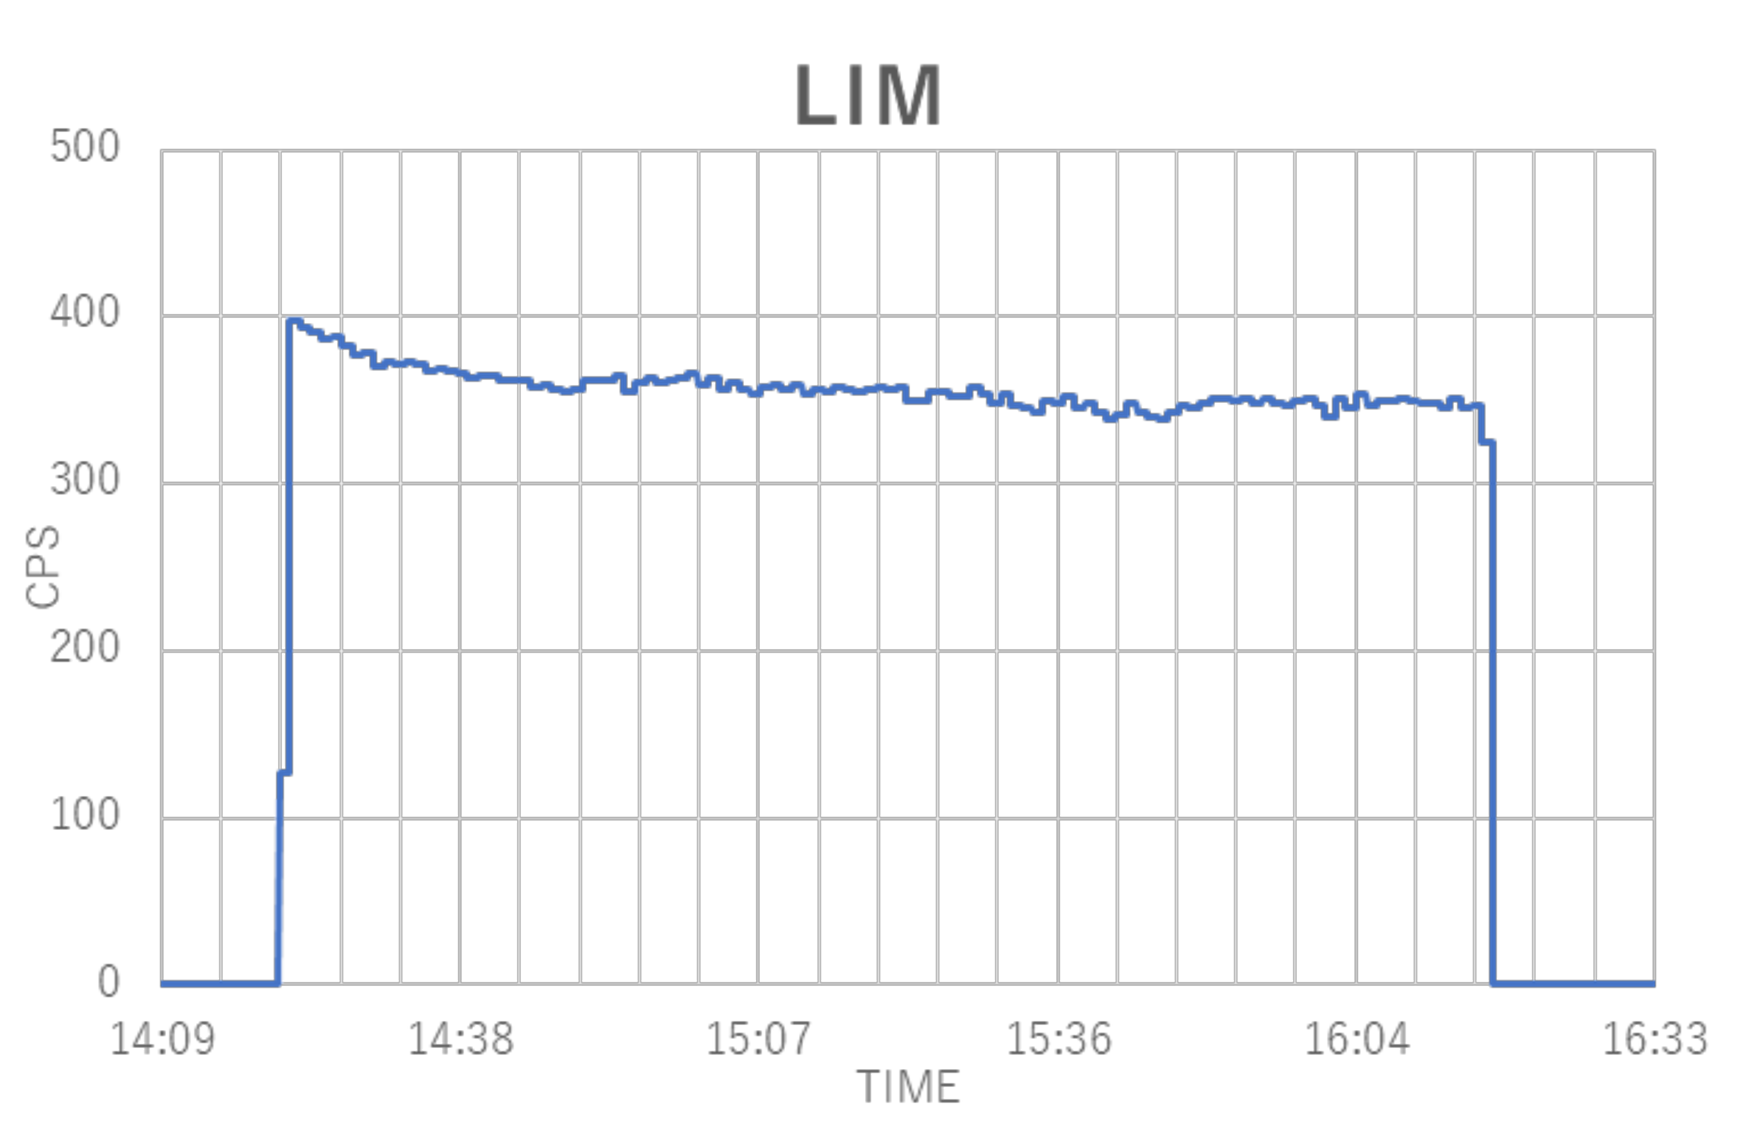
\includegraphics[width=9cm,height=8cm]{accelerator/LiM.pdf}\caption{LiMの時間変化}
\end{figure}\\
グラフを見ると分かるように本加速器は一定強度ではなく次第にビーム強度が低下し、ある値の周辺で変動する特徴があることが分かる。




\section{実験装置}
本節では実験において使用した装置を説明する。
\subsection{ガイド磁場コイル}
ガイド磁場コイルには二つの役割を持っている\\
1.実験装置全体に渡って中性子の量子化軸を定める\\
2.垂直方向に地磁気を無視できる程の大きさの磁場を一様に印加する\\
特に二つ目の役割は重要であり磁場の大きさが地磁気に比べて十分大きくないと地磁気によるスピンの反転が起きてしまうことになる。\\
また、磁場の一様性は中性子が通過する場所によって干渉条件が大きくずれないことを保証する。\\
実験ではガイド磁場コイルに5.5Aの電流を流し、ビーム軸上で磁場の強さは約12~13Gとなった。\\
なお電流を5.5A流すとガイド磁場コイルの温度が60$^\circ$C以上になる部分もあったため、3台の扇風機で空冷しながら実験を行った。
\begin{figure}[h]
\begin{center}
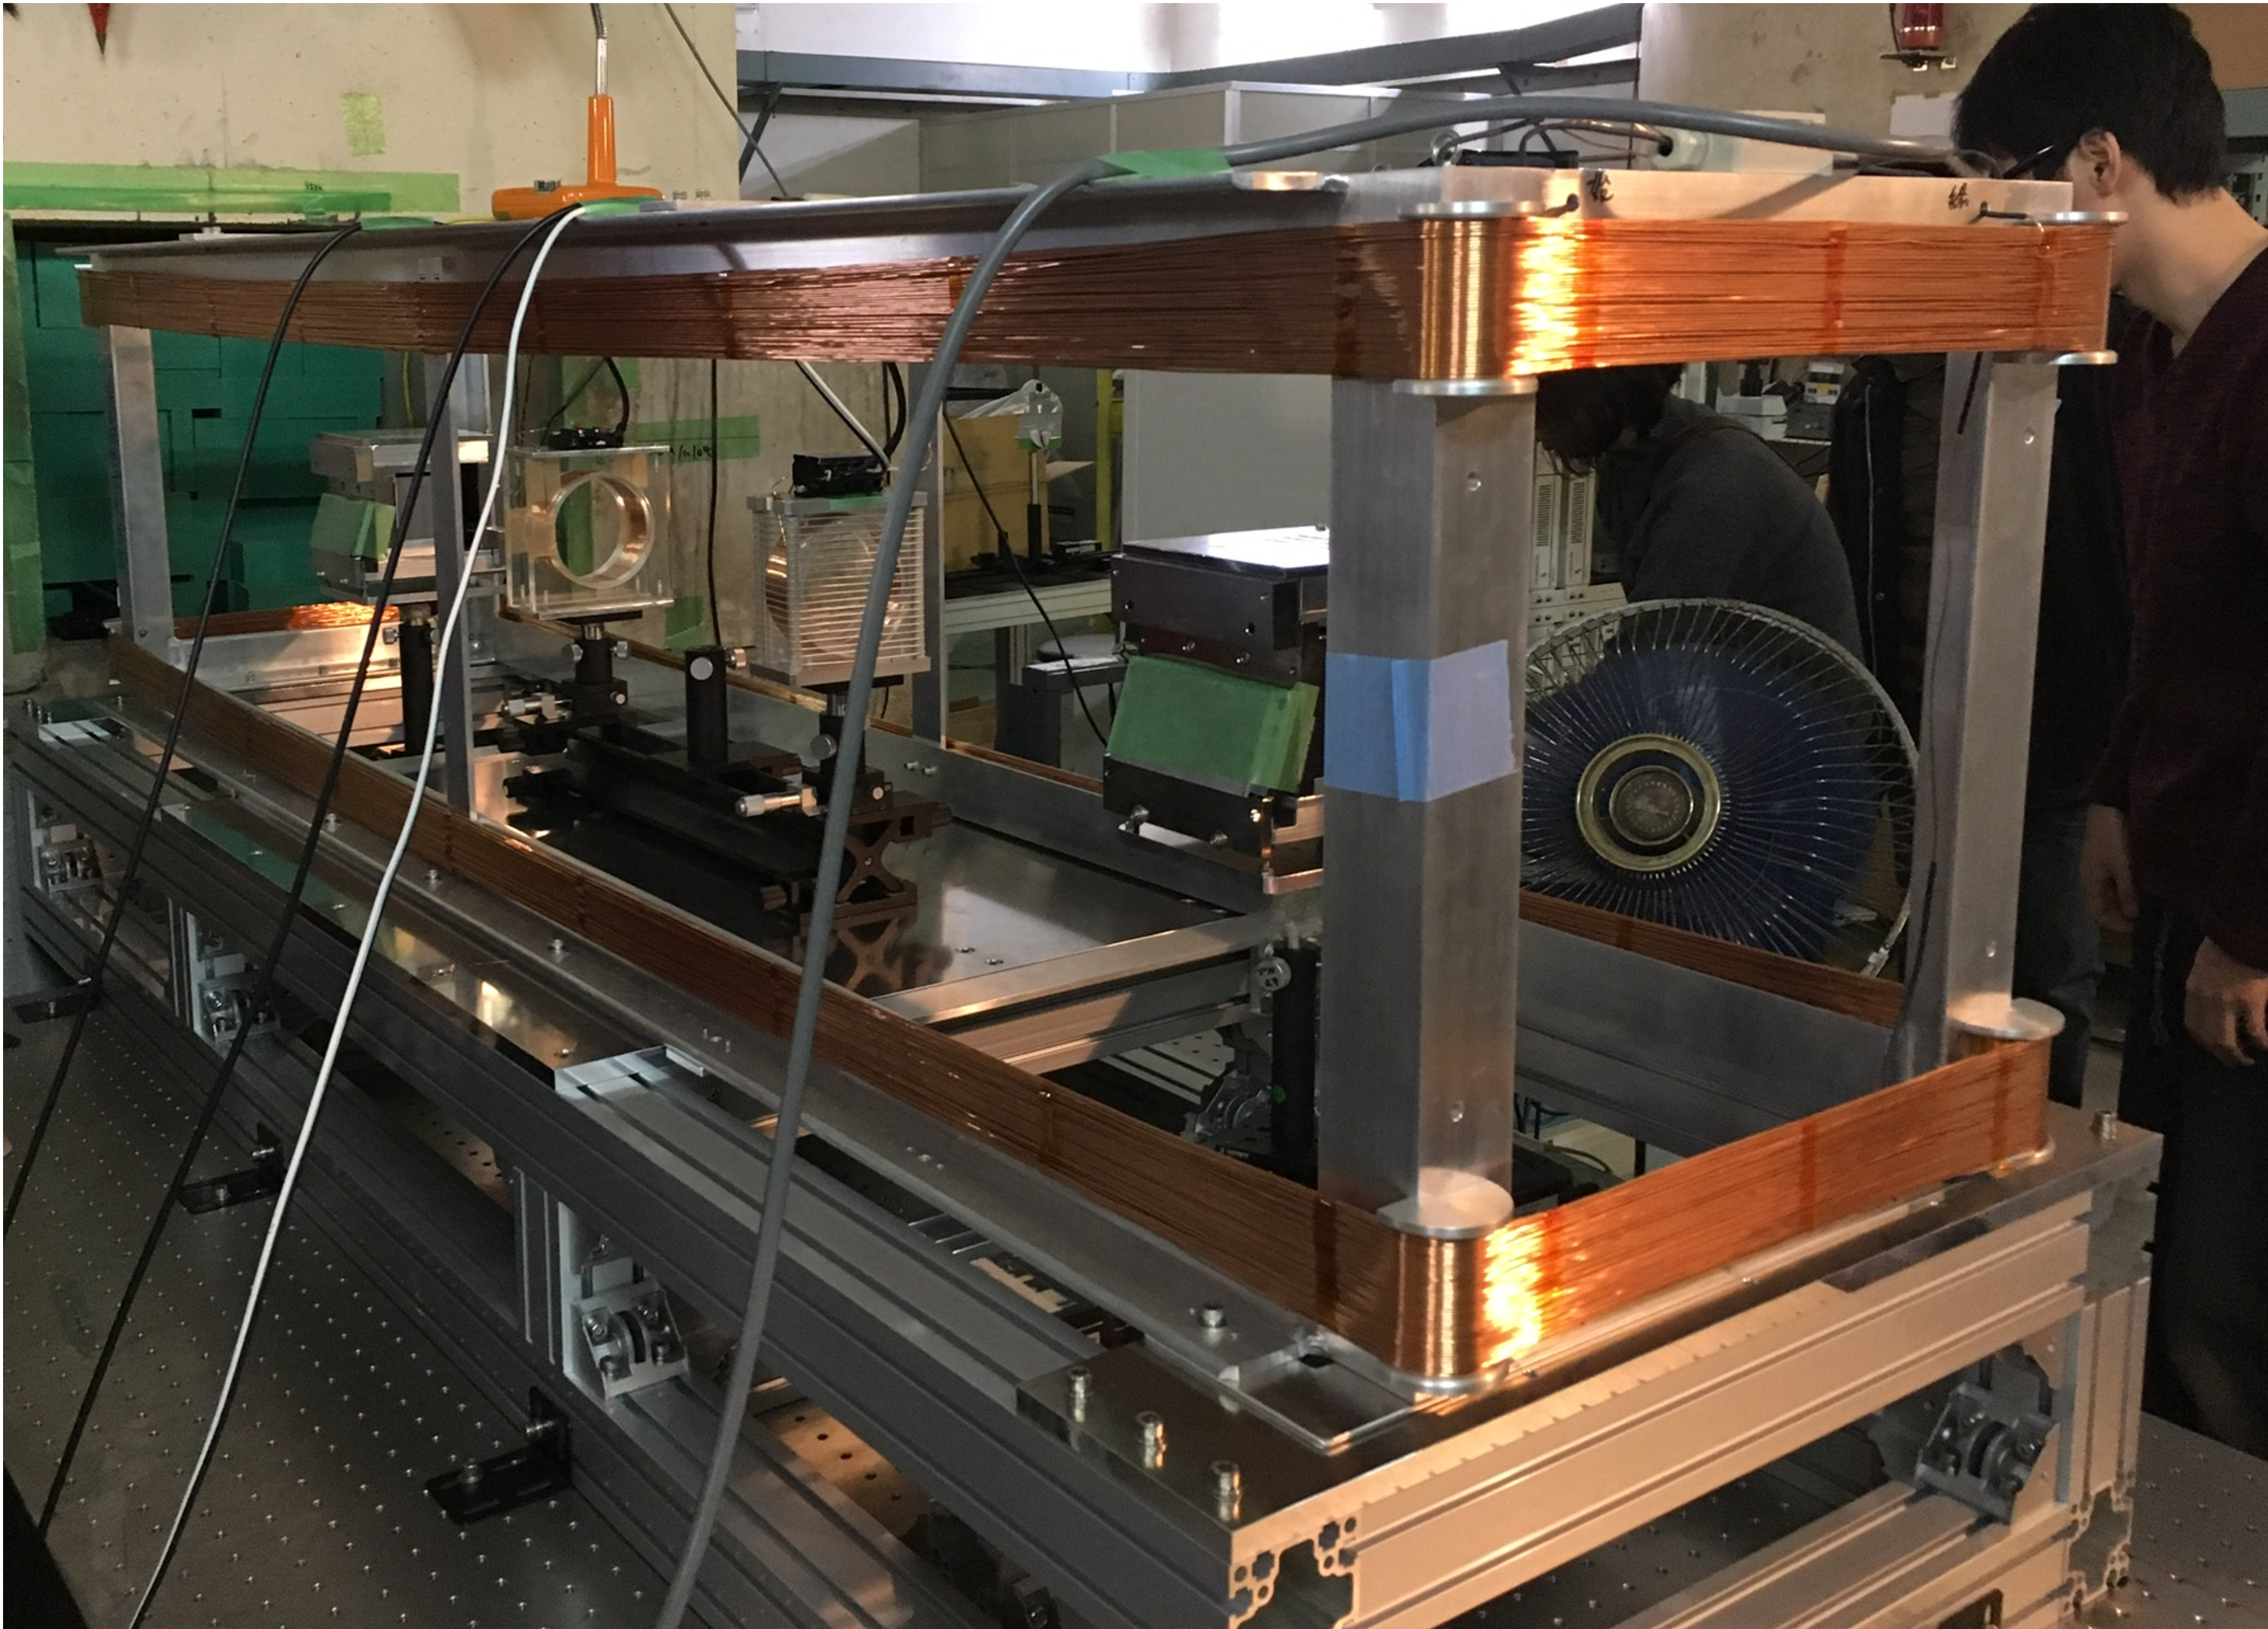
\includegraphics[width=8cm,height=5cm]{device/coilphoto.pdf}\caption{ガイド磁場コイル}
\end{center}
\end{figure}
\subsection{スピンフリッパ―}
スピンフリッパ―は入射中性子をスピン上向きと下向きの状態の重ね合わせにする役割を持つ。\\
装置としての構造は極めて単純で普通のソレノイドコイルである。コイルに高周波電流を流すことによって高周波磁場を作り出しスピンをフリップさせている。
\begin{figure}[H]
\begin{center}
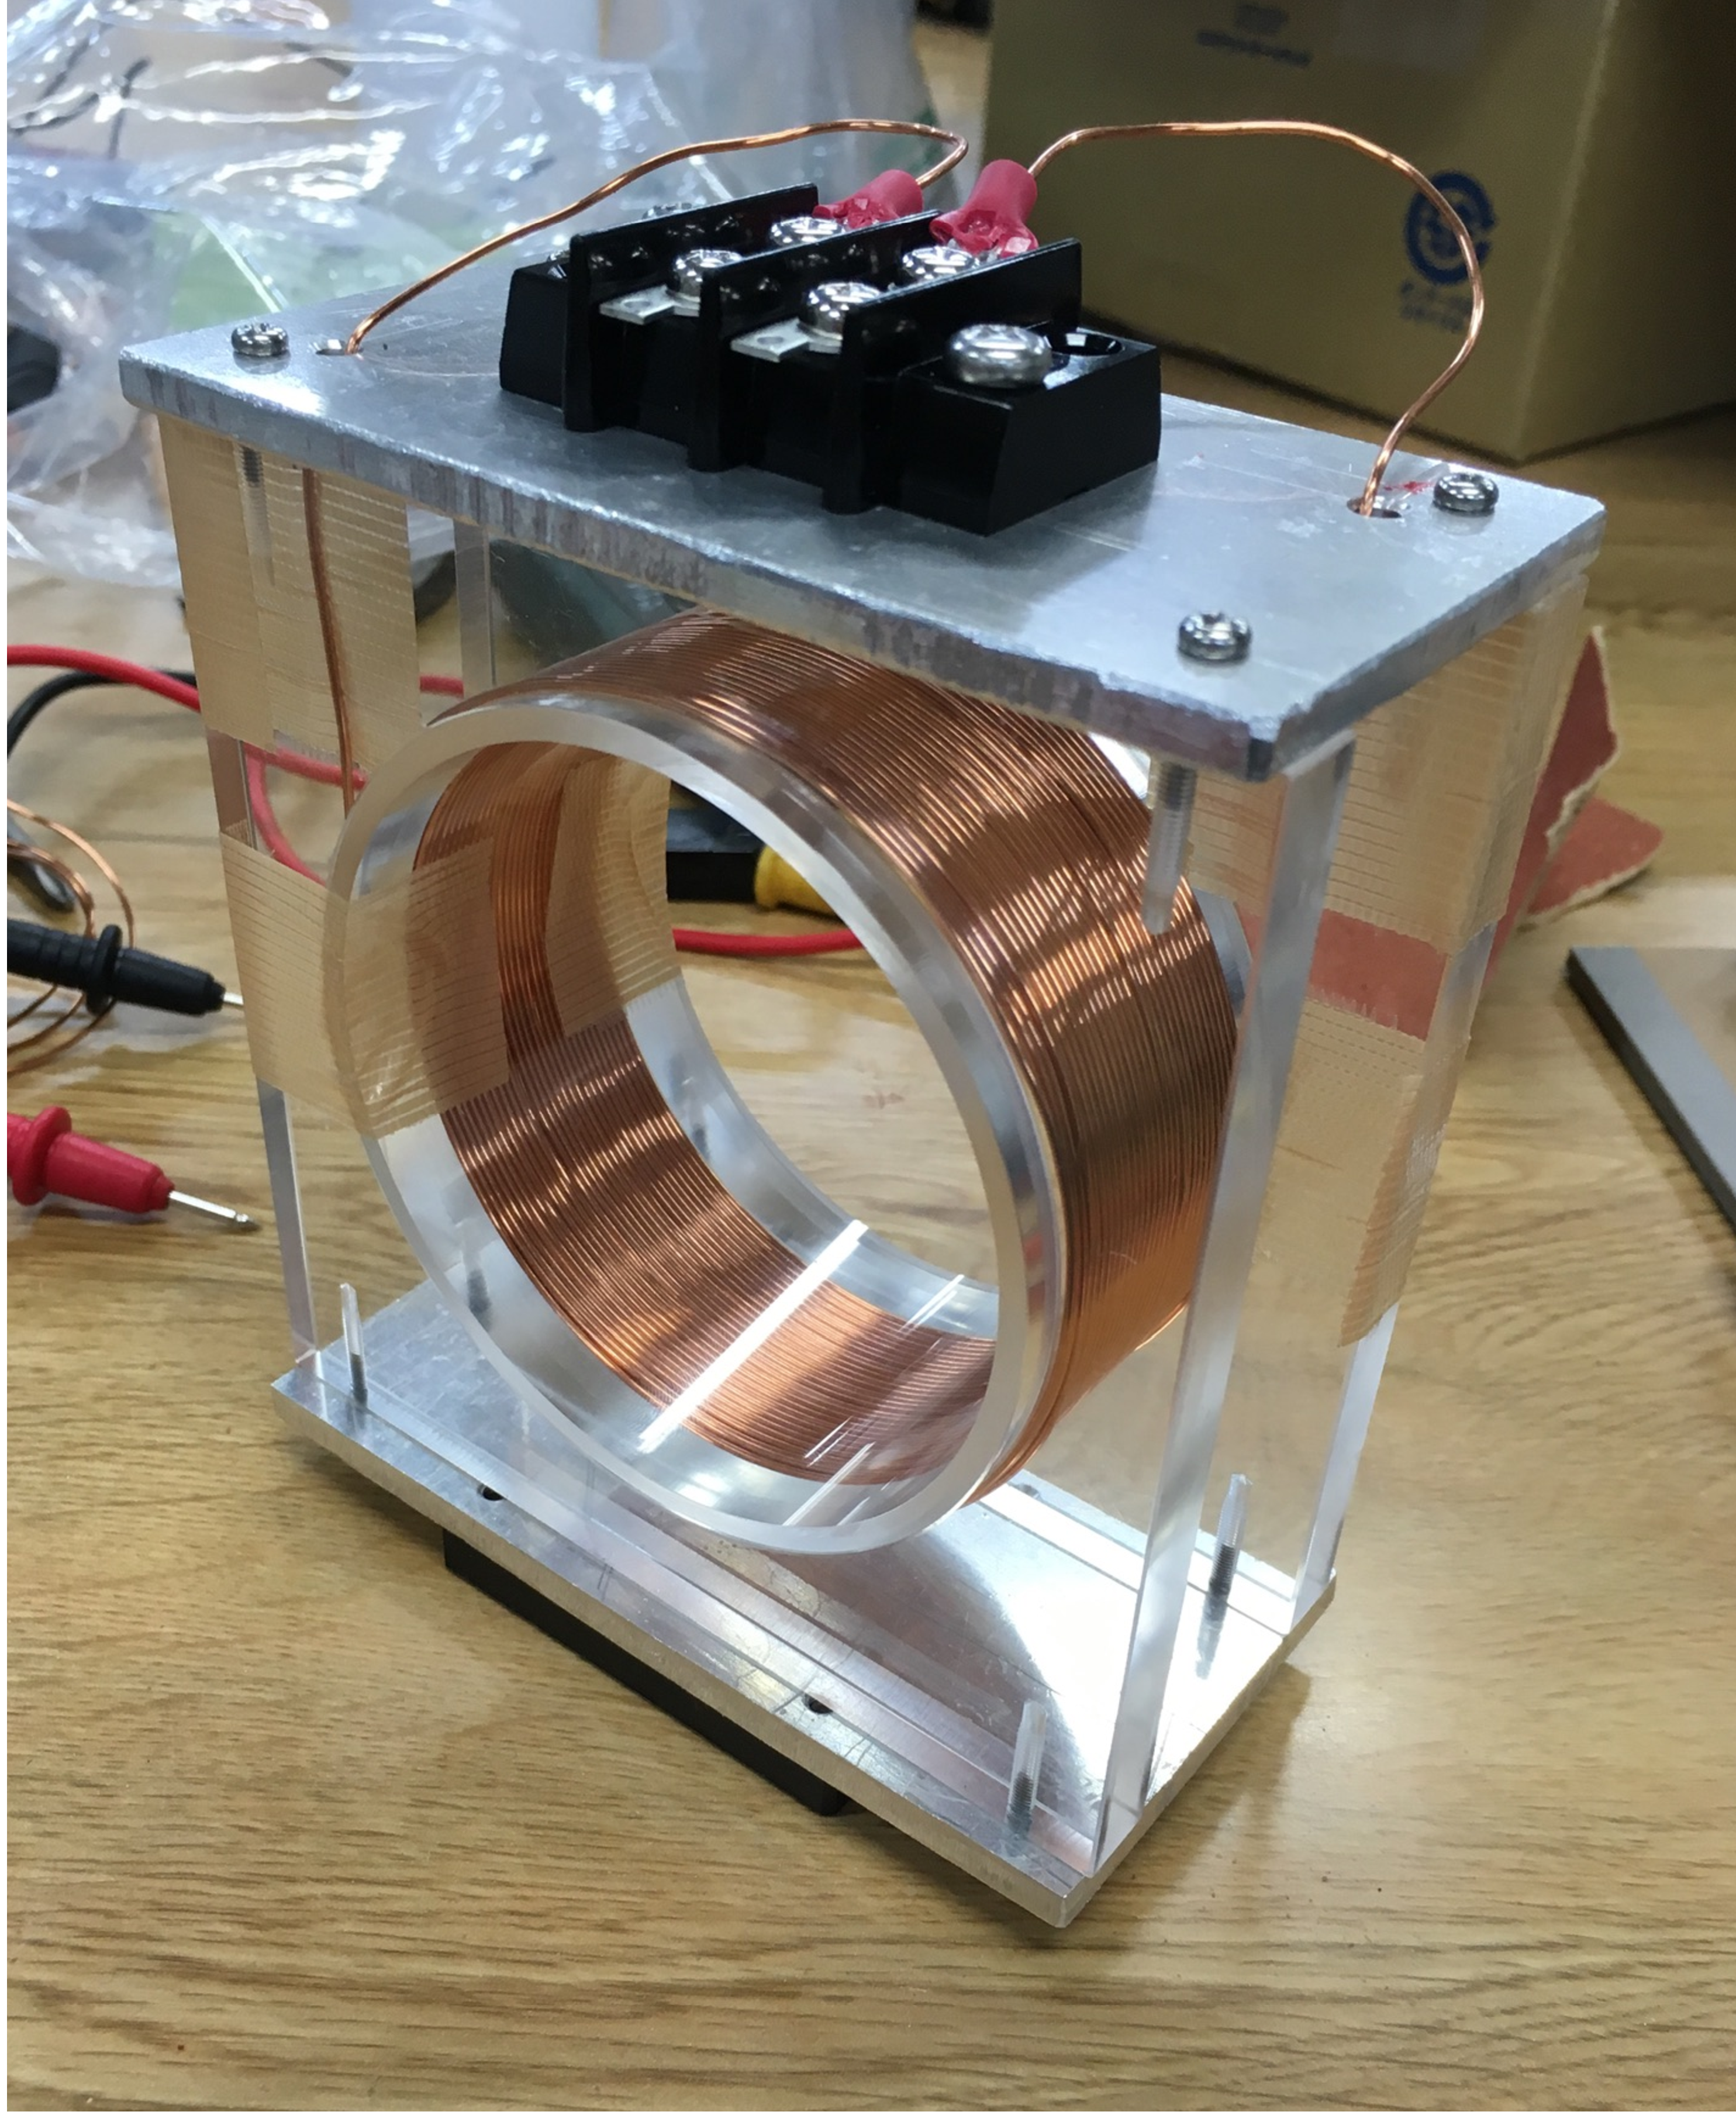
\includegraphics[width=5cm,height=6cm]{device/spinflipperphoto.pdf}\caption{自作したスピンフリッパ―}
\end{center}
\end{figure}
\subsection{位相シフタコイル}
位相シフタコイルの役割は垂直方向に磁場を作り出し、上向きスピンの中性子と下向きスピンの中性子それぞれに位相差を付けることである。\\
フリッパ―と同様にソレノイドコイルに定電流を流すことによって定磁場を作り出している。
\begin{figure}[H]
\begin{center}
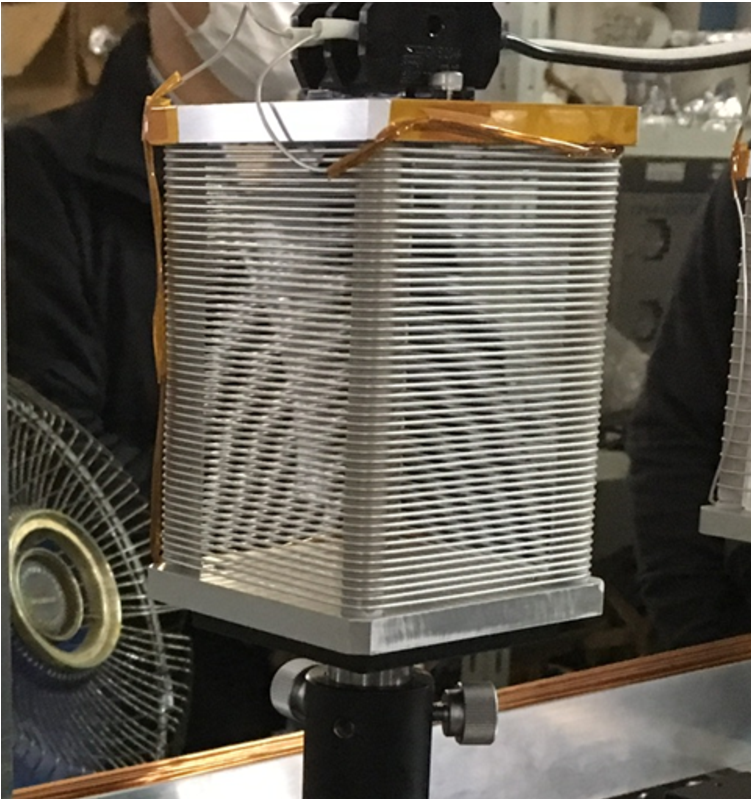
\includegraphics[width=5cm,height=6cm]{device/shifterphoto.pdf}\caption{位相シフタコイル}
\end{center}
\end{figure}
\section{スーパーミラーによるスピンの選択}
\nocite{neutron_spin_optics}
この実験では、特定のスピンを持つ中性子を選択的に取り出す必要がある。この節では、そのために用いるスーパーミラーの原理について説明する。

\subsection{中性子の光学的性質}
\paragraph{屈折率}
中性子が物質中で感じるポテンシャルを$V$とすると、エネルギー保存から
\begin{align}
k^2-k'^2=2mV
\end{align}
となる。$k$は入射中性子の波数、$k'$は物質中での中性子の波数である。
屈折率の定義
\begin{align}
n=\frac{k'}{k}
\end{align}
から、中性子の物質中における屈折率は
\begin{align}
n^2=1-\frac{2mV}{k^2}\label{mirror_neutron_refindex}
\end{align}
となる。

\paragraph{全反射が起きる条件}\label{mirrir_perfect_reflection}
$n-1$が有限の値を持つことは、中性子が全反射しうることを意味する。全反射が起きるための角度の条件は、
臨界角
\begin{align}
\theta^*=\arccos{n}
\end{align}
を用いて
\begin{align}
n\leq\cos\theta^* \label{mirror_refindex_range}
\end{align}
となる。また、全反射が起きるための入射エネルギー$E$の条件は、(\ref{mirror_neutron_refindex}), (\ref{mirror_refindex_range})より
\begin{align}
&n^2=1-\frac{2mV}{k^2}\leq\cos^2\theta^*\\
&E\sin^2\theta\leq E\sin^2\theta^*=\frac{k^2}{2m}\sin^2\theta^*\leq V
\end{align}
となる。すなわち、臨界角以下で入射する時、エネルギーの``ミラーに対し垂直な成分''が$V$よりも小さければ、
全反射が起きることがわかる。

\subsection{磁性体単層膜によるスピンの選択}
磁性体の単層膜を利用することで、特定のスピンを持つ中性子を選択的に取り出すことができる。
中性子が単層膜中で受けるポテンシャルは、核力によるポテンシャル$V_\mathrm{n}$、単層膜中の磁束密度$B$を用いて
\begin{align}
V^{\pm}&=V_\mathrm{n}\pm|\mu_\mathrm{n}|B
\end{align}
となる。$\mu_\mathrm{n}|B|$の符号とスピンの向きの対応は磁場の向きによって決まるが、ここでは上向きスピンのときに正になるものとする。
すなわち、上向きスピンの中性子は$V^+$、下向きスピンの中性子は$V^-$を感じる。

\ref{mirrir_perfect_reflection}節で述べたように、入射中性子のエネルギーを$E$とすると、
\[
E\sin^2\theta\leq V
\]
のときに全反射が起きる。
$V^-< E\sin^2\theta\leq V^+$のエネルギーを持つ中性子をこの単層膜に入射させると、下向きスピンの中性子はほとんどが透過するが、
上向きスピンの中性子は全反射される。$V^+<E\sin^2\theta$の中性子が入射した場合は、上向き、下向き両方の粒子が
透過する確率を持つ。
そのため、透過した中性子には上向きスピンと下向きスピンの両方が含まれる。
$E\sin^2\theta\leq V^-$となるような低エネルギーの中性子は今回の実験では無視できるほど少ないため、
考えなくて良い。

\begin{figure}[h]
\centering
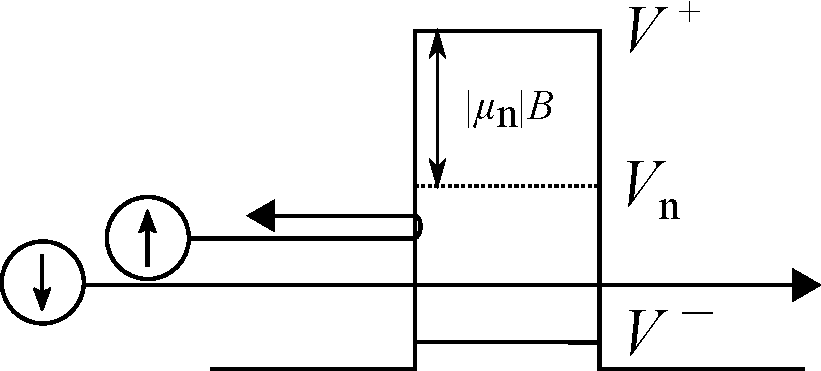
\includegraphics[width=8cm]{mirror/mono_mirror.pdf}
\caption{単層膜によるスピンの選択の原理。実際には、ポテンシャルは紙面奥に向かって2次元に広がっており、
中性子は臨界角以下で入射していることに注意。}
\end{figure}
このようにして、単層膜は上向きスピンの粒子のみを選択的に反射する。

\subsection{スーパーミラー}
\begin{figure}[H]
\centering
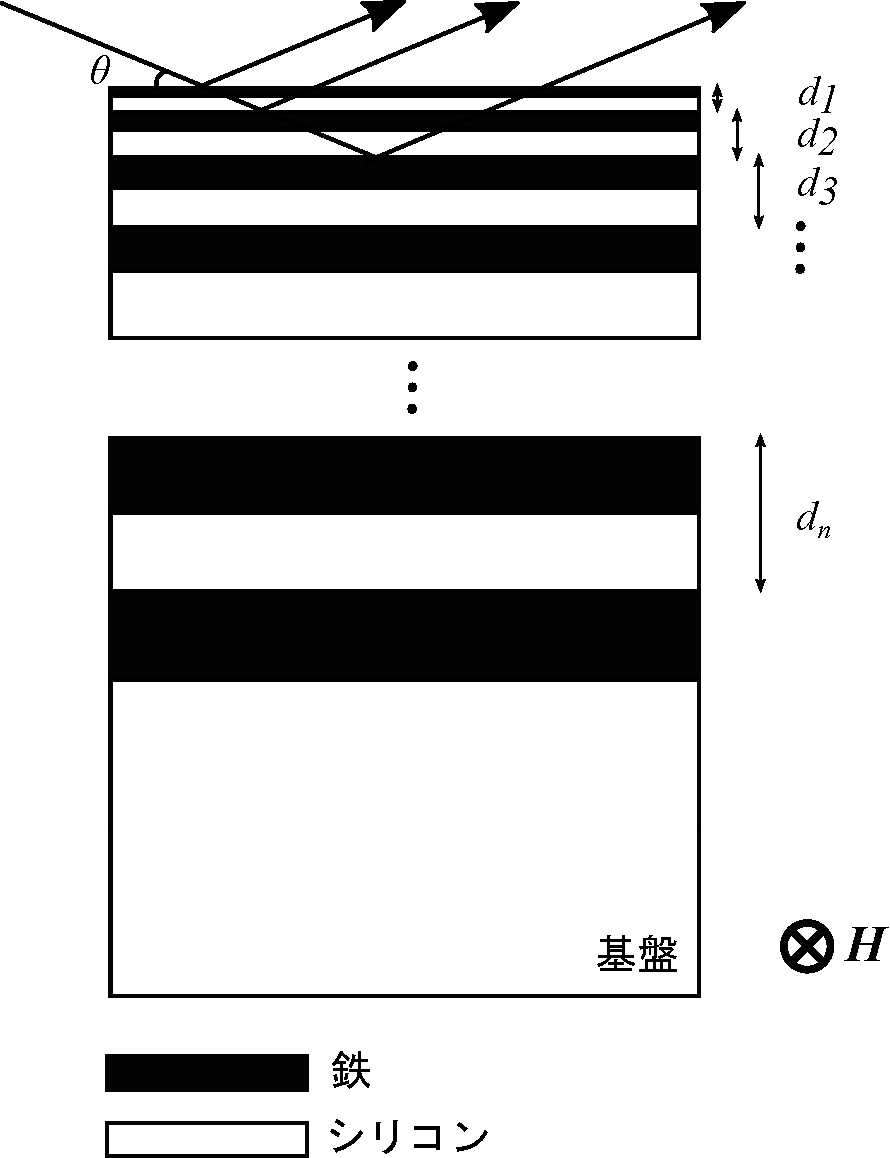
\includegraphics{mirror/super_mirror.pdf}
\caption{スーパーミラーの構造\cite{seki}\label{mirror_super_mirror}}
\end{figure}
\begin{figure}[h]
\centering
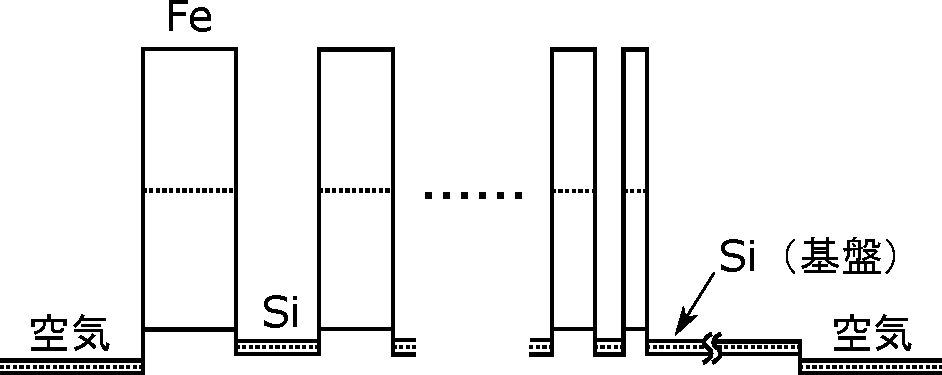
\includegraphics[width=9cm]{mirror/super_mirror_potential.pdf}
\caption{スーパーミラーのポテンシャル。破線は磁場によらない核力によるポテンシャル。実線(上)は上向きスピンの中性子が感じるポテンシャル。
実線(下)は下向きスピンの中性子が感じるポテンシャル。空気やシリコンの透磁率は小さいため、全体に磁場をかけても
ポテンシャルはほとんど影響を受けない。}
\end{figure}
図\ref{mirror_super_mirror}のように膜厚を少しずつ変えた多層膜を使うことで、
単層膜よりも高いエネルギーの中性子を反射するミラーを作ることができる。
これをスーパーミラーと呼ぶ。

\paragraph{Bragg反射による偏極}
$E\sin^2\theta\leq V^+$の中性子は多層膜の表面で全反射されるが、$V^+<E\sin^2\theta$の中性子は多層膜の内部に侵入する。
多層膜の膜間隔を$d$とすると、侵入した中性子はBragg条件
\begin{align}
2d\sin\theta=\lambda
\end{align}
を満たす場合に反射波が強め合う。$\lambda$は中性子の物質波の波長で、
$\lambda=2\pi/k$の関係にある。

$d$を少しずつ変えることで、$V^+<E\sin^2\theta$の様々なエネルギーを持つ上向きスピンの中性子がBragg反射される。
下向きスピンの中性子もわずかに反射されるが、その数は少なく、無視できる。
こうすることで、単層膜に比べより広いエネルギーの中性子のスピンを偏極することができる。

\section{検出器}
中性子は電荷をもたないため、その検出は強い相互作用を通じて行われる。強い相互作用による反応で生じた荷電粒子を検出することで、間接的に中性子を検出する。検出に利用する反応は検出する中性子のエネルギーによって様々であるが、熱中性子($\sim 25$ meV)の場合、次のような中性子捕獲反応が主に利用される:
\begin{align}
&\ce{^3He} + \ce{n} \to \ce{^3H}+\ce{p} + 0.705 \mathrm{MeV} \label{Kasuya_3He} \\
&\ce{^6Li} + \ce{n} \to \ce{^3H}+\ce{^4He}+4.78 \mathrm{MeV} \label{Kasuya_6Li}
\end{align}

\subsection{$\ce{^3He}$ガスを充填した比例計数管}
今回の実験では入射する中性子の時間情報と個数を知る必要がある。そこで入射粒子の数を1つずつ数える微分型の検出器として、$\ce{^3He}$ガスを充填した比例計数管を用いた。

\paragraph{検出原理}
検出には(\ref{Kasuya_3He})の反応が利用される。反応で生じた荷電粒子が気体中を進むと、軌道上の気体分子が電離してイオン・電子対が生じる。電場をかけてそれらを集めることで、信号として読み取ることができる。エネルギー25meVの中性子に対する$\ce{^3He}$原子核の断面積は$5333$barn[]であり、低エネルギーでこの断面積は中性子の速度に反比例することが知られている[]ため、エネルギー$E$(meV)の中性子に対する$\ce{^3He}$原子核の断面積は$\sigma(E)=5333\sqrt{25/E}$(barn)となる。これは気体の中では非常に大きく、効率よく中性子の数を数えることができる。

\paragraph{検出器の仕組み}
円筒形の容器の中に$\ce{^3He}$ガスが封入されており、高電圧がかけられた中心のワイヤと接地された容器の内壁がそれぞれ陽極と陰極として機能する。$\ce{^3He}$ガスは(\ref{Kasuya_3He})の反応によって荷電粒子を発生させる中性子有感物質であると共に、この荷電粒子によって電離して信号を増幅させる被電離気体の役割を果たす。

\begin{figure}[h]
\begin{minipage}{0.5\hsize}
\begin{center}
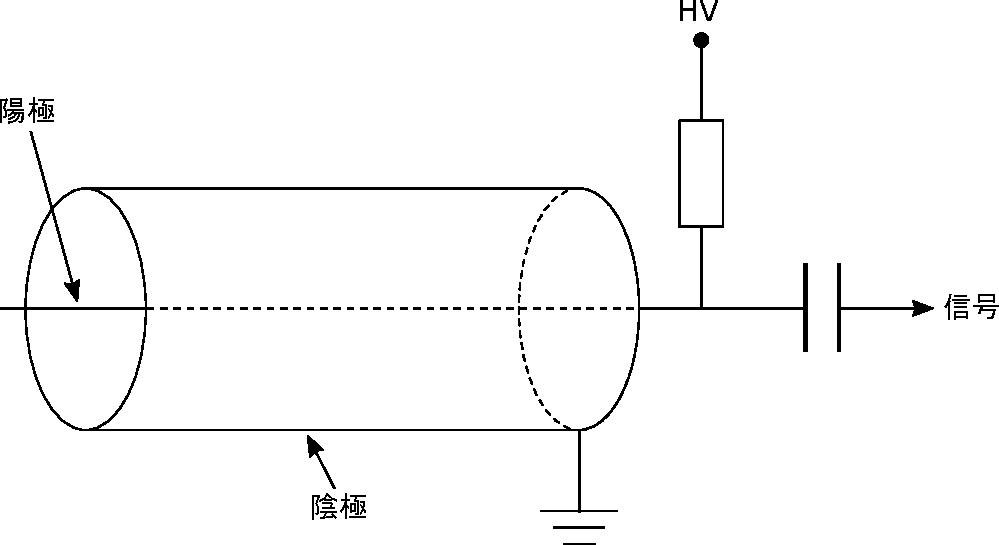
\includegraphics[width=6.5cm]{detector/detector_fig1.pdf}
\caption{比例計数管写真}
\end{center}
\end{minipage}
\begin{minipage}{0.5\hsize}
\begin{center}
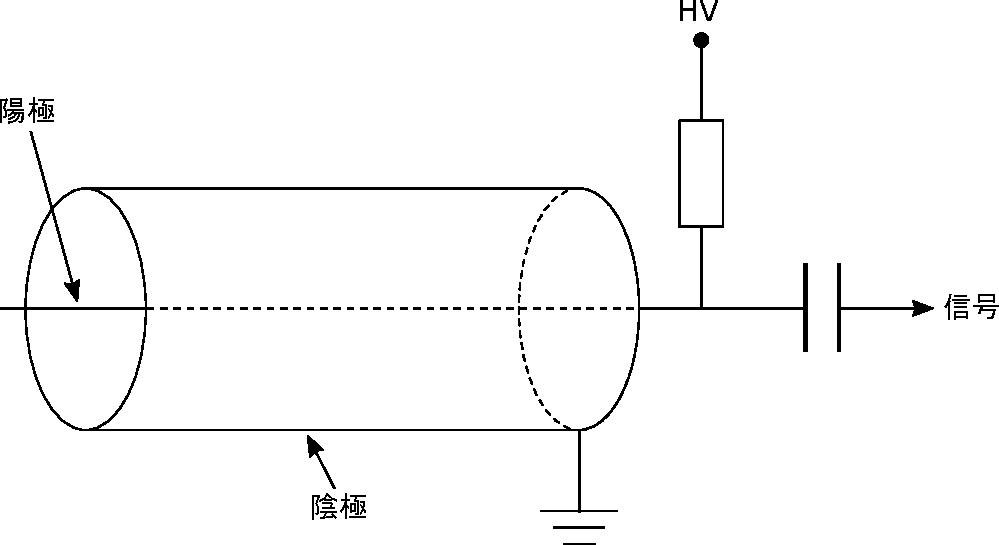
\includegraphics[width=6.5cm]{detector/detector_fig1.pdf}
\caption{比例計数管模式図}
\end{center}
\end{minipage}
\end{figure}

\subsection{RPMT検出器}
予備実験では入射する中性子の2次元的な位置情報を知る必要がある。そこで2次元位置感度型検出器として、RPMT検出器を用いた。

\paragraph{検出原理}
検出には(\ref{Kasuya_6Li})の反応が利用される。反応で生じた荷電粒子によってシンチレータ中の原子や分子が励起され、下の準位に戻る際に光が放出される(シンチレーション光)。生じた光は光電子増倍管で増幅され信号として取り出される。RPMTではシンチレータに$\ce{^6LiF}/\ce{ZnS}$を用いる。$\ce{^6LiF}/\ce{ZnS}$は発光量が大きくガンマ線感度が低いことから、中性子の検出に適している。

\paragraph{検出器の仕組み}
RPMTは$\ce{^6LiF}/\ce{ZnS}$シンチレータにPSPMT(Position Sensitive PMT,位置分解能をもつ光電子増倍管)を取り付けた構造をしている。PSPMTは内部にX軸Y軸のメッシュ状の読み取り用電極をもち、電荷分割法により中性子の検出位置を$x/L=Q_2/(Q_1+Q_2)$で求めることができる。ここで$L$は電極の全長、$x$は検出位置、$Q_1,Q_2$は2本のケーブルからの出力電荷である。検出位置はX軸Y軸について1024ch$\times$1024chの分解能で計測され、チャンネル幅[mm/ch]は$1\mathrm{[ch]}=0.119\pm0.002\mathrm{[mm]}$と報告されている[]。

\begin{figure}[h]
\begin{minipage}{0.5\hsize}
\begin{center}
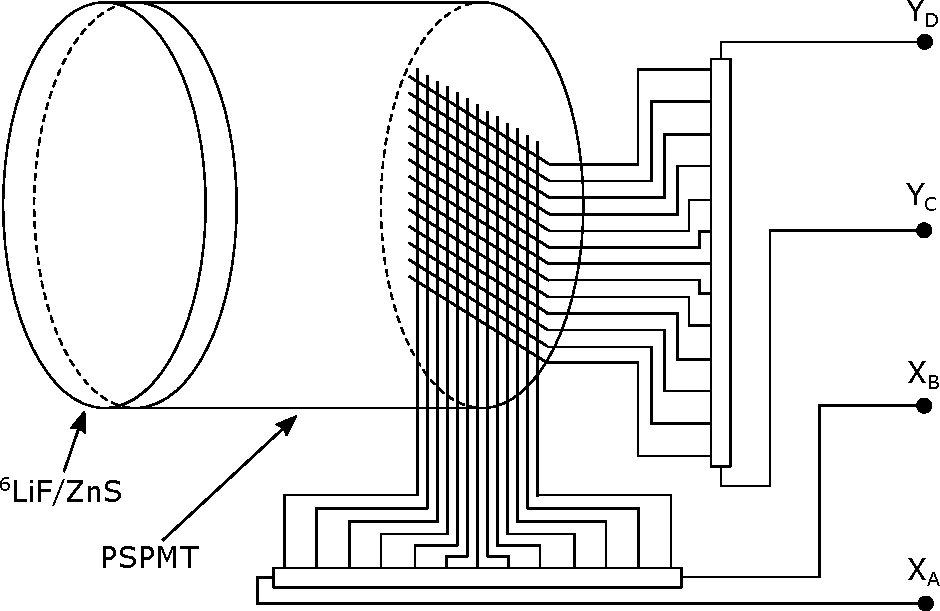
\includegraphics[width=6.5cm]{detector/detector_fig2.pdf}
\caption{RPMT写真}
\end{center}
\end{minipage}
\begin{minipage}{0.5\hsize}
\begin{center}
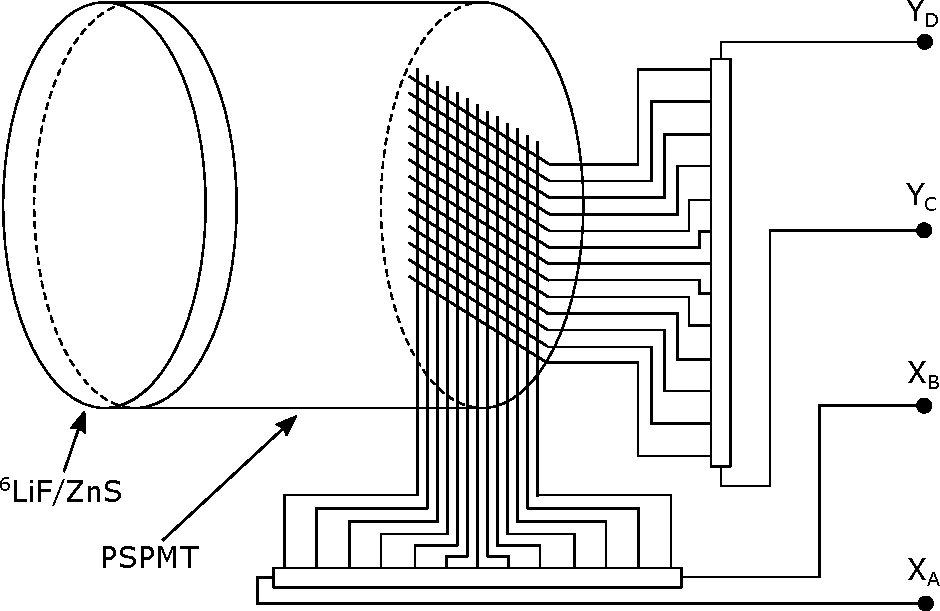
\includegraphics[width=6.5cm]{detector/detector_fig2.pdf}
\caption{RPMT模式図}
\end{center}
\end{minipage}\\
\begin{minipage}{0.5\hsize}
\begin{center}
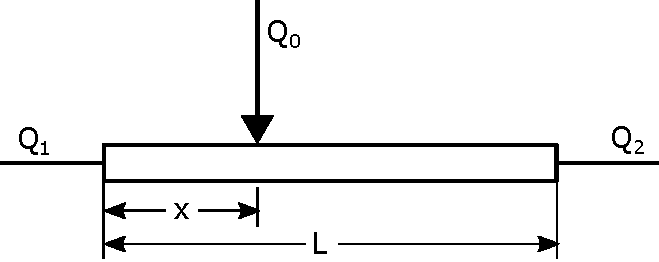
\includegraphics[width=6.5cm]{detector/detector_fig3.pdf}
\caption{電荷分割法}
\end{center}
\end{minipage}
\end{figure}






\section{予備実験:ビーム角度・ミラー角度の最適化}

中性子磁気スーパーミラーは角度1 度未満、波長3  Å以上で入射した中性子しか反射できない。したがって、目的のスピン上向きの中性子を得るためにはミラーで反射した中性子と反射していない中性子を分離する必要がある。以下ではその方法について説明する。

\subsection{最適化の方法}

今回最適化の方法として粒子軌道のシミュレーションを行った。

\begin{figure}[h]
\centering
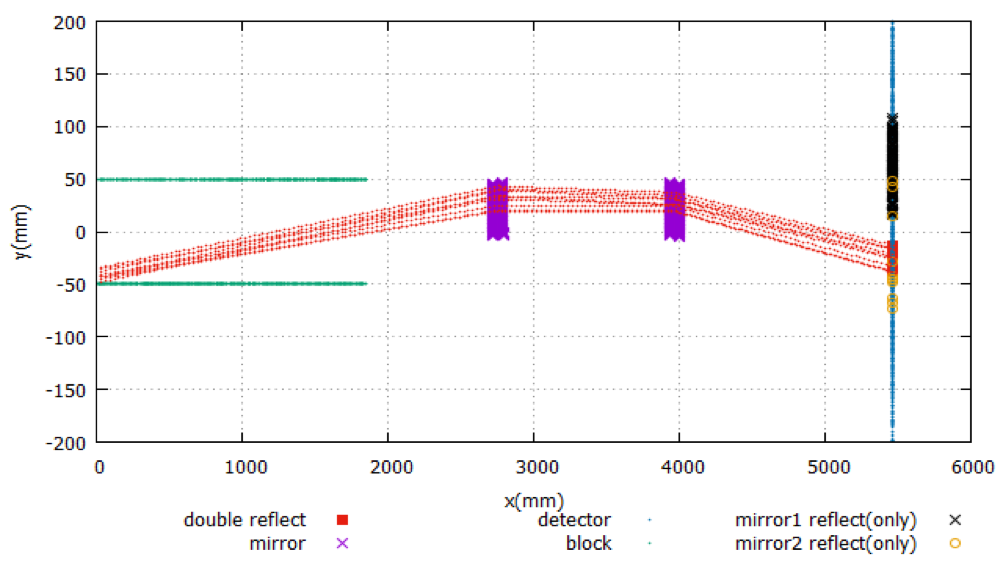
\includegraphics[keepaspectratio,scale=0.4]{angle/simulation.png}
\caption{シミュレーション例}
\end{figure}

これは装置を上から見た図であり、横軸xは粒子の進行方向、縦軸yは粒子の進行方向と垂直な方向を示す。粒子は$x=0$、$y=-50 \sim y=50$の間から角度は一様、エネルギーは予備実験で測定したKUANSのエネルギー分布に従って射出され、 検出器のある場所に到達する。ただし、途中で遮蔽ブロック、あるいはアナライザーに塗ってあるガドリニウムに衝突した場合はその時点で粒子は止まるものとしている。色は、紫はミラーのある位置を意味し、緑はブロックで止まった粒子を表している。また、赤が今回欲しい2回反射した粒子を表しており、他の色の粒子(水色はミラーに反射されなかった中性子、黒はポラライザーでしか反射されなかった中性子、黄色はアナライザーでしか反射されなかった中性子)と区別せねばならない。今回の図は2回反射された中性子を分かりやすくし、どの軌道を主に通るか分かるように軌道を赤色で示してある。

\subsection{コリメータによるビーム角度の最適化}

まず、ポラライザーのみを置いたシミュレーション結果が以下の通りである。(今回はポラライザーで反射した中性子を黒の軌道で表している。)

\begin{figure}[H]
\centering
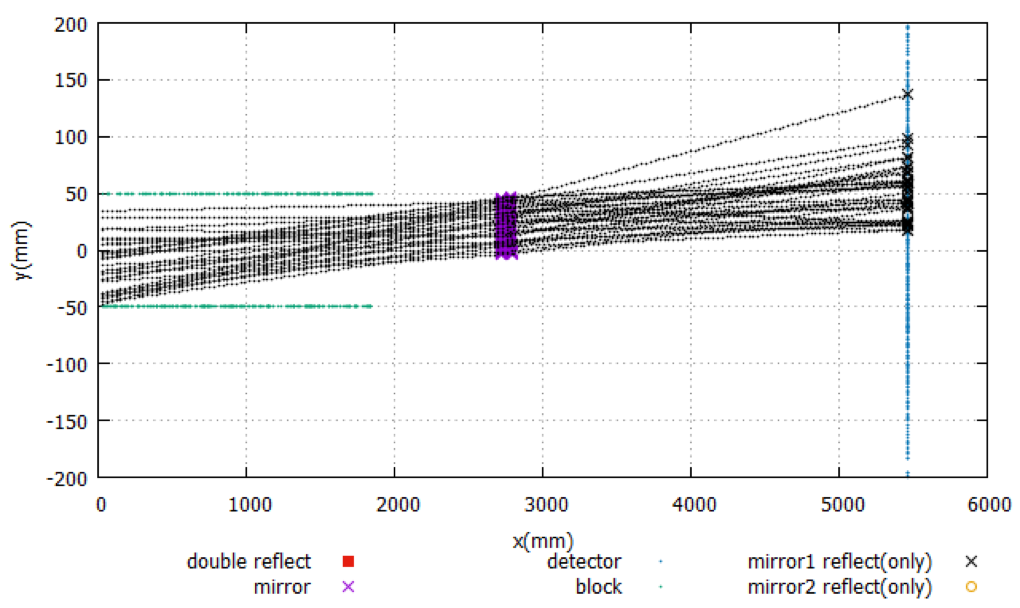
\includegraphics[keepaspectratio,scale=0.4]{angle/nocolimator.png}
\caption{コリメーションをしていない場合}
\end{figure}

今回分離しなければならないのはポラライザーで反射していない水色と、反射した黒を分離することである。しかし、この図でわかるように今の場合分離できておらず重なってしまっている。従って、この2つを分離する操作をする必要がある。今回分離できていない原因の1つとして、ビームが広がり過ぎてしまっていることが挙げられる。そのため、まずコリメーター部分でビーム幅を制限する事を考える。

まず、どの程度ビームを制限するかについてであるが、本実験で使用する$^3$He検出器は大きさが約$20$ mmであり、それ以上のビーム幅を持たせてもあまり意味がない。従って、今回はビーム幅を$20$mmで制限する。また、この$20$mmの幅のビームを$y=-50 \sim y=50$のどこから取り出すかであるが、予備実験の結果からビームは右側から多く射出されることが分かっているので、右側からビームを取り出す。そのため、ビームに$1.46$度の角度をつける。

以上の考察をもとにビームのコリメートをする。今回はビームを制限するためにビームの通過しない箇所をポリエチレンブロックで遮蔽する。その結果が以下の通りである。

\begin{figure}[H]
\centering
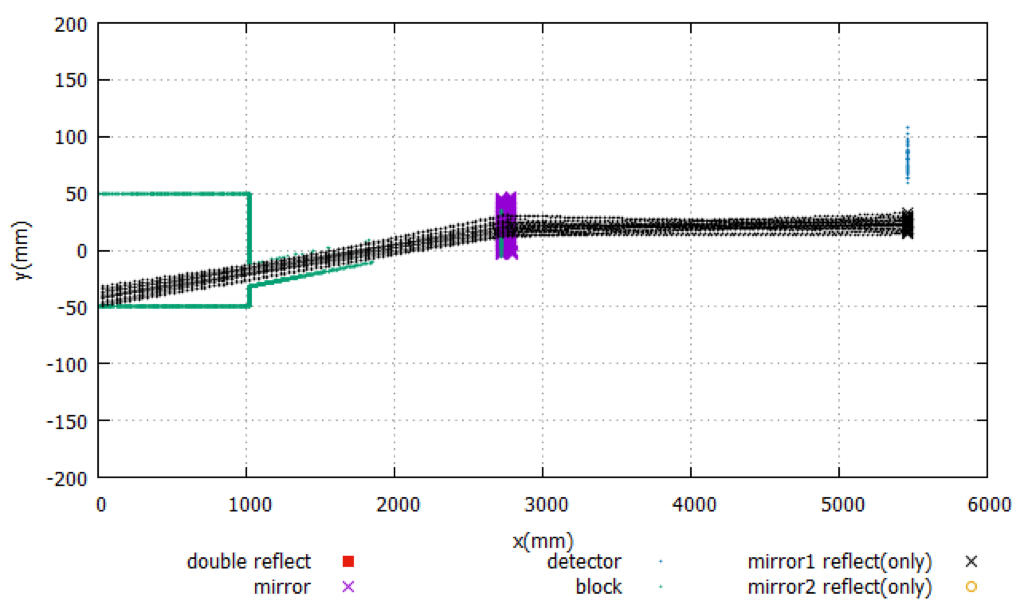
\includegraphics[keepaspectratio,scale=0.4]{angle/colimator.png}
\caption{コリメーションをした場合}
\end{figure}

図から分かるようにビーム幅を制限することによりポラライザーで反射した成分(黒)、反射しなかった成分(水色)を分離する事が出来た。

\subsection{ポラライザー角度の最適化}

次にミラー角度について考察をする。ミラーで反射した中性子と反射していない中性子を分けるにはミラーをビームに対して傾ければ良い。なぜなら、反射せず透過した中性子の軌道はミラーを傾けても変化しない一方、反射した中性子はより大きな角度をつけられて反射するからである。しかし、ミラーをビームに対して傾けすぎると相対角度が1度を超えてしまうため反射しなくなる。したがって、最も適切なミラーの角度を決める必要がある。また、中性子がガイド磁場の中心を通る必要があるため、中性子ビームとガイド磁場コイルとの平行度が高くなるよう考慮した。さらにその中で、反射される中性子が最も多くなるようにした。今回、ポラライザーの角度として$0.87$度、$0.67$度、$0.62$度で実験を行い結果を比較した。シミュレーション結果、PRMTによる実験結果は以下の通りである。ただし、RPMTによる結果はミラーによる反射成分を見やすいように波長3 Å以上の中性子のみに制限している。

\begin{figure}[H]
\begin{minipage}{0.50\hsize}
\begin{center}
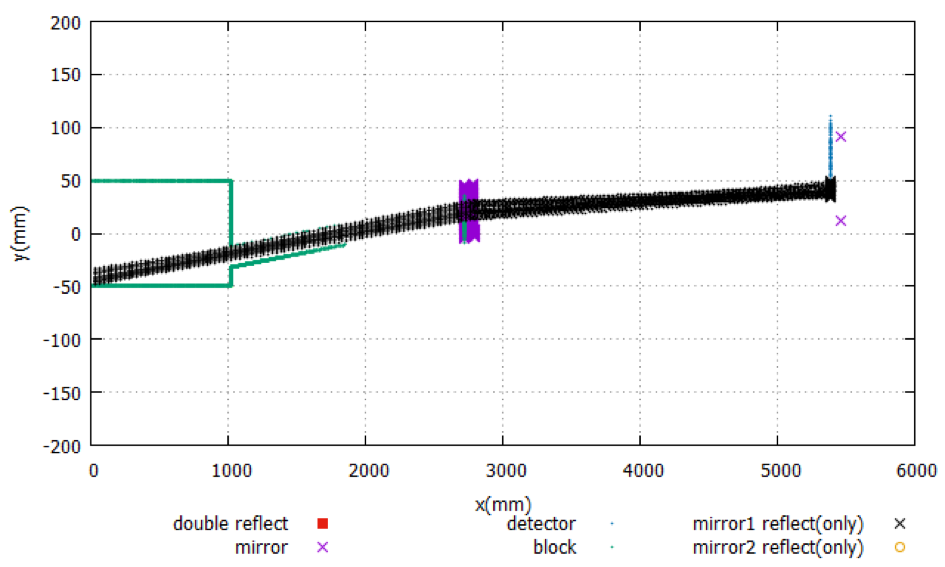
\includegraphics[height=4.5cm]{angle/polonesim.png}
\subcaption{0.87度のシミュレーション}
\end{center}
\end{minipage}
\begin{minipage}{0.50\hsize}
\begin{center}
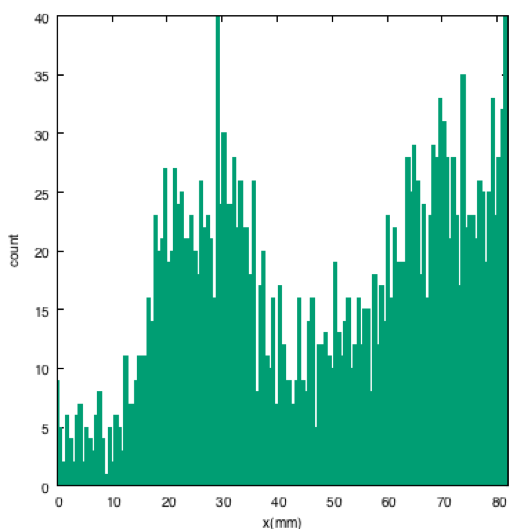
\includegraphics[height=4.5cm]{angle/poloneex.png}
\subcaption{0.87度の実験結果}
\end{center}
\end{minipage}
\caption{0.87度}
\end{figure}

\begin{figure}[H]
\begin{minipage}{0.50\hsize}
\begin{center}
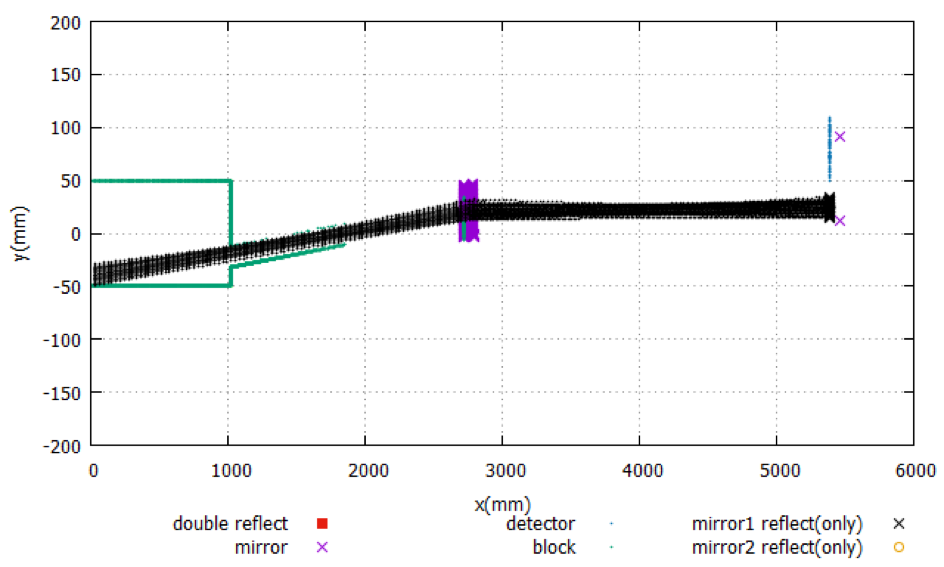
\includegraphics[height=4.5cm]{angle/poltwosim.png}
\subcaption{0.67度のシミュレーション}
\end{center}
\end{minipage}
\begin{minipage}{0.50\hsize}
\begin{center}
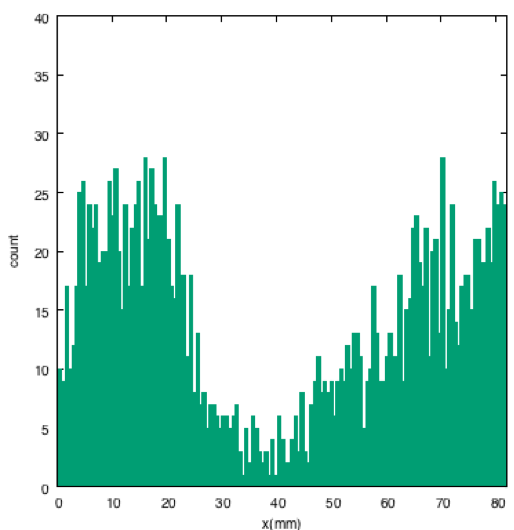
\includegraphics[height=4.5cm]{angle/poltwoex.png}
\subcaption{0.67度の実験結果}
\end{center}
\end{minipage}
\caption{0.67度}
\end{figure}

\begin{figure}[H]
\begin{minipage}{0.50\hsize}
\begin{center}
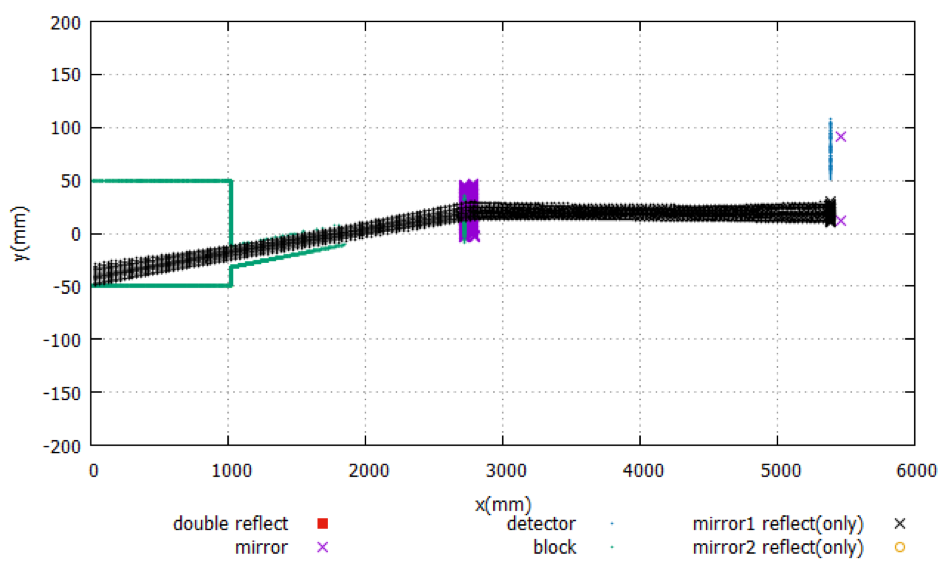
\includegraphics[height=4.5cm]{angle/polthreesim.png}
\subcaption{0.62度のシミュレーション}
\end{center}
\end{minipage}
\begin{minipage}{0.50\hsize}
\begin{center}
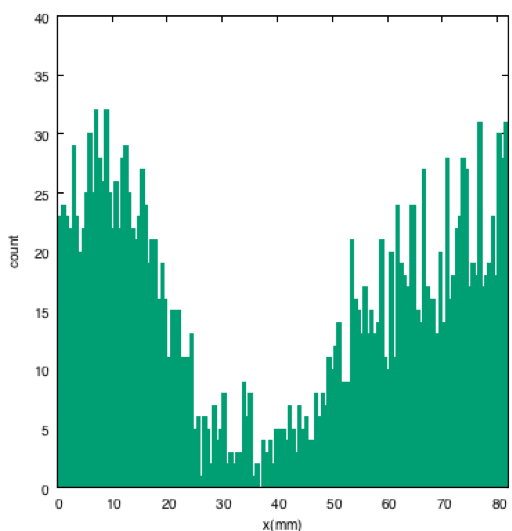
\includegraphics[height=4.5cm]{angle/polthreeex.png}
\subcaption{0.62度の実験結果}
\end{center}
\end{minipage}
\caption{0.62度}
\end{figure}

以上の結果を見ると、ミラーを平行にするほどビームは分離し、どの角度においてもビームが分離できている事がわかる。しかし、$0.87$度では重なってしまっている部分が存在する。また、$0.62$度ではビームがガイド磁場コイルに対して少し傾いてしまっている。したがって、今回はビームが綺麗に分離できており、かつビームがガイド磁場コイルに平行であるという理由からポラライザーの角度を$0.67$度に設定した。

\subsection{アナライザー角度の最適化}

アナライザー角度の設定については、ガイド磁場コイルとの平行度はすでに達成されているので、ミラーに一回反射した中性子と二回反射した中性子の分離、反射される中性子の数の増加の二点を満たすようにアナライザーの角度を設定した。アナライザー角度の設定についてもポラライザー角度の設定と同様に行い、ミラーの角度を$1.03$度に設定した。その結果が以下の通りである。

\begin{figure}[H]
\begin{minipage}{0.50\hsize}
\begin{center}
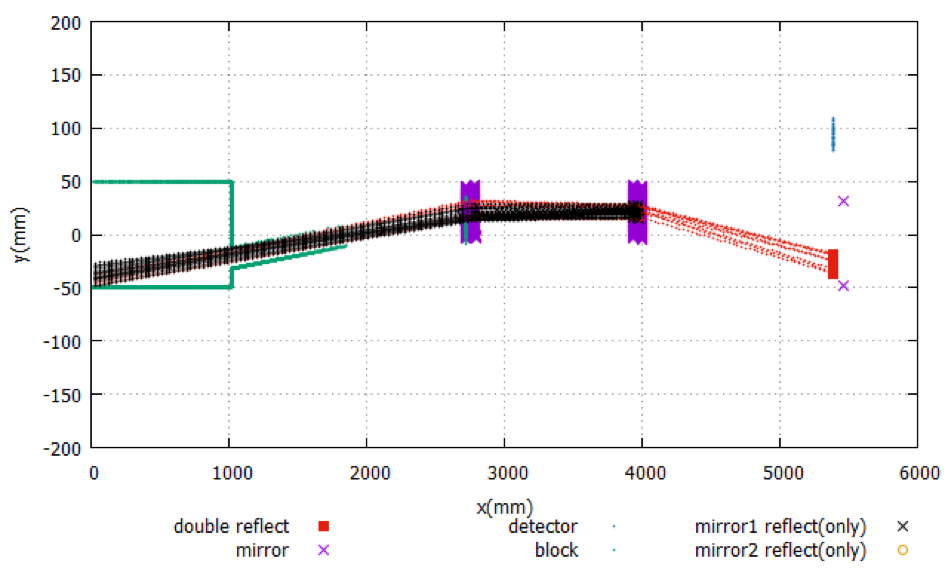
\includegraphics[height=4.5cm]{angle/anaonesim.png}
\subcaption{1.03度のシミュレーション}
\end{center}
\end{minipage}
\begin{minipage}{0.50\hsize}
\begin{center}
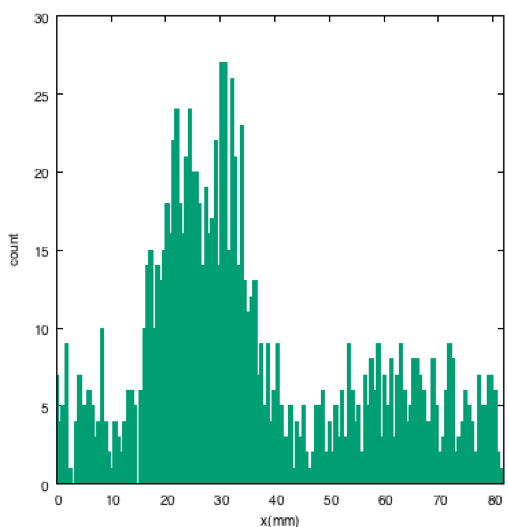
\includegraphics[height=4.5cm]{angle/anaoneex.png}
\subcaption{1.03度の実験結果}
\end{center}
\end{minipage}
\caption{1.03度}
\end{figure}

以上の結果より、ミラーで2回反射された中性子と、その他の中性子を分離する事ができた。

\section{予備実験:スピンフリッパーの共鳴}\label{resonance_sec}

「共鳴」は物理の様々な場所で登場する。例えば音叉の共鳴。固有振動数の等しいふたつの音叉を用意し片方だけを鳴らす。するともう一方もひとりでに鳴り始める。固有振動数の異なる音叉ではこのような現象は起こらない。このように、系がある特定の振動数に対してのみ特異なふるまいをみせる現象を、物理では広く「共鳴」と呼ぶ。

%スピンフリッパーの共鳴とは、フリッパーで特定の周波数の振動磁場をかけたときにフリッパーを通り抜けたある速度の中性子のスピンが完全に反転してしまう現象をいう。本実験における干渉パターンの見えやすさを高めるために、スピンフリッパーの共鳴が必要となる。
ではスピンフリッパーの共鳴とはいったい何だろうか。何のために共鳴させるのだろう。その実現方法は。この章ではそれらについて説明した後、実際の実験で用いた装置と従った手順、得られたデータを示し、最後にデータの分析を行う。

\subsection{What?\ $\sim$スピンフリッパーの共鳴とは何か$\sim$} \label{Resonance_what}
共鳴条件(\ref{pi2flipper_resonance})が満たされるとき、スピンフリッパーは共鳴しているという。その背後にどんな物理的意味が潜んでいるのだろうか。

一様磁場中に理想化されたRFスピンフリッパーがひとつ置かれた状況を考える。系は3つの領域I,II,IIIからなり、全体に$z$方向一様磁場$B_z$が、領域IIに$x$方向振動磁場$2B_r \cos \omega_s t$がかけられている。
\begin{figure}[h]
\centering
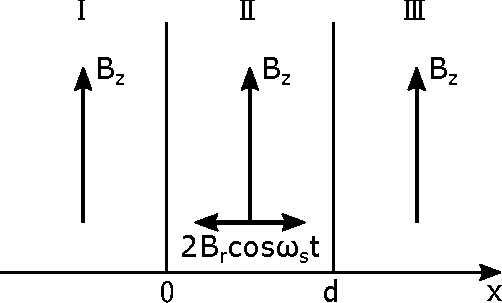
\includegraphics[height=3cm]{resonance/whatwhyhow/Resonance_what_setting.pdf}
\end{figure}

\ref{nonreso_sec}章で述べたように、領域Iからスピン上向きの中性子を入射したとき領域IIIでスピン上向きの中性子を観測する確率は
\begin{equation}
|\psi_{\mathrm{III}}^+|^2=\cos^2 \frac{\omega_A}{v}d+\left(\frac{\epsilon}{\omega_A}\right)^2\sin^2\frac{\omega_A}{v}d \label{Resonance_flip}
\end{equation}
となる。ここで$\epsilon=\omega_s/2-\omega_z,\omega_A=\sqrt{\epsilon^2+\omega_r^2}$であり、$\omega_z=|\mu_n|B_z,\omega_r=|\mu_n|B_r$、$\mu_n$は中性子の磁気モーメント、$d$は領域IIの幅である。

いま$\epsilon/|\omega_z|=0,0.3,0.5,1.0$の各場合についてスピンフリッパーを通過した中性子のスピン反転率($=1-|\psi_\mathrm{III}^+|^2$)と$\omega_r d/v$の関係を図\ref{Resonance_fig_reversalrate}に表す。
図\ref{Resonance_fig_reversalrate}より
\begin{equation}
\epsilon=\frac{\omega_s}{2}-\omega_z=0 \label{Resonance_resonance}
\end{equation}
がなりたてば、
\begin{equation}
\frac{\omega_r}{v}d =\frac{(2n+1)\pi}{2} \quad (n =0,1,2,\cdots) \label{Resonance_piflip_r}
\end{equation}
を満たす速度の中性子に対して、領域IIIにおけるスピン上向き粒子の存在確率が0、すなわちスピン反転率が1になることがわかる。逆に$\epsilon \neq 0$のときはどのような速度の中性子に対しても反転率は1となり得ない。このように、式(\ref{Resonance_resonance})を満たす周波数の振動磁場をかけたときに限りスピンフリッパーを通り抜けた中性子のスピンが完全に反転し得る。これをスピンフリッパーの共鳴と呼び、式(\ref{Resonance_resonance})を共鳴条件と呼ぶ。また速度に対する条件(\ref{Resonance_piflip_r})を$\pi$フリップ条件と呼ぶ。
\begin{figure}[h]
\begin{center}
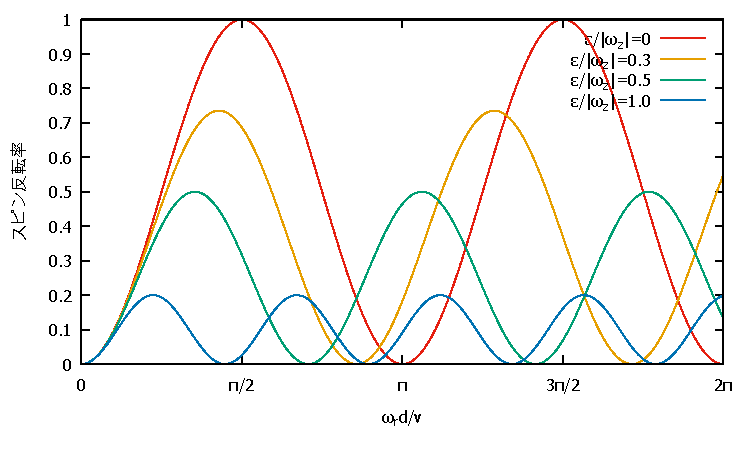
\includegraphics[width=9.5cm]{resonance/whatwhyhow/resonance_reversalrate.pdf}
\caption{スピン反転率}
\label{Resonance_fig_reversalrate}
\end{center}
\vspace{-1cm}
\end{figure}

\subsection{Why?\ $\sim$スピンフリッパーの共鳴はなぜ必要か$\sim$}
スピンフリッパーの共鳴は本実験での干渉がはっきり見えるかどうかの鍵を握っている。ここではスピンフリッパー共鳴の重要性が明らかとなる。

一様磁場中に、理想化されたRFスピンフリッパーふたつとシフタコイルひとつが置かれた状況を考える。系は7つの領域I,II,III,IV,V,VI,VIIからなり、全体に$z$方向一様磁場$B_z$がかけられ、それに加えて領域II,VIに$x$方向振動磁場$2B_r\cos\omega_s t$が、領域IVに$z$方向一様磁場$B$がかけられている。
\begin{figure}[h]
\centering
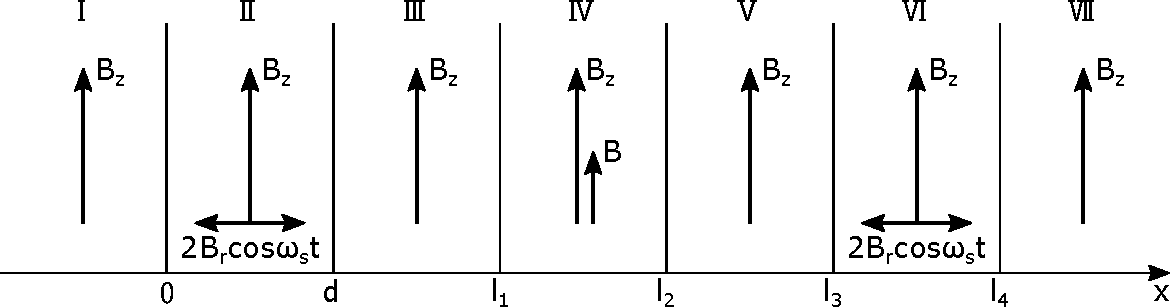
\includegraphics[height=3cm]{resonance/whatwhyhow/Resonance_why_setting.pdf}
\end{figure}

\ref{nonreso_sec}章で述べたように、スピン上向きの中性子が領域Iから入射し、領域I$\sim$VIを通って領域VIIに抜けるとき、領域VIIにおいてスピン上向き中性子を観測する確率は、共鳴からのずれを表すパラメータ$\epsilon$と中性子の速度$v$に依存した係数$N_1,N_2,N_3$を用いて
\begin{equation}
I=N_1-N_2\cos\left(\frac{2}{v}(\omega d'-\epsilon L')\right) -N_3\sin\left(\frac{2}{v}(\omega d'-\epsilon L')\right)
\end{equation}
と表せる。ここで$\omega$は位相シフタコイルの磁場$B$を用いて$\omega=|\mu_n|B$と表される量であり、$d',L'$はそれぞれ位相シフタコイルの幅、2つのスピンフリッパー間距離である。さらに$N_4=\sqrt{N_2^2+N_3^2}$として
\begin{equation}
\cos \phi=\frac{N_2}{N_4}, \quad \sin \phi=\frac{N_3}{N_4}
\end{equation}
で$\phi$を定義すれば、干渉パターンは
\begin{equation}
I=N_1-N_4\cos\left(\frac{2}{v}(\omega d'-\epsilon L')-\phi\right)\label{Resonance_interference}
\end{equation}
と書き直される。

いま、ある$\epsilon$に対して、シフタコイルの磁場を変えながら領域VIIでのスピン上向き中性子の数を計測すると式(\ref{Resonance_interference})の干渉パターンが得られるが、その見えやすさ(ビジビリティ)は$\epsilon$によって異なる。例えば$N_4/N1=1$のときは振幅の大きなはっきりとした(ビジビリティの高い)干渉パターンが得られるが、$N_4/N_1 \ll 1$のときは干渉パターンはほとんど観測できない(ビジビリティが低い)。そこでビジビリティを表す指標$V$を
\begin{equation}
V=\frac{N_4}{N_1}
\end{equation}
で定義すると、$0 \le V \le 1$であり、$V$が大きい程ビジビリティが高い。

いま$\epsilon/|\omega_z|=0,0.3,0.5,1.0$の各場合について干渉パターンのビジビリティ$V$と$\omega_r d/v$の関係を図\ref{Resonance_fig_visivility}に表す。図\ref{Resonance_fig_visivility}より共鳴条件(\ref{Resonance_resonance})がなりたてば、
\begin{equation}
\frac{\omega_r }{v}d =\frac{(2n+1)\pi}{4} \quad (n =0,1,2,\cdots) \label{Resonance_pi2flip_r}
\end{equation}
を満たす速度の中性子に対して、干渉パターンのビジビリティ$V=1$になることがわかる。逆に$\epsilon \neq 0$のときはどのような速度の中性子に対してもビジビリティは1となり得ない。この速度に対する条件(\ref{Resonance_pi2flip_r})を$\pi/2$フリップ条件と呼ぶ。実際、$\omega_rd/v=\pi/4$,$\epsilon/|\omega_z|=0,0.3,0.5,1.0$のときの干渉パターンは図\ref{Resonance_fig_interference}のようになる。すなわちスピンフリッパーを共鳴させる目的は、本実験で得られる干渉パターンのビジビリティを高めるためである。

\begin{figure}[h]
\vspace{-2mm}
\begin{center}
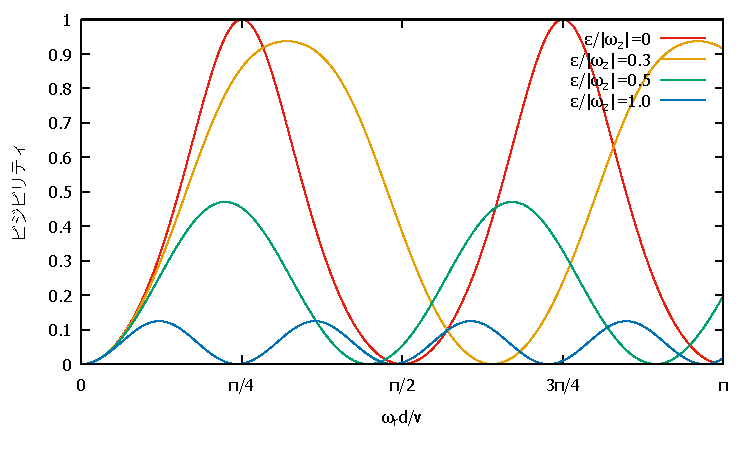
\includegraphics[width=9.5cm]{resonance/whatwhyhow/resonance_visivility1.pdf}
\caption{ビジビリティ}
\label{Resonance_fig_visivility}
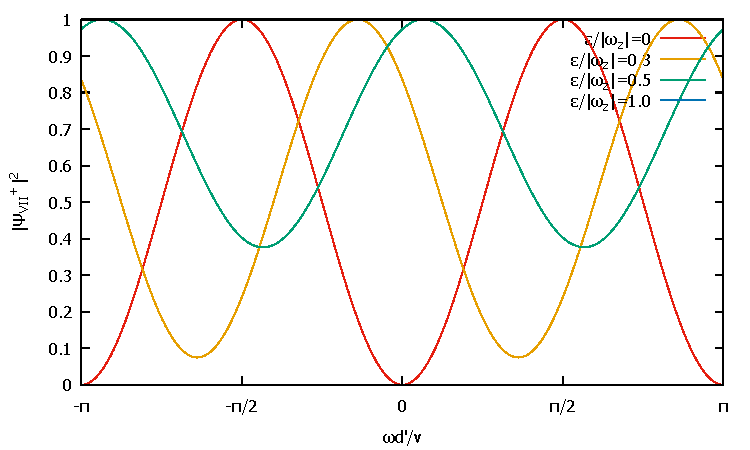
\includegraphics[width=9.5cm]{resonance/whatwhyhow/resonance_interference1.pdf}
\caption{干渉パターン}
\label{Resonance_fig_interference}
\end{center}
\vspace{-1cm}
\end{figure}



\clearpage
\subsection{How?\ $\sim$スピンフリッパーを共鳴させるには$\sim$}
実際にスピンフリッパーを共鳴させるにはどうしたらよいだろう。ここではその実現方法を考え、実際に実験で用いた装置と従った手順を紹介する。

\paragraph{実現方法}
\ref{Resonance_what}節と同じく、一様磁場中にスピンフリッパーがひとつ置かれており、スピン上向き中性子を領域Iから入射させる場合を考える。このとき領域IIIでスピン上向き中性子を観測する確率は式(\ref{Resonance_flip})より
\begin{equation}
|\psi_\mathrm{III}^+|^2 =\cos^2 \frac{\omega_A}{v}d+\left(\frac{\epsilon}{\omega_A}\right)^2\sin^2\frac{\omega_A}{v}d
\end{equation}
であらわされる。これを$\omega_r/|\omega_z|=0.5$のときに、$\epsilon/|\omega_z|=0,0.3,0.5,1.0$の各場合について$\omega_r d/v$に対して図示すると図\ref{Resonance_fig_1-reversal}のようになる。図\ref{Resonance_fig_1-reversal}より、領域IIIでスピン上向き中性子を観測する確率の、速度に対する最小値は共鳴条件(\ref{Resonance_resonance})
を満たすとき最も小さくなり、理想的にはゼロとなることがわかる。共鳴条件を満たすときにスピンフリッパーを通り抜けた中性子のスピン反転率が$1,1/2$となるための中性子の速度に対する条件をそれぞれ$\pi$フリップ条件(\ref{Resonance_piflip})、$\pi/2$フリップ条件(\ref{Resonance_pi2flip})と呼んだが、今回の実験で用いた中性子の速度範囲ではそれぞれ$n=0$の場合のみが満たされ得るので、以後
\begin{equation}
\frac{\omega_r}{v}d=\frac{\pi}{2}\label{Resonance_piflip}
\end{equation}
を$\pi$フリップ条件
\begin{equation}
\frac{\omega_r}{v}d=\frac{\pi}{4}\label{Resonance_pi2flip}
\end{equation}
を$\pi/2$フリップ条件と呼ぶことにする。
\begin{figure}[h]
\begin{center}
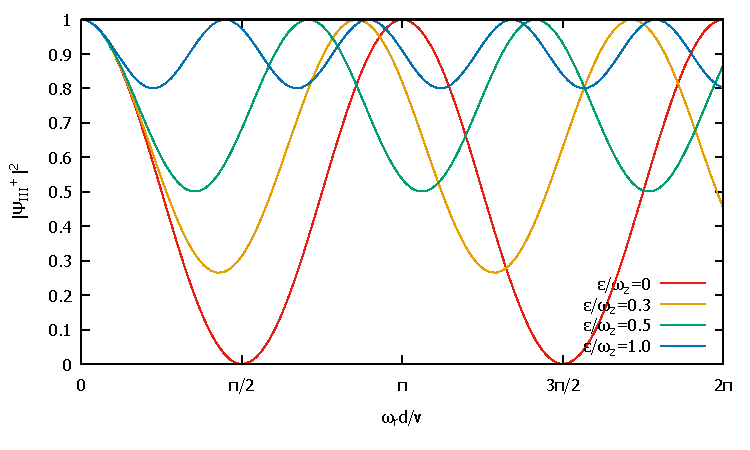
\includegraphics[width=9.5cm]{resonance/whatwhyhow/resonance_1-reversal.pdf}
\caption{$1-反転率$}
\label{Resonance_fig_1-reversal}
\end{center}
\end{figure}

すなわち次のようにして、実験的にスピンフリッパーの共鳴を実現することができる。
\begin{enumerate}
\item スピンフリッパーにスピン上向き中性子を入射し、フリッパーの後ろでスピン上向き成分のみを観測する。
\item 共鳴条件(\ref{Resonance_resonance})が満たされていないと、ある速度の中性子についてはカウントをより減らすことができる。
\item 共鳴条件(\ref{Resonance_resonance})が満たされていると、$\pi$フリップ条件(\ref{Resonance_piflip})を満たす速度の中性子についてはスピンが完全に反転するため、その速度の中性子のカウントは最小となる。
\item カウント分布を見ながら共鳴条件(\ref{Resonance_resonance})に関するパラメータを調節し、カウントが最小となるところを探す。
\end{enumerate}


\paragraph{実験装置}
上流側、下流側それぞれのスピンフリッパーに対して共鳴実験を行った。用いた装置は
\vspace{5mm}
\begin{minipage}{0.5\hsize}
\begin{enumerate}
\item 上流側スピンフリッパー共鳴実験
\begin{enumerate}
\item ガイド磁場コイル
\item 上流側中性子磁気スーパーミラー
\item[(c1)] 上流側スピンフリッパー
\setcounter{enumii}{3}
\item 下流側中性子磁気スーパーミラー
\item \ce{^3He}ガスを充填した比例計数管
\end{enumerate}
\end{enumerate}
\end{minipage}
\begin{minipage}{0.5\hsize}
\begin{enumerate}
\setcounter{enumi}{1}
%\renewcommand{\labelenumi}{}
\item 下流側スピンフリッパー共鳴実験
\begin{enumerate}
\item ガイド磁場コイル
\item 上流側中性子磁気スーパーミラー
%\renewcommand{\labelenumi}{(\alph{enumi} {2})}
\item[(c2)] 下流側スピンフリッパー
\setcounter{enumii}{3}
%\renewcommand{\labelenumi}{(\alph{enumi})}
\item 下流側中性子磁気スーパーミラー
\item \ce{^3He}ガスを充填した比例計数管
\end{enumerate}
\end{enumerate}
\end{minipage}
\vspace{5mm}

また、回路系には次の機器を用い、図のように接続した。
\begin{enumerate}
\renewcommand{\labelenumi}{(\roman{enumi})}
\item 直流安定化電源PWX750MLF(KIKUSUI) $\times 3$ \ \ (以後、直流電源1,2,3)
\item マルチファンクションジェネレータWF1974(エヌエフ回路設計ブロック) \ \ (以後、FG)
\item 1MHzバイポーラ電源HSA4014(エヌエフ回路設計ブロック) $\times 2$ \ \ (以後、アンプ1,2)
\end{enumerate}

\vspace{5mm}
\begin{figure}[h]
\centering
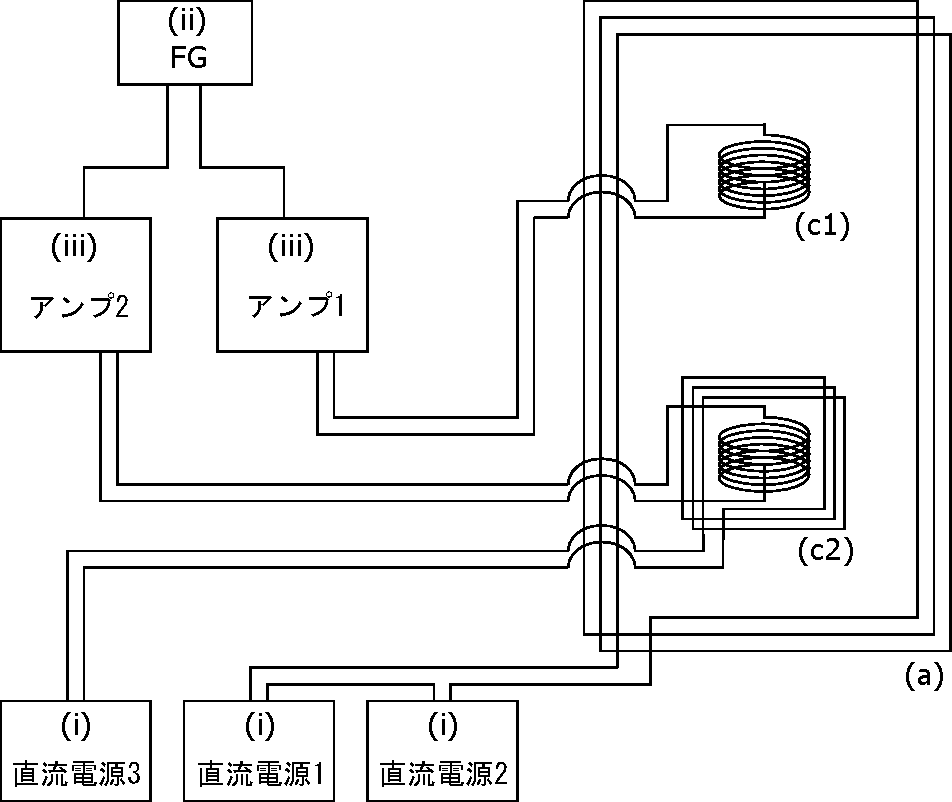
\includegraphics[width=12cm]{resonance/whatwhyhow/kairozu.pdf}
\caption{配線図}
\vspace{-5mm}
\end{figure}

\clearpage
\paragraph{実験手順}
実験は次のフローチャートに沿って行った。
\begin{figure}[h]
\centering
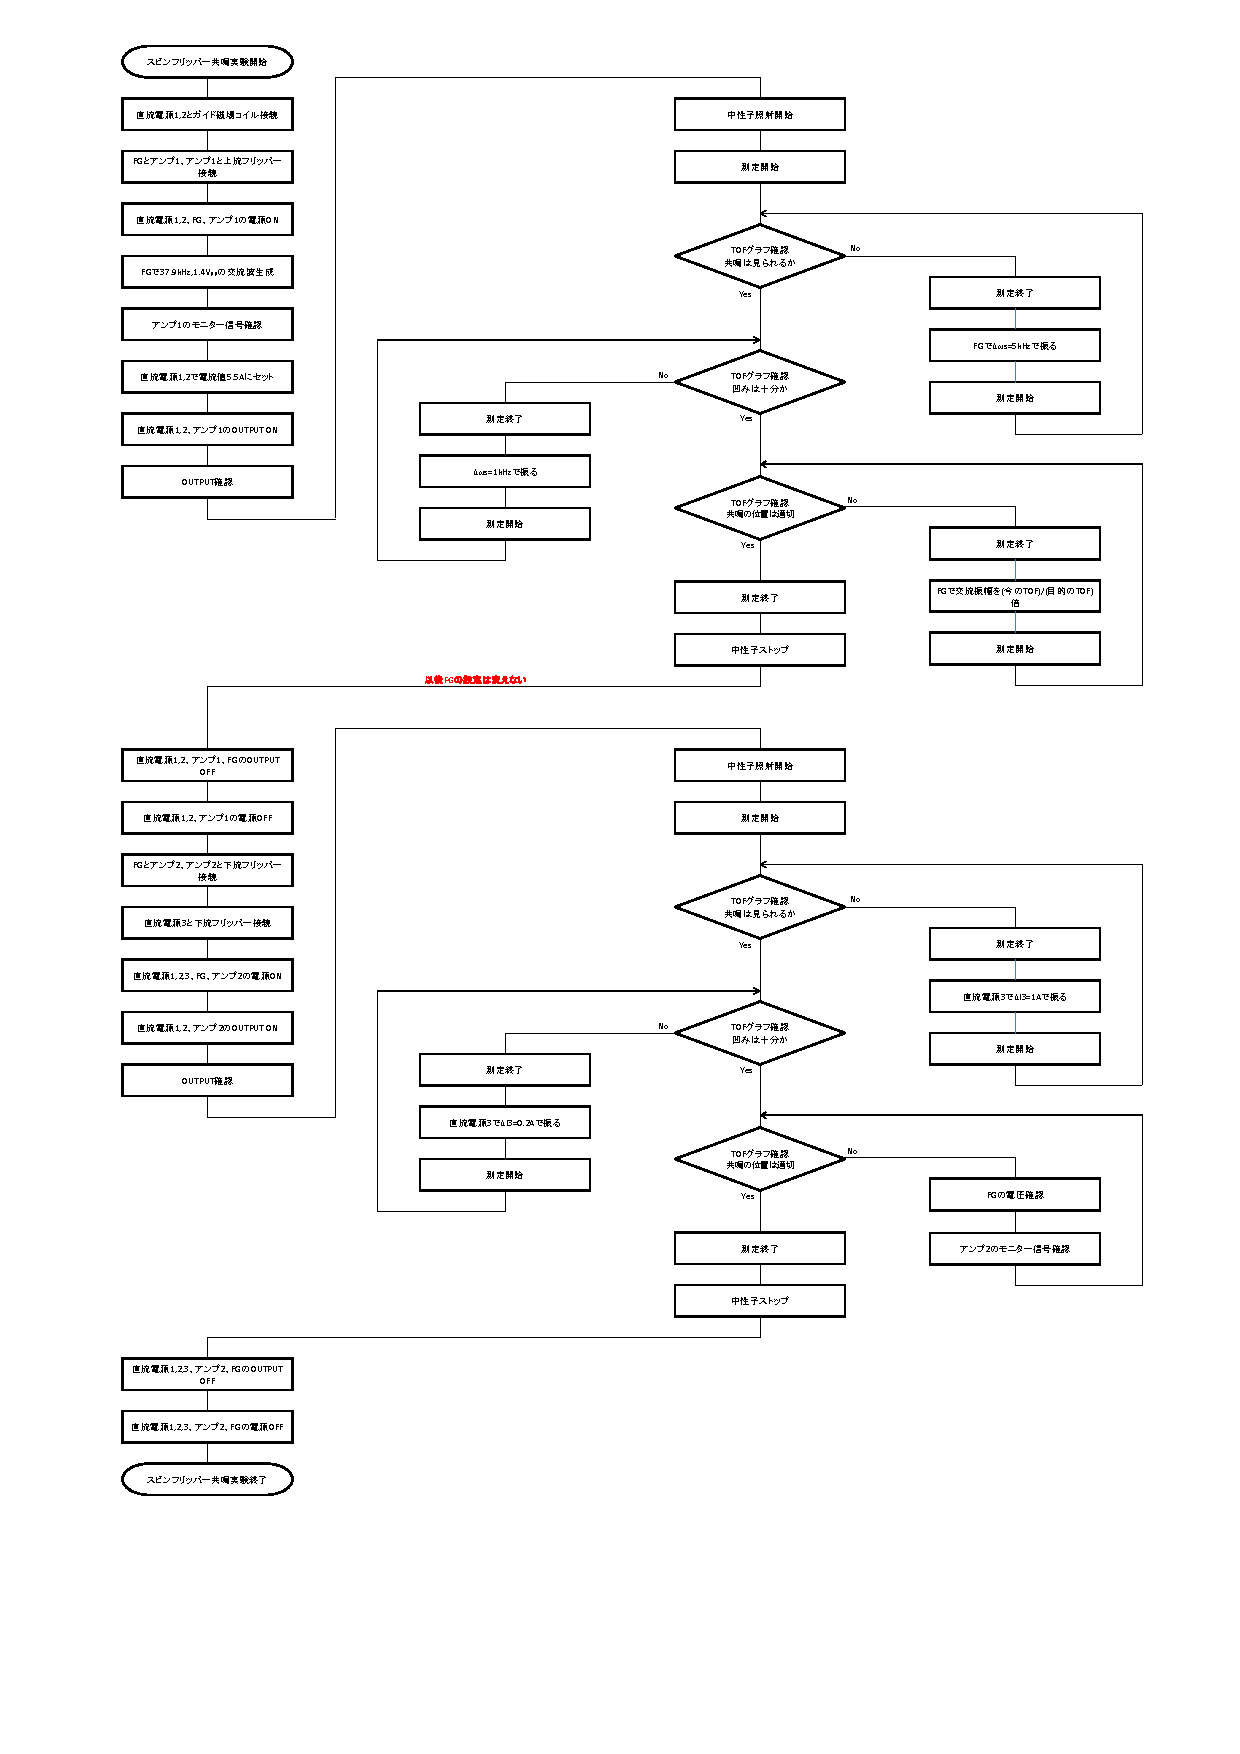
\includegraphics[width=\hsize]{resonance/whatwhyhow/Resonance_flow.pdf}
\vspace{-3.5cm}
\end{figure}

\newpage
次は実際の実験手順である。
\begin{enumerate}
%\renewcommand{\labelenumi}{\arabic{enumi})}
\item (2017.2.22)装置、機器を図のとおりに配置、接続し、上流フリッパー共鳴実験を開始した。
\item 直流電源1,2でガイド磁場コイルに5.5Aの電流を流した。
\item FGで周波数$37.9\, \mathrm{kHz},振幅14.0\, \mathrm{V_{pp}}$の交流波を生成し、アンプ1で増幅して上流フリッパーに交流電流を流した。
\item 中性子の照射を開始した。
\item 測定を開始した。
\item 10分程度データを取り、TOF分布に凹みを確認した。
\item FGで交流波の周波数を$37.0,38.8,36.0,34.0,41.0,40.0 \, \mathrm{kHz}$と変えながら、それぞれ10分程度データを収集した。
\item データ収集と平行して解析を行い、交流波の周波数を$37.5\, \mathrm{kHz}$,振幅を$14.0\, \mathrm{V_{pp}}$に決定した。
\item 中性子照射をストップし、機器の電源を落として上流フリッパー共鳴実験を終了した。
\item (2017.2.23)装置、機器を図のとおりに配置、接続し、下流フリッパー共鳴実験を開始した。
\item 直流電源1,2でガイド磁場コイルに5.5Aの電流を流した。
\item FGで周波数$37.5\, \mathrm{kHz},振幅14.0\, \mathrm{V_{pp}}$の交流波を生成し、アンプ2で増幅して下流フリッパーに交流電流を流した。
\item 中性子の照射を開始した。
\item 測定を開始した。
\item 10分程度データを取り、TOF分布に凹みを確認した。
\item 直流電源3でガイド磁場補正用コイルに流す電流を$0.1,0.5,0.3,0.7\,\mathrm{A}$と変えながら、それぞれ10分程度データを収集した。
\item 一旦中性子照射をストップし直流電源3をガイド磁場補正用コイルに逆向きにつなぎ替え、再び中性子照射を開始した。
\item 直流電源3でガイド磁場補正用コイルに流す電流を$-1.0,-0.5,-2.0\,\mathrm{A}$と変えながら、それぞれ10分程度データを収集した。
\item 一旦中性子照射をストップし直流電源3をガイド磁場補正用コイルに逆向きにつなぎ替え、再び中性子照射を開始した。
\item 直流電源3でガイド磁場補正用コイルに流す電流を$1.0,2.0\,\mathrm{A}$と変えて、それぞれ10分程度データを収集した。
\item データ収集と平行して解析を行い、ガイド磁場補正用コイルの電流値を$0.185\,\mathrm{A}$に決定した。
\item 中性子照射をストップし、機器の電源を落として下流フリッパー共鳴実験を終了した。
\end{enumerate}

\begin{itemize}
\item[(注$\!\!$1)] ガイド磁場コイル、ガイド磁場補正用コイルに流す電流は、電流を流したときに鉛直下向きの磁場が発生する向きを正とした。
\item[(注$\!\!$2)] 下流フリッパー共鳴実験中、ガイド磁場コイルが接触不良のためうまく機能せず正しいデータが取れない事態が発生したが、それについては省略した。
\end{itemize}

%\newpage
\paragraph{パラメータ初期設定}
スピンフリッパー共鳴実験で実際に制御できるパラメータはFGで生成する交流電圧の周波数$f_s$,振幅$V_r$と直流電源3で下流フリッパーのガイド磁場補正用コイルに流す電流$I_c$の3つである。実験は共鳴条件(\ref{Resonance_resonance})と$\pi$フリップ条件(\ref{Resonance_piflip})を満たすようにこれらを適当に変えながら進めたが、初期設定としてこれらの値をある程度正確に決めておく必要がある。なぜなら、もし最初に全く共鳴が見えないと、どのパラメータをどの程度動かしてよいか全く見当がつかないから。

スピンフリッパーにかける振動磁場の角振動数$\omega_s$と振幅$2B_r$の2つのは、それぞれフリッパーが置かれた場所におけるガイド磁場コイルの磁場$B_z$とターゲットとする中性子の速度$v$から定まる。すなわち$\omega_s$は共鳴条件(\ref{Resonance_resonance})より
\begin{equation}
\omega_s = 2\omega_z =2 |\mu_n|B_z
\end{equation}
$B_r$は$\pi$フリップ条件(\ref{Resonance_piflip})より
\begin{equation}
2B_r =\frac{2 \omega_r}{|\mu_n|} =\frac{\pi v}{|\mu_n|d}
\end{equation}
で定まる。

$B_z$としてはシミュレーションと実測より$B_z=-13 \, \mathrm{G}$を、$v$としてはフリッパー無しのときの速度分布である程度カウントの多かった$v=1000\, \mathrm{m/s}$を入れてそれぞれ計算すると
\begin{equation}
|\omega_s|/2\pi\simeq 37.9\, \mathrm{kHz}, \quad B_r\simeq 5.7 \, \mathrm{G}
\end{equation}
を得る。従ってFGで生成する交流電圧の周波数$f_s$の初期値は$37.9\,\mathrm{kHz}$と決めた。

また、フリッパーを直径90mm幅30mmの30巻きソレノイドコイルとして、1Aの電流を流したときの中心での磁場の大きさ$b_f$[G]と、37.9kHzの交流電圧をかけたときのインピーダンス$Z[\Omega]$を計算するとそれぞれ
\begin{equation}
b_f\simeq 3.9 \,\mathrm{G} \qquad Z \simeq 24.5 \,\Omega
\end{equation}
となる。ゆえにフリッパーにかける交流電圧の振幅(peak to peak)は
\[2 \times \frac{2B_r}{b_f} \times Z \simeq 140 \mathrm{V_{pp}}\]
となる。アンプで振幅を約100倍にすることを考えて、FGで生成する交流電圧の振幅$V_r$の初期値は$1.4 \,\mathrm{V_{pp}}$と決めた。

また、シミュレーションと実測よりガイド磁場の大きさは上流フリッパーの位置と下流フリッパーの位置でほぼ等しいことがわかっていたため、フリッパーのガイド磁場補正用コイルに流す電流の$I_c$の初期値は$0\,\mathrm{A}$と決めた。

まとめると
\begin{table}[h]
\centering
\caption{パラメータ初期値}
\begin{tabular}{ccc}
$f_s$の初期値&$V_r$の初期値&$I_c$の初期値 \\ \hline
$37.9\,\mathrm{kHz}$&$1.4 \,\mathrm{V_{pp}}$&$0\,\mathrm{A}$
\end{tabular}
\end{table}

\subsection{測定データ}
実際に共鳴実験で得られたデータを以下に示す。上流フリッパー共鳴実験で周波数を$|\omega_s|/2\pi=34.0,36.0,37.0,37.9,38.8,40.0,41.0$kHzと変えたとき、それぞれの場合に得られた粒子数の波長分布を図\ref{Resonance_fig_Flipper1_RawCounts}に、下流フリッパー共鳴実験でガイド磁場補正用コイル電流を$I_c=-2.0,-1.0,-0.5,0,0.1,0.3,0.5,1.0,2.0$Aと変えたとき、それぞれの場合に得られた粒子数の波長分布を図\ref{Resonance_fig_Flipper2_RawCounts}に表す。

\begin{figure}[h]
%\begin{minipage}{0.49\hsize}
%\centering
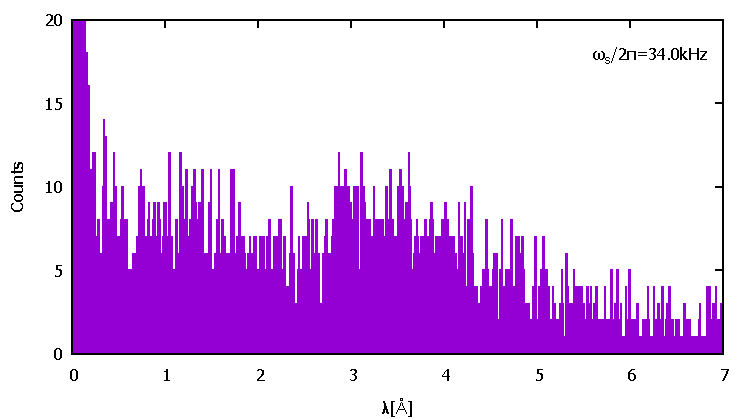
\includegraphics[height=4.3cm]{resonance/results/Flipper1_RawCounts_340kHz.pdf}
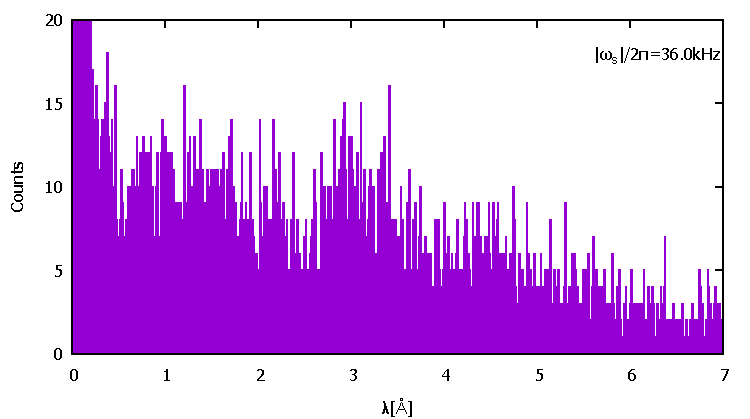
\includegraphics[height=4.3cm]{resonance/results/Flipper1_RawCounts_360kHz.pdf}\\
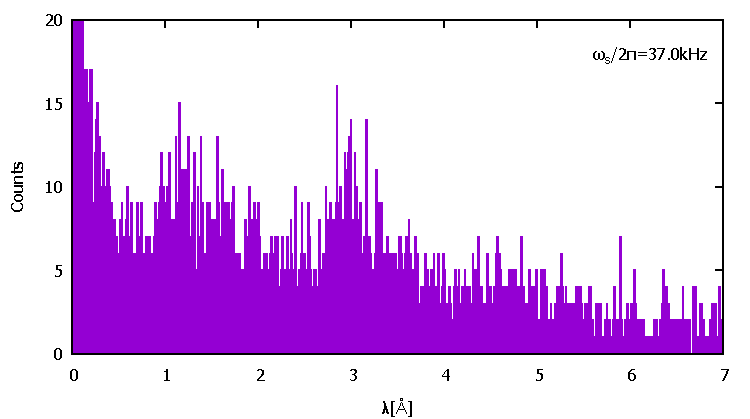
\includegraphics[height=4.3cm]{resonance/results/Flipper1_RawCounts_370kHz.pdf}
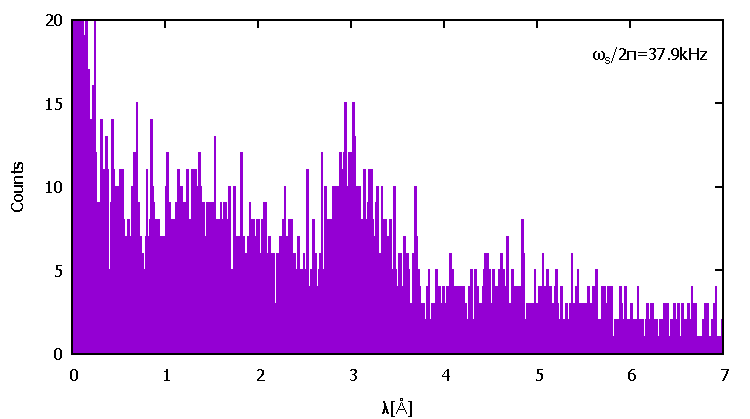
\includegraphics[height=4.3cm]{resonance/results/Flipper1_RawCounts_379kHz.pdf}\\
%\end{minipage}
%\begin{minipage}{0.49\hsize}
%\centering
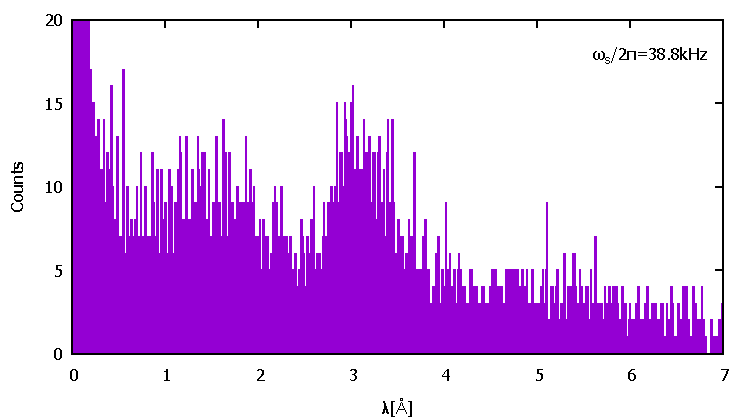
\includegraphics[height=4.3cm]{resonance/results/Flipper1_RawCounts_388kHz.pdf}
\includegraphics[height=4.3cm]{resonance/results/Flipper1_RawCounts_400kHz.pdf}\\
\includegraphics[height=4.3cm]{resonance/results/Flipper1_RawCounts_410kHz.pdf}
%\vspace{4.3cm}
%\end{minipage}
\caption{上流フリッパー共鳴実験で得られた粒子数の波長分布}\label{Resonance_fig_Flipper1_RawCounts}
\end{figure}

\begin{figure}[h]
%\begin{minipage}{0.5\hsize}
%\centering
\includegraphics[height=4.3cm]{resonance/results/Flipper2_RawCounts_-20A.pdf}
\includegraphics[height=4.3cm]{resonance/results/Flipper2_RawCounts_-10A.pdf}\\
\includegraphics[height=4.3cm]{resonance/results/Flipper2_RawCounts_-5A.pdf}
\includegraphics[height=4.3cm]{resonance/results/Flipper2_RawCounts_0A.pdf}\\
\includegraphics[height=4.3cm]{resonance/results/Flipper2_RawCounts_1A.pdf}
%\end{minipage}
%\begin{minipage}{0.5\hsize}
%\centering
\includegraphics[height=4.3cm]{resonance/results/Flipper2_RawCounts_3A.pdf}\\
\includegraphics[height=4.3cm]{resonance/results/Flipper2_RawCounts_5A.pdf}
\includegraphics[height=4.3cm]{resonance/results/Flipper2_RawCounts_10A.pdf}\\
\includegraphics[height=4.3cm]{resonance/results/Flipper2_RawCounts_20A.pdf}
%\vspace{4.3cm}
%\end{minipage}
\caption{下流フリッパー共鳴実験で得られた粒子数の波長分布}\label{Resonance_fig_Flipper2_RawCounts}
\end{figure}

\clearpage
\subsection{分析}
以下では
\begin{enumerate}
\item 上流フリッパーについてデータから共鳴条件(\ref{Resonance_resonance})を満たす$\omega_s$を決め、グラフから共鳴時に最もよくスピン反転する中性子の波長を推定し、$\pi$フリップ条件(\ref{Resonance_piflip})から$\omega_r$を計算する。
\item 上流フリッパーについてデータから共鳴条件(\ref{Resonance_resonance})を満たす$I_c$を決め、グラフから共鳴時に最もよくスピン反転する中性子の波長を推定し、$\pi$フリップ条件(\ref{Resonance_piflip})から$\omega_r$を計算する。
\end{enumerate}
という流れでデータの分析を行う。

\paragraph{上流フリッパーに関する分析}
共鳴しているかを知るにはパラメータを変えたときの検出粒子数を比較すればよく、ある波長でカウントが最小となるとき共鳴していると考えてよい。しかし前節で示したデータは測定時間や加速器の出力がそれぞれ異なるので、そのままでは互いに比較することができない。そこで測定データのカウントをそのデータの測定開始時刻から測定終了時刻までにおけるLiMのカウントで割って規格化することで、データを互いに比較できるようにする。このようにして規格化した上流フリッパー共鳴実験における粒子数の波長分布を、フリッパーをOFFにしたときの規格化粒子数と共に、図\ref{Resonance_fig_Flipper1_NormalizedCounts}に表す。

\begin{figure}[h]
%\begin{minipage}{0.49\hsize}
%\centering
\includegraphics[height=4.3cm]{resonance/analysis/Flipper1_NormalizedCounts_340kHz.pdf}
\includegraphics[height=4.3cm]{resonance/analysis/Flipper1_NormalizedCounts_360kHz.pdf}\\
\includegraphics[height=4.3cm]{resonance/analysis/Flipper1_NormalizedCounts_370kHz.pdf}
\includegraphics[height=4.3cm]{resonance/analysis/Flipper1_NormalizedCounts_379kHz.pdf}\\
%\end{minipage}
%\begin{minipage}{0.49\hsize}
%\centering
\includegraphics[height=4.3cm]{resonance/analysis/Flipper1_NormalizedCounts_388kHz.pdf}
\includegraphics[height=4.3cm]{resonance/analysis/Flipper1_NormalizedCounts_400kHz.pdf}\\
\includegraphics[height=4.3cm]{resonance/analysis/Flipper1_NormalizedCounts_410kHz.pdf}
%\vspace{4.3cm}
%\end{minipage}
\caption{上流フリッパー共鳴実験における規格化粒子数の波長分布}\label{Resonance_fig_Flipper1_NormalizedCounts}
\end{figure}

さらに、図\ref{Resonance_fig_Flipper1_CountsRate}にフリッパーONのときの規格化粒子数をフリッパーOFFのときの規格化粒子数で割ったもの、すなわち上流フリッパーでスピン反転しなかった割合の波長分布を表す。図\ref{Resonance_fig_Flipper1_CountsRate}を見ると、波長$\lambda=$3.0{\AA}から4.5{\AA}あたりで大きく凹んでいることがわかる。
\begin{figure}[h]
%\begin{minipage}{0.49\hsize}
%\centering
\includegraphics[height=4.3cm]{resonance/analysis/Flipper1_CountsRate_340kHz.pdf}
\includegraphics[height=4.3cm]{resonance/analysis/Flipper1_CountsRate_360kHz.pdf}\\
\includegraphics[height=4.3cm]{resonance/analysis/Flipper1_CountsRate_370kHz.pdf}
\includegraphics[height=4.3cm]{resonance/analysis/Flipper1_CountsRate_379kHz.pdf}\\
%\end{minipage}
%\begin{minipage}{0.49\hsize}
%\centering
\includegraphics[height=4.3cm]{resonance/analysis/Flipper1_CountsRate_388kHz.pdf}
\includegraphics[height=4.3cm]{resonance/analysis/Flipper1_CountsRate_400kHz.pdf}\\
\includegraphics[height=4.3cm]{resonance/analysis/Flipper1_CountsRate_410kHz.pdf}
%\vspace{4.3cm}
%\end{minipage}
\caption{上流フリッパーにおいてスピン反転しなかった割合}\label{Resonance_fig_Flipper1_CountsRate}
\end{figure}

そこで、図\ref{Resonance_fig_Flipper1_NormalizedCounts}の波長領域$\lambda=$3.0{\AA}から4.5{\AA}における規格化粒子数の和を$|\omega_s|/2\pi$を横軸に取って図示すると図\ref{Resonance_fig_Flipper1_Freq}のようになる。2次関数でフィッティングした結果、最もカウントが少なくなる、すなわち共鳴条件(\ref{Resonance_resonance})を満たす$\omega_s$として$|\omega_s|/2\pi=37.17\pm0.03$kHzと決まった。
\begin{comment}
\begin{table}[h]
\centering
\begin{tabular}{c|lllllll}
$|\omega_s|/2\pi$&34.0&36.0&37.0&37.9&38.8&40.0&41.0\\
$3.0{\AA}-4.5{\AA}での規格化粒子数($\times 10^{-4}$)&$17.8\pm0.8$&18.4\pm
\end{comment}
\begin{figure}[h]
\centering
\includegraphics[width=12cm]{resonance/analysis/Flipper1_Freq_30-45r.pdf}
\caption{$|\omega_s|/2\pi$に対する波長$\lambda=$3.0{\AA}から4.5{\AA}における規格化粒子数}\label{Resonance_fig_Flipper1_Freq}
\end{figure}

次に、決まった$\omega_s$と最も近い$|\omega_s|/2\pi=37.0$kHzのときのスピン反転しなかった割合の波長分布(図\ref{Resonance_fig_Flipper1_CountsRate_370fit})から、最も反転しない割合が低い、すなわち最も反転する波長を推定すると、2次関数フィットの結果、$\lambda=3.66\pm0.05${\AA}と求まった。これを速度に直すと$v=1080\pm15$m/sとなり、この速度が$\pi$フリップ条件(\ref{Resonance_piflip})を満たすことから$\omega_{r1}/2\pi=9.0\pm0.1$kHzと計算される。
\begin{figure}[h]
\centering
\includegraphics[width=12cm]{resonance/analysis/Flipper1_CountsRate_370kHz_fit.pdf}
\caption{$|\omega_s|/2\pi$=37.0kHzのときのスピン反転しなかった割合の波長分布}\label{Resonance_fig_Flipper1_CountsRate_370fit}
\end{figure}

\paragraph{下流フリッパーに関する分析}
上流フリッパー同様に下流フリッパーの測定データについても互いに比較するために、測定時間のLiMカウントで規格化を行う。その結果を図\ref{Resonance_fig_Flipper2_NormalizedCounts}に表す。
\begin{figure}[h]
%\begin{minipage}{0.49\hsize}
%\centering
\includegraphics[height=4.3cm]{resonance/analysis/Flipper2_NormalizedCounts_-20A.pdf}
\includegraphics[height=4.3cm]{resonance/analysis/Flipper2_NormalizedCounts_-10A.pdf}\\
\includegraphics[height=4.3cm]{resonance/analysis/Flipper2_NormalizedCounts_-5A.pdf}
\includegraphics[height=4.3cm]{resonance/analysis/Flipper2_NormalizedCounts_0A.pdf}\\
%\end{minipage}
%\begin{minipage}{0.49\hsize}
%\centering
\includegraphics[height=4.3cm]{resonance/analysis/Flipper2_NormalizedCounts_1A.pdf}
\includegraphics[height=4.3cm]{resonance/analysis/Flipper2_NormalizedCounts_3A.pdf}\\
\includegraphics[height=4.3cm]{resonance/analysis/Flipper2_NormalizedCounts_5A.pdf}
\includegraphics[height=4.3cm]{resonance/analysis/Flipper2_NormalizedCounts_10A.pdf}\\
%\vspace{4.3cm}
%\end{minipage}
\includegraphics[height=4.3cm]{resonance/analysis/Flipper2_NormalizedCounts_20A.pdf}
\caption{下流フリッパー共鳴実験における規格化粒子数の波長分布}\label{Resonance_fig_Flipper2_NormalizedCounts}
\end{figure}

さらに、図\ref{Resonance_fig_Flipper2_CountsRate}にフリッパーONのときの規格化粒子数をフリッパーOFFのときの規格化粒子数で割ったもの、すなわち上流フリッパーでスピン反転しなかった割合の波長分布を表す。図\ref{Resonance_fig_Flipper2_CountsRate}を見ると、波長$\lambda=$3.0{\AA}から4.0{\AA}あたりで大きく凹んでいることがわかる。
\begin{figure}[h]
%\begin{minipage}{0.49\hsize}
%\centering
\includegraphics[height=4.3cm]{resonance/analysis/Flipper2_CountsRate_-20A.pdf}
\includegraphics[height=4.3cm]{resonance/analysis/Flipper2_CountsRate_-10A.pdf}\\
\includegraphics[height=4.3cm]{resonance/analysis/Flipper2_CountsRate_-5A.pdf}
\includegraphics[height=4.3cm]{resonance/analysis/Flipper2_CountsRate_0A.pdf}\\
%\end{minipage}
%\begin{minipage}{0.49\hsize}
%\centering
\includegraphics[height=4.3cm]{resonance/analysis/Flipper2_CountsRate_1A.pdf}
\includegraphics[height=4.3cm]{resonance/analysis/Flipper2_CountsRate_3A.pdf}\\
\includegraphics[height=4.3cm]{resonance/analysis/Flipper2_CountsRate_5A.pdf}
\includegraphics[height=4.3cm]{resonance/analysis/Flipper2_CountsRate_10A.pdf}\\
%\vspace{4.3cm}
%\end{minipage}
\includegraphics[height=4.3cm]{resonance/analysis/Flipper2_CountsRate_20A.pdf}
\caption{下流フリッパーにおいてスピン反転しなかった割合}\label{Resonance_fig_Flipper2_CountsRate}
\end{figure}

そこで、図\ref{Resonance_fig_Flipper2_NormalizedCounts}の波長領域$\lambda=$2.7{\AA}から4.2{\AA}における規格化粒子数を数え、$I_c$を横軸として図示すると図\ref{Resonance_fig_Flipper2_Cur}のようになる。2次関数でフィッティングした結果、最もカウントが少なくなる、すなわち共鳴条件(\ref{Resonance_resonance})を満たす$I_c$として$I_c=0.7\pm0.1$Aと決まった。
\begin{figure}[h]
\centering
\includegraphics[width=12cm]{resonance/analysis/Flipper2_Cur_30-40.pdf}
\caption{$I_c$に対する波長$\lambda=$3.0{\AA}から4.0{\AA}における規格化粒子数}\label{Resonance_fig_Flipper2_Cur}
\end{figure}

次に、決まった$I_c$の中心値と最も近い$I_c=0.7$Aのときのスピン反転しなかった割合の波長分布(図\ref{Resonance_fig_Flipper2_CountsRate_7fit})から、最も反転しない割合が低い、すなわち最も反転する波長を推定すると、2次関数フィットの結果、$\lambda=3.40\pm0.03${\AA}と求まった。これを速度に直すと$v=1163\pm10$m/sとなり、この速度が$\pi$フリップ条件(\ref{Resonance_piflip})を満たすことから$\omega_{r2}/2\pi=9.6\pm0.1$kHzと計算される。
\begin{figure}[h]
\centering
\includegraphics[width=12cm]{resonance/analysis/Flipper2_CountsRate_7A_fit.pdf}
\caption{$I_c$=0.7Aのときのスピン反転しなかった割合の波長分布}\label{Resonance_fig_Flipper2_CountsRate_7fit}
\end{figure}

\clearpage
\paragraph{分析まとめ}
以上の分析から各パラメータは次のように決まった。
\begin{table}[h]
\centering
\begin{tabular}{|c|c|} \hline
$|\omega_s|/2\pi$&$37.17\pm0.03$kHz\\ \hline
$I_c$&$0.7\pm0.1$A \\ \hline
$\omega_{r1}/2\pi$&$9.0\pm0.1$kHz \\ \hline
$\omega_{r2}/2\pi$&$9.6\pm0.1$kHz \\ \hline
\end{tabular}
\end{table}

しかし、実験中の粗い解析では$|\omega_s|/2\pi=37.5\pm0.1$kHz,$I_c=0.185\pm0.11$Aと求まったため、実際には以後、
\begin{table}[h]
\centering
\begin{tabular}{|c|c|} \hline
$|\omega_s|/2\pi$&37.5kHz\\ \hline
$I_c$&0.185A \\ \hline
\end{tabular}
\end{table}

\noindent として実験を進めた。このことによる共鳴条件からのずれは最大で$\epsilon/|\omega_z|=$0.1程度であり、十分小さいといえる(図\ref{Resonance_fig_visivility},\ref{Resonance_fig_interference}参照)。

\begingroup
\def\imgwidth{5.5cm}

\section{位相シフタコイルによる干渉}
本実験である位相シフタコイルによる干渉について、実験手順、結果、解析の順に説明する。

\subsection{実験手順}
位相シフタコイルに流す電流を、0.0Aから3.3A, -0.3から-1.5までそれぞれ0.3A刻みで変え、各点10分程度測定した。

\subsection{実験結果}
干渉を見るためには、中性子のTOF(波長)を制限する必要がある。
どの波長を選ぶべきか判断するために、様々な波長での実験か結果をフィットして、最もビジビリティが高かった波長を採用することにする。

\paragraph{ビジビリティが最高となる波長}
上流フリッパーと下流フリッパーの反転率が1/2となるのは、予備実験からそれぞれ3.75Å, 3.56Åである。
その付近のいくつかの波長領域について、横軸を位相シフタに流した電流、縦軸をカウント数/LiMのカウント数で割ったものとしてプロットする。
実線は$-A\cos(Bx+C)+D$でフィットした結果を示している。
\begin{figure}[H]
\centering
\begin{minipage}{0.33\hsize}
\includegraphics[width=\imgwidth]{phase_shifter/wl/wlf1.pdf}
\end{minipage}
\begin{minipage}{0.33\hsize}
\includegraphics[width=\imgwidth]{phase_shifter/wl/wlf2.pdf}
\end{minipage}
\begin{minipage}{0.33\hsize}
\includegraphics[width=\imgwidth]{phase_shifter/wl/wlf3.pdf}
\end{minipage}\\
\begin{minipage}{0.33\hsize}
\includegraphics[width=\imgwidth]{phase_shifter/wl/wlf12.pdf}
\end{minipage}
\begin{minipage}{0.33\hsize}
\includegraphics[width=\imgwidth]{phase_shifter/wl/wlf4.pdf}
\end{minipage}
\begin{minipage}{0.33\hsize}
\includegraphics[width=\imgwidth]{phase_shifter/wl/wlf5.pdf}
\end{minipage}
\begin{minipage}{0.33\hsize}
\includegraphics[width=\imgwidth]{phase_shifter/wl/wlf11.pdf}
\end{minipage}
\begin{minipage}{0.33\hsize}
\includegraphics[width=\imgwidth]{phase_shifter/wl/wlf6.pdf}
\end{minipage}
\begin{minipage}{0.33\hsize}
\includegraphics[width=\imgwidth]{phase_shifter/wl/wlf7.pdf}
\end{minipage}
\begin{minipage}{0.33\hsize}
\includegraphics[width=\imgwidth]{phase_shifter/wl/wlf9.pdf}
\end{minipage}
\begin{minipage}{0.33\hsize}
\includegraphics[width=\imgwidth]{phase_shifter/wl/wlf10.pdf}
\end{minipage}
\begin{minipage}{0.33\hsize}
\includegraphics[width=\imgwidth]{phase_shifter/wl/wlf8.pdf}
\end{minipage}
\caption{各波長領域におけるカウント数/LiMカウント数。横軸は位相シフタコイルに流した電流。}
\end{figure}

フィット結果からビジビリティ$V\equiv A/D$を算出し、プロットすると以下のようになる:
\begin{figure}[H]
\centering
\includegraphics{phase_shifter/visibility.pdf}
\caption{波長ごとのビジビリティ。誤差はフィッティング誤差に由来する。}
\end{figure}

$\lambda=3.42\pm0.07$Åで最もビジビリティが高くなっていることがわかる。

\paragraph{最高ビジビリティとなる波長における結果}
$\lambda=3.42\pm0.07$Åにおける実験結果を以下に示す。
今後の解析はこの波長で行うことにする。
\begin{figure}[H]
\centering
\includegraphics{phase_shifter/fit.pdf}
\caption{$\lambda=3.42\pm0.07$Åにおける実験結果とフィット。\label{ps_fitresult}}
\end{figure}

\subsection{解析}
\paragraph{理論値との対応}
図\ref{ps_fitresult}の縦軸はカウント数/LiMカウント数であり、これは理論値と直接対応する値ではない。
これを理論値と対応付けるために、$|\langle\uparrow|\uparrow\rangle|^2$に対応する、フリッパーをオフにしてスピンをフリップさせずに検出
した時のカウント数/LiMカウント数で割る必要がある。

$\lambda=3.42\pm0.07$Åにおける$|\langle\uparrow|\uparrow\rangle|^2$に対応するカウント数/LiMカウント数は、
$(6.73\pm0.53)\times10^{-4}$であった。この値で規格化した実験結果とフィット結果は以下の通りである:
\begin{figure}[H]
\centering
\includegraphics{phase_shifter/highest.pdf}
\end{figure}
\begin{table}[H]
\centering
\begin{tabular}{|r|r|}
\hline
$A$&$0.28\pm0.03$\\
\hline
$B$&$4.42\pm$0.04\\
\hline
$C$&$2.04\pm0.06$\\
\hline
$D$&$0.585\pm0.04$\\
\hline
\end{tabular}
\caption{フィット結果。フィット関数は$-A\cos(Bx+C)+D$}
\end{table}

\paragraph{理論値との比較}
理論式(\ref{theoretical})との比較を行う。
理論式
\begin{align}
|({\psi}_{Ⅶ}(x,t))_{+}|^2
=1-\cos^2\left({\omega}d'/v\right)\sin^2\left(\frac{2\omega_{r}}{v}d\right)\tag{\ref{theoretical}}
\end{align}
のうち、$\sin^2(2\omega_{r}/vd)$については、今$\pi/2$フリップ条件を満たしていることを仮定すれば1である。
従って、以下のように簡略化することができる:
\begin{align}
|({\psi}_{Ⅶ}(x,t))_{+}|^2=\frac{1}{2}\left(
1-\cos\frac{2{\omega}d'}{v}
\right)
\end{align}

$\omega$を電流に対応させることで、理論式の$B$は$4.34$となる。
以上より、理論式のパラメーターをまとめると以下のようになる:
\begin{table}[H]
\centering
\begin{tabular}{|r|r|}
\hline
$A$&$0.5$\\
\hline
$B$&$4.34$\\
\hline
$C$&$0$\\
\hline
$D$&$0.5$\\
\hline
\end{tabular}
\caption{フィット結果。フィット関数は$-A\cos(Bx+C)+D$}
\end{table}

角振動数$B$については$2\sigma$の精度で一致していることがわかる。振幅$A$、位相$C$、オフセット$D$にはずれが見られる。
すれの原因については、後により深く考察する。

\endgroup
\section{解析}
実験で得られたデータからははっきりと波うつパターンが見て取れる。この章ではその波模様をいくつかの要素に分解し、それぞれについて理論的に説明できるかどうかを考えてゆく。私たちは望んだ干渉の結果を見ることができたのか。

\subsection{波の分解}

\ref{Resonance_sec}章で述べたように、干渉パターンは最も一般的には、共鳴からのずれを表すパラメータ$\epsilon$と中性子の速度$v$に依存した係数$N_1,N_2,N_3$を用いて
\begin{equation}
I=N_1-N_2\cos\left(\frac{2}{v}(\omega d'-\epsilon L')\right) -N_3\sin\left(\frac{2}{v}(\omega d'-\epsilon L')\right) \label{analysis_theory_ippan}
\end{equation}
と表せる。ここで$\omega$は位相シフタコイルの磁場$B_p$を用いて$\omega=|\mu_n|B_p$と表される量であり、$d',L'$はそれぞれ位相シフタコイルの幅、2つのスピンフリッパー間距離である。さらに$N_4=\sqrt{N_2^2+N_3^2}$として
\begin{equation}
\cos \phi=\frac{N_2}{N_4}, \quad \sin \phi=\frac{N_3}{N_4}
\end{equation}
で$\phi$を定義すれば、干渉パターンは
\begin{equation}
I=N_1-N_4\cos\left(\frac{2}{v}(\omega d'-\epsilon L')-\phi\right)\label{analysis_theory_ippan2}
\end{equation}
と書き直される。このように書くと実験データをフィッティングして得られる4つのパラメータと理論式を対応づけることができる。すなわち、実験で得られた波模様を位相シフタコイルに流した電流$I_p$に対して
\begin{equation}
I=D-A\cos(B\cdot I_p+C)
\end{equation}
という関数でフィッティングしたときの4つのパラメータ$A,B,C,D$は理論と
\begin{comment}
\renewcommand{\arraystretch}{1.5}
\begin{equation}
\begin{array}{l}
A \leftrightarrow N_4\\
B \leftrightarrow \dfrac{2\omega d'}{v(-I_p)}\\
C \leftrightarrow \dfrac{2\epsilon L'}{v} +\phi \\
D \leftrightarrow N_1
\end{array}
\end{equation}
\renewcommand{\arraystretch}{1}
\end{comment}
\begin{align}
A \leftrightarrow N_4&&B \leftrightarrow \dfrac{2\omega d'}{v(-I_p)}&&C \leftrightarrow \dfrac{2\epsilon L'}{v} +\phi&&D \leftrightarrow N_1
\end{align}
と対応づくことがわかる。なお、$I_p$は鉛直下向きに磁場が発生する向きを正としたため、$B,C$については理論式(\ref{analysis_theory_ippan})のコサインの中身にマイナスをかけて対応づけておく。

なお、実験で得られたデータはある波長領域について積分したものであるため、ひとつの波長に対して定められた理論式(\ref{analysis_theory_ippan})とは厳密には対応づかない。しかし十分狭い波長領域で見れば、近似的に領域の中心の波長に対する理論式とその波長領域での実験値を対応づけることができる。このことの詳しい議論は後で行う。

ここで行ったことの要は、単に実験と理論を対応づけたということではなく、波模様というあいまいな概念を輪郭の明確な4つの要素に分解したことにある。これによって私たちは奇妙にゆれる波に惑わされることなく、個々の要素について着実に考えてゆくことができる。

\subsection{$B$}
\paragraph{パラメータ$B$の意味}
$B$には干渉という現象のエッセンスが凝縮されている。上では干渉パターンの最も一般的な形を見たが、逆に最も特殊な場合を見てみよう。それは共鳴条件()が満たされている中で、$\pi/2$フリップ条件()を満たす速度の中性子を対象とした場合である。そのときは$N_1=1/2,N_2=1/2,N_3=0,\epsilon=0$であるから、干渉パターンは
\begin{equation}
I=\frac{1}{2}\left(1-\cos\frac{2\omega d'}{v}\right) \label{analysis_theory_simple}
\end{equation}
となる。このように、非常にシンプルな場合を考えてもスピン上下の位相差を表す$B$の部分の形は変わらない。そのような意味で$B$は干渉の本質を担っている。

\paragraph{理論からのアプローチ}
理論的には$B$は$2\omega d'/v(-I_p)$と書かれるが、$\omega \propto -I_p$であって、具体的に書けば
\begin{align}
\omega d'=\frac{|\mu_n|B_p d'}{\hbar}=\frac{(-I_p)|\mu_n| b_p d'}{\hbar}
\end{align}
となる。ここで$b_p$は位相シフタコイルに1Aの電流を流したときに発生する磁束密度。なおこの章では実験値と理論値を比較する必要からSI単位系を用い、$\hbar$も明記する。さらに位相シフタコイルによる磁場は空間的に一様ではないため、実際は粒子の軌道に沿った積分で表す必要がある:
\begin{equation}
b_p d' \rightarrow \int b_p(x) dx
\end{equation}

次の図\ref{analysis_fig_PhaseShifterSimulation}は位相シフタコイルに1Aの電流を流したときの磁場分布シミュレーション結果である。%またシフタコイルの中心($y=z=0$)を通ったときの$x$軸に沿っての磁場分布を図\ref{analysis_fig_PSS_danmen}に表す。
このシミュレーションを用いて$\int b_p(x) dx$を計算すると、シフタコイルの中心($y=z=0$)を通ったときの積分値は
\begin{equation}
\int b_p(x) dx =2.75 \times 10^{-5} \mathrm{T\cdot m/A}
\end{equation}
となった。なお積分範囲は実際の配置と図\ref{analysis_fig_PSS_danmen}より、$-20$cmから$20$cmとした。また粒子の経路が$y$方向や$z$方向にずれたときの積分値は図\ref{analysis_fig_PSS_zure}のようになった。ビームの幅は20mm程度であるから、中性子の経路による積分値のずれは1\%程度に抑えられると考えられる。そこで今後の解析には中心での値を用いることにする。
\begin{figure}[h]
\centering
\includegraphics[width=9cm]{analysis/B/bd.pdf}
\caption{$y,z$方向のずれによる影響} \label{analysis_fig_PSS_zure}
\vspace{-5mm}
\end{figure}

ゆえに$B$の理論値は
\begin{equation}
\frac{2\omega d'}{v(-I_p)}=2\frac{|\mu_n|\int b_p dx}{\hbar v}=2\frac{|\mu_n|\int b_p dx}{\hbar}\frac{m}{h}\lambda=1.27 \cdot \lambda \ [1/A] \label{analysis_theory_B}
\end{equation}
となる。ただし$\lambda$[\AA]は中性子の波長。 

\begin{figure}[H]
%\begin{minipage}{0.5\hsize}
\begin{center}
\includegraphics[width=9cm]{analysis/B/coil11_image1.pdf}
\vspace{-1mm}
\subcaption{横から}
\vspace{-3mm}
%\end{minipage}
%\begin{minipage}{0.5\hsize}
%\centering
\includegraphics[width=9cm]{analysis/B/coil11_image2.pdf}
\vspace{-1mm}
\subcaption{上から}
\vspace{-3mm}
%\end{minipage}\\
%\begin{center}
\includegraphics[width=9cm]{analysis/B/coil11_danmen1.pdf}
\vspace{-1mm}
\subcaption{中心($y=z=0$)を通ったとき}
\vspace{-3mm}
\end{center}
%\end{center}
\caption{位相シフタコイル磁場分布シミュレーション} \label{analysis_fig_PhaseShifterSimulation}
%\vspace{-1cm}
\end{figure}

\paragraph{実験結果・解析}
以下の表\ref{analysis_tbl_B}に波長領域$\lambda \pm 0.07 \AA$における実験データから得られた$B$の値と式(\ref{analysis_theory_B})から得られる理論値を示す。なお理論値には中性子の経路による誤差1\% が含まれるとした。また表\ref{analysis_tbl_B}の結果を図\ref{analysis_fig_B}に表す。図、表からわかるように全ての波長領域でパラメータ$B$の実験値と理論値はよく一致しており、多くの波長において誤差の範囲で一致している。

\begin{figure}[h]
\begin{minipage}{0.35\hsize}
\centering
\makeatletter
\def\@captype{table}
\makeatother
\caption{各波長領域におけるパラメータ$B$の実験値と理論値} \label{analysis_tbl_B}
\begin{tabular}{lll}
$\lambda$[\AA] &  $B(実験)$ &   理論値 \\ \hline
3.06  & 4.18  $\pm$ 0.05  & 3.90  $\pm$ 0.04  \\
3.21  & 4.14  $\pm$ 0.05  & 4.08  $\pm$ 0.04  \\
3.35  & 4.32  $\pm$ 0.05  & 4.27  $\pm$ 0.04  \\
3.42  & 4.42  $\pm$ 0.04  & 4.36  $\pm$ 0.04  \\
3.50  & 4.52  $\pm$ 0.05  & 4.45  $\pm$ 0.04  \\
3.56  & 4.63  $\pm$ 0.07  & 4.54  $\pm$ 0.05  \\
3.66  & 4.74  $\pm$ 0.07  & 4.66  $\pm$ 0.05  \\
3.75  & 4.77  $\pm$ 0.09  & 4.78  $\pm$ 0.05  \\
3.86  & 5.09  $\pm$ 0.09  & 4.91  $\pm$ 0.05  \\
4.00  & 5.15  $\pm$ 0.08  & 5.10  $\pm$ 0.05  \\
4.15  & 5.16  $\pm$ 0.18  & 5.28  $\pm$ 0.05  \\
4.29  & 3.36  $\pm$ 0.17  & 5.47  $\pm$ 0.05  \\ \hline
\end{tabular}
\end{minipage}
\begin{minipage}{0.65\hsize}
\centering
\vspace{2.5cm}
\includegraphics[width=10cm]{analysis/B/B_F.pdf}
\caption{各波長領域に対する$B$} \label{analysis_fig_B}
\end{minipage}
\end{figure}

\paragraph{結論}
パラメータ$B$こそスピン干渉の本質であり、それが干渉のみられた全ての波長領域で理論値とよく一致したということは、私たちが望みのものを手に入れたということを示唆している。目的は果たされた。

\subsection{$C$}
\paragraph{パラメータ$C$の意味}
干渉においてパラメータ$B$の次に重要な意味をもつパラメータは$C$であろう。最もシンプルな場合(\ref{analysis_theory_simple})を考えると、理論的にはパラメータ$C$に対応する位相のシフトは入ってこなかった:
\begin{equation}
I=\frac{1}{2}\left(1-\cos\frac{2\omega d'}{v}\right)
\end{equation}
$C$の対応物$2\epsilon L'/v +\phi$は、どちらの項も$\epsilon=0$のときゼロとなるためである。すなわちパラメータ$C$は共鳴からのずれに依存する。パラメータ$C$を分析することで、共鳴からのずれを知ることができる。

\paragraph{理論からのアプローチ}
理論的には$C$は$2\epsilon L'/v +\phi$に対応し、$\cos\phi=N_2/N_4,\sin\phi=N_3/N_4$であった。\ref{Resonance_sec}章より
\begin{align}
&N_2 = 2\left(\frac{\omega_r}{\omega_A}\right)^2\sin^2\frac{\omega_A}{v}d \left(\cos^2 \frac{\omega_A}{v}d -\left(\frac{\epsilon}{\omega_A}\right)^2 \sin^2 \frac{\omega_A}{v}d\right) \\
&N_3 = 4\frac{\epsilon}{\omega_A} \left(\frac{\omega_r}{\omega_A}\right)^2\sin^3\frac{\omega_A}{v}d \cos \frac{\omega_A}{v}d
\end{align}
であるから$N_4$は
\begin{equation}
N_4=\sqrt{N_2^2+N_3^2}=2\left(\frac{\omega_r}{\omega_A}\right)^2\sin^2\frac{\omega_A}{v}d \left(\cos^2\frac{\omega_A}{v}d+\left(\frac{\epsilon}{\omega_A}\right)^2\sin^2\frac{\omega_A}{v}d\right)
\end{equation}
と書ける。ここで$\omega_A=\sqrt{\epsilon^2+\omega_r^2}$であり、$d$はフリッパーの幅である。よって
\begin{align}
\cos\phi&=\frac{\cos^2 \frac{\omega_A}{v}d -\left(\frac{\epsilon}{\omega_A}\right)^2 \sin^2 \frac{\omega_A}{v}d}{\cos^2\frac{\omega_A}{v}d+\left(\frac{\epsilon}{\omega_A}\right)^2\sin^2\frac{\omega_A}{v}d} \\
\sin\phi&=\frac{2\frac{\epsilon}{\omega_A}\sin\frac{\omega_A}{v}d \cos \frac{\omega_A}{v}d}{\cos^2\frac{\omega_A}{v}d+\left(\frac{\epsilon}{\omega_A}\right)^2\sin^2\frac{\omega_A}{v}d}
\end{align}
であり、確かに$\epsilon=0$のとき$\phi=0$となる。次の図\ref{analysis_fig_phi}に$\epsilon/\omega_z=0,0.1,0.3,0.5,1.0$のときの中性子の波長$\lambda$に対する$\phi$の理論値を表す。ただし$\omega_r/\omega_z=0.25,B_z=12.8\,\mathrm{G}$とした。
\begin{figure}[h]
\centering
\includegraphics[width=10cm]{analysis/C/chi.pdf}
\caption{中性子の波長$\lambda$に対する$\phi$} \label{analysis_fig_phi}
\end{figure}

これを実験値と比べるためにはもう一工夫必要となる。理論では上流と下流のスピンフリッパーで$\omega_r$の値は等しいとしていた。しかし、実際に測定データから得られた$\omega_r$は上流と下流で異なっていた(\ref{Resonance_sec}章参照)。%上流、下流フリッパーの$\omega_r$をそれぞれ$\omega_{r1},\omega_{r2}$とすると$\omega_r/2\pi=8.7\pm0.1\,\mathrm{kHz},
そこで上流、下流フリッパーの$\omega_r$をそれぞれ$\omega_{r1},\omega_{r2}$として、2つのフリッパーで$\omega_r$が異なる場合も含めた干渉パターンの式を求めると、式の形は$\omega_r$が等しい場合(\ref{analysis_theory_ippan})と同じで、係数が
\begin{align}
&N_1 = \left(\cos^2 \frac{\omega_{A1}}{v}d +\left(\frac{\epsilon}{\omega_{A1}}\right)^2\sin^2 \frac{\omega_{A1}}{v}d\right)\left(\cos^2 \frac{\omega_{A2}}{v}d+\left(\frac{\epsilon}{\omega_{A2}}\right)^2 \sin^2 \frac{\omega_{A2}}{v}d\right)\\ \notag
&\hspace{7cm}+\left(\frac{\omega_{r1}}{\omega_{A1}}\right)^2\left(\frac{\omega_{r2}}{\omega_{A2}}\right)^2 \sin^2 \frac{\omega_{A1}}{v}d \sin^2 \frac{\omega_{A2}}{v}d\\
&N_2 = 2\frac{\omega_{r1}}{\omega_{A1}}\frac{\omega_{r2}}{\omega_{A2}}\sin\frac{\omega_{A1}}{v}d\sin\frac{\omega_{A2}}{v}d \left(\cos \frac{\omega_{A1}}{v}d\cos \frac{\omega_{A2}}{v}d -\frac{\epsilon}{\omega_{A1}}\frac{\epsilon}{\omega_{A2}} \sin \frac{\omega_{A1}}{v}d\sin \frac{\omega_{A2}}{v}d\right) \\
&N_3 = 2\frac{\omega_{r1}}{\omega_{A1}}\frac{\omega_{r2}}{\omega_{A2}}\sin\frac{\omega_{A1}}{v}d\sin\frac{\omega_{A2}}{v}d \left(\frac{\epsilon}{\omega_{A1}}\sin \frac{\omega_{A1}}{v}d\cos \frac{\omega_{A2}}{v}d +\frac{\epsilon}{\omega_{A2}} \sin \frac{\omega_{A1}}{v}d\cos \frac{\omega_{A2}}{v}d\right)
\end{align}\label{analysis_theory_ippanippan}
となる。ここで$\omega_{Ai}=\sqrt{\epsilon^2+\omega_{ri}^2} \ (i=1,2)$である。これでパラメータ$C$について実験値と理論値を比較する準備が整った。

\paragraph{実験結果}
以下の表\ref{analysis_tbl_C}に波長領域$\lambda \pm 0.07 \AA$における実験データから得られた$C$の値を示し、中心波長$\lambda$と$C$の関係を図\ref{analysis_fig_C}に表す。
\begin{figure}[h]
\begin{minipage}{0.35\hsize}
\centering
\makeatletter
\def\@captype{table}
\makeatother
\caption{各波長領域におけるパラメータ$C$の実験値} \label{analysis_tbl_C}
\begin{tabular}{ll}
$\lambda$[\AA] &  $C(実験)$\\ \hline
3.06 	&	1.12 	$\pm$	0.09 \\
3.21 	&	1.61 	$\pm$	0.09 \\
3.35 	&	1.90 	$\pm$	0.07 \\
3.42 	&	2.04 	$\pm$	0.06 \\
3.50 	&	2.14 	$\pm$	0.08 \\
3.56 	&	2.27 	$\pm$	0.12 \\
3.66 	&	2.50 	$\pm$	0.12 \\
3.75 	&	2.52 	$\pm$	0.14 \\
3.86 	&	2.87 	$\pm$	0.16 \\
4.00 	&	3.12 	$\pm$	0.15 \\
4.15 	&	3.72 	$\pm$	0.31 \\
4.29 	&	3.76 	$\pm$	0.28 \\ \hline
\end{tabular}
\end{minipage}
\begin{minipage}{0.65\hsize}
\centering
\vspace{2.5cm}
\includegraphics[width=10cm]{analysis/C/C_F.pdf}
\caption{中心波長$\lambda$と$C$の関係} \label{analysis_fig_C}
\end{minipage}
\end{figure}

\paragraph{解析}
$\epsilon/\omega_z$をフィッティングパラメータとして実験値をフィッティングすることを考える。このときフィッティング関数は$2\epsilon L'/v +\phi$であるが、正確には$2n\pi$(n:整数)の不定性が存在する。そこでフィッティング関数として次の形を用い、$n=-3,-2,-1,0,1,2$の各場合についてフィッティングを行った。
\begin{equation}
2\epsilon L'/v +\phi+2n\pi
\end{equation}
なお、各種パラメータには実測と測定データから求めた次の値を用いた。
\begin{table}[h]
\centering
\caption{各種パラメータ}\label{analysis_tbl_parameter}
\begin{tabular}{ccccc}
$\omega_{r1}/2\pi$[kHz]&$\omega_{r2}/2\pi$[kHz]&$\omega_{z}/2\pi$[kHz]&$d$[mm]&$L'$[mm]\\ \hline
4.4&4.8&18.7&30&273
\end{tabular}
\end{table}

次の表\ref{analysis_tbl_Cfit}に各$n$におけるフィッティングの結果を示す。カイ二乗が最も小さくなった$n=-1$のときについてフィッティング結果を図\ref{analysis_fig_Cfit}に表す。

\paragraph{結論}
パラメータ$C$は共鳴からのずれと関係づく。$\epsilon/\omega_z=0.131\pm0.001$とすると、干渉のみられた全ての波長領域でパラメータ$C$の実験値は理論値とよく一致した。すなわち今回の実験における共鳴からのずれは$\epsilon/\omega_z=0.131\pm0.001$程度であったと推測される。

\begin{table}[H]
\centering
\caption{$n=-3,-2,-1,0,1,2$に対するフィッティング結果}\label{analysis_tbl_Cfit}
\begin{tabular}{ccc}
$n$&$\epsilon/\omega_z$&reduced $\chi^2$\\ \hline
$-3$	&$0.364 \pm0.004$ 	&56.8 \\
$-2$	&$0.237 \pm0.002$ 	&9.43 \\
$-1$	&$0.131 \pm0.001$ 	&2.16 \\
$0$	&$0.033 \pm0.002$ 	&14.1 \\
$1$	&$-0.066 \pm0.004$ 	&76.1 \\
$2$	&$-0.165 \pm0.006$ 	&182\\ \hline
\end{tabular}
\end{table}
\begin{figure}[h]
\centering
\includegraphics[width=10cm]{analysis/C/C_F_fit.pdf}
\caption{$n=-1$のときのフィッティング結果}\label{analysis_fig_Cfit}
\end{figure}

\subsection{$D$}
\paragraph{パラメータ$D$の意味}
パラメータ$D$は干渉の波模様がどこを中心に振動しているかを表す。パラメータ$D$は波の位相ではなく波の高さに関係した量であるという点で、前述のパラメータ$B$や$C$と異なる。波の位相については粒子数の相対的な差から情報を得ることができるが、波の高さについては粒子数の絶対値が影響する。したがってパラメータ$D$からはパラメータ$B$,$C$からは知り得なかった粒子数の絶対値に関係した情報を得ることができる。

\paragraph{理論からのアプローチ}
理論的には$D$は$N_1$に対応する。2つのフリッパーで$\omega_r$が異なる場合も含めた最も一般的な$N_1$の表式は次の通りであった:
\begin{align}
&N_1 = \left(\cos^2 \frac{\omega_{A1}}{v}d +\left(\frac{\epsilon}{\omega_{A1}}\right)^2\sin^2 \frac{\omega_{A1}}{v}d\right)\left(\cos^2 \frac{\omega_{A2}}{v}d+\left(\frac{\epsilon}{\omega_{A2}}\right)^2 \sin^2 \frac{\omega_{A2}}{v}d\right)\\ \notag
&\hspace{7cm}+\left(\frac{\omega_{r1}}{\omega_{A1}}\right)^2\left(\frac{\omega_{r2}}{\omega_{A2}}\right)^2 \sin^2 \frac{\omega_{A1}}{v}d \sin^2 \frac{\omega_{A2}}{v}d
\end{align}
これを種々の$\epsilon/\omega_z$に対して波長を横軸として図示すると図\ref{analysis_fig_N1}のようになる。各種パラメータには表\ref{analysis_tbl_parameter}の値を用いた。
\begin{figure}[h]
\centering
\includegraphics[width=10cm]{analysis/D/N1.pdf}
\caption{中性子の波長$\lambda$に対する$N_1$}\label{analysis_fig_N1}
\end{figure}

\paragraph{実験結果}
以下の表\ref{analysis_tbl_D}に波長領域$\lambda \pm 0.07 \AA$における実験データから得られた$D$の値を示し、中心波長$\lambda$と$D$の関係を図\ref{analysis_fig_D}に表す。
\begin{figure}[H]
\begin{minipage}{0.35\hsize}
\centering
\makeatletter
\def\@captype{table}
\makeatother
\caption{各波長領域におけるパラメータ$D$の実験値} \label{analysis_tbl_D}
\begin{tabular}{ll}
$\lambda$[\AA] &  $D(実験)$\\ \hline
3.06 	&	0.61 	$\pm$	0.05 	\\
3.21 	&	0.63 	$\pm$	0.05 	\\
3.35 	&	0.53 	$\pm$	0.04 	\\
3.42 	&	0.59 	$\pm$	0.05 	\\
3.50 	&	0.63 	$\pm$	0.05 	\\
3.56 	&	0.59 	$\pm$	0.05 	\\
3.66 	&	0.58 	$\pm$	0.05 	\\
3.75 	&	0.66 	$\pm$	0.06 	\\
3.86 	&	0.69 	$\pm$	0.07 	\\
4.00 	&	0.91 	$\pm$	0.10 	\\
4.15 	&	0.79 	$\pm$	0.09 	\\
4.29 	&	0.81 	$\pm$	0.09 	\\ \hline
\end{tabular}
\end{minipage}
\begin{minipage}{0.65\hsize}
\centering
\vspace{2.5cm}
\includegraphics[width=10cm]{analysis/D/D_F.pdf}
\caption{中心波長$\lambda$と$D$の関係} \label{analysis_fig_D}
\end{minipage}
\end{figure}

\paragraph{解析}
パラメータ$C$に対する考察の結果から$\epsilon/\omega_z=0.131$としたときの$D$の理論値を実験値と共に図\ref{analysis_fig_D_N1}に表す。このときreduced$\chi^2=74/12=6.2$となり、理論値と実験値の一致はあまりよくない。全ての波長において実験値は理論値よりも上にずれている。これは粒子数の変動の中心が数の多い方へシフトしていることを意味しており、バックグラウンドの存在が示唆される。
\begin{figure}[h]
\centering
\includegraphics[width=10cm]{analysis/D/D_F_N1.pdf}
\caption{波長に対する$D$の実験値と$\epsilon/\omega_z=0.131$のときの理論値}\label{analysis_fig_D_N1}
\end{figure}

\paragraph{結論}
パラメータ$D$は干渉波が振動する中心の高さを表し、パラメータ$B$や$C$からは知り得なかった粒子数の絶対値に関する情報を教えてくれる。$D$の実験値が理論値と比べて大きくなっていることはバックグラウンドの存在を示唆している。バックグラウンドに関する詳しい議論は後にまわす。

\subsection{$A$}
\paragraph{パラメータ$A$の意味}
パラメータ$A$は干渉の波模様の振幅を表す。パラメータ$A$は$D$と同様に波の高さに関係した量であり、絶対的な粒子数に関する情報を持つ。一方で位相のずれた波が重なるとうなりが生じて振幅は変化する。その意味でパラメータ$A$は位相に関する情報も持っているといえる。

\paragraph{理論からのアプローチ}
理論的には$A$は$N_4$に対応する。その具体的な表式は式(\ref{analysis_theory_ippanippan})より
\begin{align}
N_4&=\sqrt{N_2^2+N_3^2} \notag \\
&=2\frac{\omega_{r1}}{\omega_{A1}}\frac{\omega_{r2}}{\omega_{A2}}\sin\frac{\omega_{A1}}{v}d\sin\frac{\omega_{A2}}{v}d\sqrt{\left(\cos^2 \frac{\omega_{A1}}{v}d +\left(\frac{\epsilon}{\omega_{A1}}\right)^2\sin^2 \frac{\omega_{A1}}{v}d\right)\left(\cos^2 \frac{\omega_{A2}}{v}d+\left(\frac{\epsilon}{\omega_{A2}}\right)^2 \sin^2 \frac{\omega_{A2}}{v}d\right)}
\end{align}
である。これを種々の$\epsilon/\omega_z$に対して波長を横軸として図示すると図\ref{analysis_fig_N4}のようになる。各種パラメータには表\ref{analysis_tbl_parameter}の値を用いた。図\ref{analysis_fig_N4}は波長に対する$N_1$を描いた図\ref{analysis_fig_N1}を0.5を境に反転したように見える。実際、$\omega_{r1}=\omega_{r2}$のときは$N_1+N_4=1$が厳密になりたつ。つまり上流下流のスピンフリッパーで$\omega_r$が等しいときは共鳴のいかんに関わらず常に干渉の波の頂上は1に達する(図\ref{Resonance_fig_interference}参照)。
\begin{figure}[H]
\centering
\includegraphics[width=10cm]{analysis/A/N4.pdf}
\caption{中性子の波長$\lambda$に対する$N_4$}\label{analysis_fig_N4}
\end{figure}

\paragraph{実験結果}
以下の表\ref{analysis_tbl_A}に波長領域$\lambda \pm 0.07 \AA$における実験データから得られた$A$の値を示し、中心波長$\lambda$と$A$の関係を図\ref{analysis_fig_A}に表す。
\begin{figure}[H]
\begin{minipage}{0.35\hsize}
\centering
\makeatletter
\def\@captype{table}
\makeatother
\caption{各波長領域におけるパラメータ$A$の実験値} \label{analysis_tbl_A}
\begin{tabular}{ll}
$\lambda$[\AA] &  $A(実験)$\\ \hline
3.06 	&	0.21 	$\pm$	0.02 	\\
3.21 	&	0.27 	$\pm$	0.03 	\\
3.35 	&	0.25 	$\pm$	0.02 	\\
3.42 	&	0.28 	$\pm$	0.03 	\\
3.50 	&	0.30 	$\pm$	0.03 	\\
3.56 	&	0.24 	$\pm$	0.03 	\\
3.66 	&	0.20 	$\pm$	0.03 	\\
3.75 	&	0.24 	$\pm$	0.04 	\\
3.86 	&	0.17 	$\pm$	0.03 	\\
4.00 	&	0.21 	$\pm$	0.04 	\\
4.15 	&	0.15 	$\pm$	0.04 	\\
4.29 	&	0.11 	$\pm$	0.03 	\\ \hline
\end{tabular}
\end{minipage}
\begin{minipage}{0.65\hsize}
\centering
\vspace{2.5cm}
\includegraphics[width=10cm]{analysis/A/A_F.pdf}
\caption{中心波長$\lambda$と$A$の関係} \label{analysis_fig_A}
\end{minipage}
\end{figure}

\paragraph{解析}
パラメータ$C$に対する考察の結果から$\epsilon/\omega_z=0.131$としたときの$A$の理論値を実験値と共に図\ref{analysis_fig_A_N4}に表す。このときreduced$\chi^2=1041/12=87$となり、理論値と実験値の一致は悪い。全ての波長において実験値は理論値よりも大きく下にずれている。これは干渉波の振幅が理論の予想より小さいことを意味する。この原因として、バックグラウンドによって波の高さの振動中心が上へずれたことと、位相のずれた波が重ね合わさり振幅が減衰したことの2つが考えられる。
\begin{figure}[h]
\centering
\includegraphics[width=10cm]{analysis/A/A_F_N4.pdf}
\caption{波長に対する$D$の実験値と$\epsilon/\omega_z=0.131$のときの理論値}
\end{figure}

\paragraph{結論}
パラメータ$A$は干渉波の振幅を表し、波の高さと位相の両方に依存する。干渉をみる波長領域の中心波長に対する理論値と実験値は一致せず、実験値は理論値の半分程度となった。観測粒子数にあるバックグラウンドが含まれており、粒子数の変動の中心が数の多い方へずれたこと、実験で得られたデータはある波長領域について観測粒子数を積分したものであり、位相のずれた波が重ね合わさることで振幅が減衰したことが原因として考えられる。

\subsection{中心波長で考えてよい理由}
実験で得られたデータはある波長領域について積分したものであるため、ひとつの波長に対して定められた理論式(\ref{analysis_theory_ippan})とは厳密には対応づかない。しかし十分狭い波長領域で見れば、近似的に領域の中心の波長に対する理論式とその波長領域での実験値を対応づけることができる。

例えば中心波長$\lambda=3.42$\AA に対して$\pm 0.4$\AA の波長領域を考えると、中心波長における干渉パターンと波長領域で積分したときの干渉パターンは次の図\ref{analysis_fig_CenterOrInteg1}のようになる。位相シフタコイルに流す電流が増えるにつれ、2つの波が位相についても振幅についてもずれていくのがわかる。
\begin{figure}[h]
\centering
\includegraphics[width=10cm]{analysis/COI/CenterOrInteg1.pdf}
\caption{$\lambda=3.42\pm0.4$\AA のときの中心波長での干渉パターンと干渉パターンの波長領域での積分}\label{analysis_fig_CenterOrInteg1}
\vspace{-5mm}
\end{figure}

次に十分狭い波長領域$\lambda=3.42\pm0.07$\AA を考え、同様に中心波長における干渉パターンと波長領域で積分したときの干渉パターンを図\ref{analysis_fig_CenterOrInteg2}に表す。このように、実験を行った電流範囲で見る限り、2つの波の位相はほぼずれず、振幅についてもずれは最大で4\% 程度である。
\begin{figure}[H]
\centering
\includegraphics[width=10cm]{analysis/COI/CenterOrInteg2.pdf}
\caption{$\lambda=3.42\pm0.07$\AA のときの中心波長での干渉パターンと干渉パターンの波長領域での積分}\label{analysis_fig_CenterOrInteg2}
\end{figure}

従って、$\pm0.07$\AA 程度の十分狭い波長領域でみる限り、領域の中心波長に対する理論式とその波長領域での実験値を対応づけることができる。
\section{考察}
実験で得られたデータからははっきりと波うつパターンが見て取れる。この章ではその波模様をいくつかの要素に分解し、それぞれについて理論的に説明できるかどうかを考えてゆく。私たちは望んだ干渉の結果を見ることができたのか。

\subsection{波模様の分解}

\ref{Resonance_sec}章で述べたように、干渉パターンは最も一般的には、共鳴からのずれを表すパラメータ$\epsilon$と中性子の速度$v$に依存した係数$N_1,N_2,N_3$を用いて
\begin{equation}
I=N_1-N_2\cos\left(\frac{2}{v}(\omega d'-\epsilon L')\right) -N_3\sin\left(\frac{2}{v}(\omega d'-\epsilon L')\right) \label{Discussion_theory_ippan}
\end{equation}
と表せる。ここで$\omega$は位相シフタコイルの磁場$B_p$を用いて$\omega=|\mu_n|B_p$と表される量であり、$d',L'$はそれぞれ位相シフタコイルの幅、2つのスピンフリッパー間距離である。さらに$N_4=\sqrt{N_2^2+N_3^2}$として
\begin{equation}
\cos \phi=\frac{N_2}{N_4}, \quad \sin \phi=\frac{N_3}{N_4}
\end{equation}
で$\phi$を定義すれば、干渉パターンは
\begin{equation}
I=N_1-N_4\cos\left(\frac{2}{v}(\omega d'-\epsilon L')-\phi\right)\label{Discussion_theory_ippan2}
\end{equation}
と書き直される。このように書くと実験データをフィッティングして得られる4つのパラメータと理論式を対応づけることができる。すなわち、実験で得られた波模様を位相シフタコイルに流した電流$I_p$に対して
\begin{equation}
I=D-A\cos(B\cdot I_p+C)
\end{equation}
という関数でフィッティングしたときの4つのパラメータ$A,B,C,D$は理論と
\begin{comment}
\renewcommand{\arraystretch}{1.5}
\begin{equation}
\begin{array}{l}
A \leftrightarrow N_4\\
B \leftrightarrow \dfrac{2\omega d'}{v(-I_p)}\\
C \leftrightarrow \dfrac{2\epsilon L'}{v} +\phi \\
D \leftrightarrow N_1
\end{array}
\end{equation}
\renewcommand{\arraystretch}{1}
\end{comment}
\begin{align}
A \leftrightarrow N_4&&B \leftrightarrow \dfrac{2\omega d'}{v(-I_p)}&&C \leftrightarrow \dfrac{2\epsilon L'}{v} +\phi&&D \leftrightarrow N_1
\end{align}
と対応づくことがわかる。なお、$I_p$は鉛直下向きに磁場が発生する向きを正としたため、$B,C$については理論式(\ref{Discussion_theory_ippan})のコサインの中身にマイナスをかけて対応づけておく。

なお、実験で得られたデータはある波長領域について積分したものであるため、ひとつの波長に対して定められた理論式(\ref{Discussion_theory_ippan})とは厳密には対応づかない。しかし十分狭い波長領域で見れば、近似的に領域の中心の波長に対する理論式と実験値を対応づけることができる。このことの詳しい議論は後で行う。

この節の要は、単に実験と理論を対応づけたということではなく、波模様というあいまいな概念を輪郭の明確な4つの要素に分解したことにある。これから4つの要素それぞれについて個別に考えてゆく。

\subsection{$B$}
\paragraph{パラメータ$B$の意味}
$B$には干渉という現象のエッセンスが凝縮されている。上では干渉パターンの最も一般的な形を見たが、逆に最も特殊な場合を見てみよう。それは共鳴条件()が満たされている中で、$\pi/2$フリップ条件()を満たす速度の中性子を対象とした場合である。そのときは$N_1=1/2,N_2=1/2,N_3=0,\epsilon=0$であるから、干渉パターンは
\begin{equation}
I=\frac{1}{2}\left(1-\cos\frac{2\omega d'}{v}\right) \label{Discussion_theory_simple}
\end{equation}
となる。このように、非常にシンプルな場合を考えてもスピン上下の位相差を表す$B$の部分の形は変わらない。そのような意味で$B$は干渉の本質を担っている。

\paragraph{理論からのアプローチ}
理論的には$B$は$2\omega d'/v(-I_p)$と書かれるが、$\omega \propto -I_p$であって、具体的に書けば
\begin{align}
\omega d'=\frac{|\mu_n|B_p d'}{\hbar}=\frac{(-I_p)|\mu_n| b_p d'}{\hbar}
\end{align}
となる。ここで$b_p$は位相シフタコイルに1Aの電流を流したときに発生する磁束密度。なおこの章では実験値と理論値を比較する必要からSI単位系を用い、$\hbar$も明記する。さらに位相シフタコイルによる磁場は空間的に一様ではないため、実際は粒子の軌道に沿った積分で表す必要がある:
\begin{equation}
b_p d' \rightarrow \int b_p(x) dx
\end{equation}

次の図\ref{Discussion_fig_PhaseShifterSimulation}は位相シフタコイルに1Aの電流を流したときの磁場分布シミュレーション結果である。%またシフタコイルの中心($y=z=0$)を通ったときの$x$軸に沿っての磁場分布を図\ref{Discussion_fig_PSS_danmen}に表す。
このシミュレーションを用いて$\int b_p(x) dx$を計算すると、シフタコイルの中心($y=z=0$)を通ったときの積分値は
\begin{equation}
\int b_p(x) dx =2.75 \times 10^{-5} \mathrm{T\cdot m/A}
\end{equation}
となった。なお積分範囲は実際の配置と図\ref{Discussion_fig_PSS_danmen}より、$-20$cmから$20$cmとした。また粒子の経路が$y$方向や$z$方向にずれたときの積分値は図\ref{Discussion_fig_PSS_zure}のようになった。ビームの幅は20mm程度であるから、中性子の経路による積分値のずれは1\%程度に抑えられると考えられる。そこで今後の解析には中心での値を用いることにする。
\begin{figure}[h]
\centering
\includegraphics[width=9cm]{discussion/B/bd.pdf}
\caption{$y,z$方向のずれによる影響} \label{Discussion_fig_PSS_zure}
\vspace{-5mm}
\end{figure}

ゆえに$B$の理論値は
\begin{equation}
\frac{2\omega d'}{v(-I_p)}=2\frac{|\mu_n|\int b_p dx}{\hbar v}=2\frac{|\mu_n|\int b_p dx}{\hbar}\frac{m}{h}\lambda=1.27 \cdot \lambda \ [1/A] \label{Discussion_theory_B}
\end{equation}
となる。ただし$\lambda$[\AA]は中性子の波長。 

\begin{figure}[H]
%\begin{minipage}{0.5\hsize}
\begin{center}
\includegraphics[width=9cm]{discussion/B/coil11_image1.pdf}
\vspace{-1mm}
\subcaption{横から}
\vspace{-3mm}
%\end{minipage}
%\begin{minipage}{0.5\hsize}
%\centering
\includegraphics[width=9cm]{discussion/B/coil11_image2.pdf}
\vspace{-1mm}
\subcaption{上から}
\vspace{-3mm}
%\end{minipage}\\
%\begin{center}
\includegraphics[width=9cm]{discussion/B/coil11_danmen1.pdf}
\vspace{-1mm}
\subcaption{中心($y=z=0$)を通ったとき}
\vspace{-3mm}
\end{center}
%\end{center}
\caption{位相シフタコイル磁場分布シミュレーション} \label{Discussion_fig_PhaseShifterSimulation}
%\vspace{-1cm}
\end{figure}

\paragraph{実験結果・解析}
以下の表\ref{Discussion_tbl_B}に波長領域$\lambda \pm 0.07 \AA$における実験データから得られた$B$の値と式(\ref{Discussion_theory_B})から得られる理論値を示す。なお理論値には中性子の経路による誤差1\% が含まれるとした。また表\ref{Discussion_tbl_B}の結果を図\ref{Discussion_fig_B}に表す。図、表からわかるように全ての波長領域でパラメータ$B$の実験値と理論値はよく一致しており、多くの波長において誤差の範囲で一致している。

\begin{figure}[h]
\begin{minipage}{0.35\hsize}
\centering
\makeatletter
\def\@captype{table}
\makeatother
\caption{各波長領域におけるパラメータ$B$の実験値と理論値} \label{Discussion_tbl_B}
\begin{tabular}{lll}
$\lambda$[\AA] &  $B(実験)$ &   理論値 \\ \hline
3.06  & 4.18  $\pm$ 0.05  & 3.90  $\pm$ 0.04  \\
3.21  & 4.14  $\pm$ 0.05  & 4.08  $\pm$ 0.04  \\
3.35  & 4.32  $\pm$ 0.05  & 4.27  $\pm$ 0.04  \\
3.42  & 4.42  $\pm$ 0.04  & 4.36  $\pm$ 0.04  \\
3.50  & 4.52  $\pm$ 0.05  & 4.45  $\pm$ 0.04  \\
3.56  & 4.63  $\pm$ 0.07  & 4.54  $\pm$ 0.05  \\
3.66  & 4.74  $\pm$ 0.07  & 4.66  $\pm$ 0.05  \\
3.75  & 4.77  $\pm$ 0.09  & 4.78  $\pm$ 0.05  \\
3.86  & 5.09  $\pm$ 0.09  & 4.91  $\pm$ 0.05  \\
4.00  & 5.15  $\pm$ 0.08  & 5.10  $\pm$ 0.05  \\
4.15  & 5.16  $\pm$ 0.18  & 5.28  $\pm$ 0.05  \\
4.29  & 3.36  $\pm$ 0.17  & 5.47  $\pm$ 0.05  \\ \hline
\end{tabular}
\end{minipage}
\begin{minipage}{0.65\hsize}
\centering
\vspace{2.5cm}
\includegraphics[width=10cm]{discussion/B/B_F.pdf}
\caption{各波長領域に対する$B$} \label{Discussion_fig_B}
\end{minipage}
\end{figure}

\paragraph{結論}
パラメータ$B$こそスピン干渉の本質であり、それが干渉のみられた全ての波長領域で理論値とよく一致したということは、私たちが望みのものを手に入れたということを示唆している。目的は果たされた。

\subsection{$C$}
\paragraph{パラメータ$C$の意味}
干渉においてパラメータ$B$の次に重要な意味をもつパラメータは$C$であろう。最もシンプルな場合(\ref{Discussion_theory_simple})を考えると、理論的にはパラメータ$C$に対応する位相のシフトは入ってこなかった:
\begin{equation}
I=\frac{1}{2}\left(1-\cos\frac{2\omega d'}{v}\right)
\end{equation}
$C$の対応物$2\epsilon L'/v +\phi$は、どちらの項も$\epsilon=0$のときゼロとなるためである。すなわちパラメータ$C$は共鳴からのずれに依存する。パラメータ$C$を分析することで、共鳴からのずれを知ることができる。

\paragraph{理論からのアプローチ}
理論的には$C$は$2\epsilon L'/v +\phi$に対応し、$\cos\phi=N_2/N_4,\sin\phi=N_3/N_4$であった。\ref{Resonance_sec}章より
\begin{align}
&N_2 = 2\left(\frac{\omega_r}{\omega_A}\right)^2\sin^2\frac{\omega_A}{v}d \left(\cos^2 \frac{\omega_A}{v}d -\left(\frac{\epsilon}{\omega_A}\right)^2 \sin^2 \frac{\omega_A}{v}d\right) \\
&N_3 = 4\frac{\epsilon}{\omega_A} \left(\frac{\omega_r}{\omega_A}\right)^2\sin^3\frac{\omega_A}{v}d \cos \frac{\omega_A}{v}d
\end{align}
であるから$N_4$は
\begin{equation}
N_4=\sqrt{N_2^2+N_3^2}=2\left(\frac{\omega_r}{\omega_A}\right)^2\sin^2\frac{\omega_A}{v}d \left(\cos^2\frac{\omega_A}{v}d+\left(\frac{\epsilon}{\omega_A}\right)^2\sin^2\frac{\omega_A}{v}d\right)
\end{equation}
と書ける。ここで$\omega_A=\sqrt{\epsilon^2+\omega_r^2}$であり、$d$はフリッパーの幅である。よって
\begin{align}
\cos\phi&=\frac{\cos^2 \frac{\omega_A}{v}d -\left(\frac{\epsilon}{\omega_A}\right)^2 \sin^2 \frac{\omega_A}{v}d}{\cos^2\frac{\omega_A}{v}d+\left(\frac{\epsilon}{\omega_A}\right)^2\sin^2\frac{\omega_A}{v}d} \\
\sin\phi&=\frac{2\frac{\epsilon}{\omega_A}\sin\frac{\omega_A}{v}d \cos \frac{\omega_A}{v}d}{\cos^2\frac{\omega_A}{v}d+\left(\frac{\epsilon}{\omega_A}\right)^2\sin^2\frac{\omega_A}{v}d}
\end{align}
であり、確かに$\epsilon=0$のとき$\phi=0$となる。次の図\ref{Discussion_fig_phi}に$\epsilon/\omega_z=0,0.1,0.3,0.5,1.0$のときの中性子の波長$\lambda$に対する$\phi$の理論値を表す。ただし$\omega_r/\omega_z=0.25,B_z=12.8\,\mathrm{G}$とした。
\begin{figure}[h]
\centering
\includegraphics[width=10cm]{discussion/C/chi.pdf}
\caption{中性子の波長$\lambda$に対する$\phi$} \label{Discussion_fig_phi}
\end{figure}

これを実験値と比べるためにはもう一工夫必要となる。理論では上流と下流のスピンフリッパーで$\omega_r$の値は等しいとしていた。しかし、実際に測定データから得られた$\omega_r$は上流と下流で異なっていた(\ref{Resonance_sec}章参照)。%上流、下流フリッパーの$\omega_r$をそれぞれ$\omega_{r1},\omega_{r2}$とすると$\omega_r/2\pi=8.7\pm0.1\,\mathrm{kHz},
そこで上流、下流フリッパーの$\omega_r$をそれぞれ$\omega_{r1},\omega_{r2}$として、2つのフリッパーで$\omega_r$が異なる場合も含めた干渉パターンの式を求めると、式の形は$\omega_r$が等しい場合(\ref{Discussion_theory_ippan})と同じで、係数が
\begin{align}
&N_1 = \left(\cos^2 \frac{\omega_{A1}}{v}d +\left(\frac{\epsilon}{\omega_{A1}}\right)^2\sin^2 \frac{\omega_{A1}}{v}d\right)\left(\cos^2 \frac{\omega_{A2}}{v}d+\left(\frac{\epsilon}{\omega_{A2}}\right)^2 \sin^2 \frac{\omega_{A2}}{v}d\right)\\ \notag
&\hspace{7cm}+\left(\frac{\omega_{r1}}{\omega_{A1}}\right)^2\left(\frac{\omega_{r2}}{\omega_{A2}}\right)^2 \sin^2 \frac{\omega_{A1}}{v}d \sin^2 \frac{\omega_{A2}}{v}d\\
&N_2 = 2\frac{\omega_{r1}}{\omega_{A1}}\frac{\omega_{r2}}{\omega_{A2}}\sin\frac{\omega_{A1}}{v}d\sin\frac{\omega_{A2}}{v}d \left(\cos \frac{\omega_{A1}}{v}d\cos \frac{\omega_{A2}}{v}d -\frac{\epsilon}{\omega_{A1}}\frac{\epsilon}{\omega_{A2}} \sin \frac{\omega_{A1}}{v}d\sin \frac{\omega_{A2}}{v}d\right) \\
&N_3 = 2\frac{\omega_{r1}}{\omega_{A1}}\frac{\omega_{r2}}{\omega_{A2}}\sin\frac{\omega_{A1}}{v}d\sin\frac{\omega_{A2}}{v}d \left(\frac{\epsilon}{\omega_{A1}}\sin \frac{\omega_{A1}}{v}d\cos \frac{\omega_{A2}}{v}d +\frac{\epsilon}{\omega_{A2}} \sin \frac{\omega_{A1}}{v}d\cos \frac{\omega_{A2}}{v}d\right)
\end{align}\label{Discussion_theory_ippanippan}
となる。ここで$\omega_{Ai}=\sqrt{\epsilon^2+\omega_{ri}^2} \ (i=1,2)$である。これでパラメータ$C$について実験値と理論値を比較する準備が整った。

\paragraph{実験結果}
以下の表\ref{Discussion_tbl_C}に波長領域$\lambda \pm 0.07 \AA$における実験データから得られた$C$の値を示し、中心波長$\lambda$と$C$の関係を図\ref{Discussion_fig_C}に表す。
\begin{figure}[h]
\begin{minipage}{0.35\hsize}
\centering
\makeatletter
\def\@captype{table}
\makeatother
\caption{各波長領域におけるパラメータ$C$の実験値} \label{Discussion_tbl_C}
\begin{tabular}{ll}
$\lambda$[\AA] &  $C(実験)$\\ \hline
3.06 	&	1.12 	$\pm$	0.09 \\
3.21 	&	1.61 	$\pm$	0.09 \\
3.35 	&	1.90 	$\pm$	0.07 \\
3.42 	&	2.04 	$\pm$	0.06 \\
3.50 	&	2.14 	$\pm$	0.08 \\
3.56 	&	2.27 	$\pm$	0.12 \\
3.66 	&	2.50 	$\pm$	0.12 \\
3.75 	&	2.52 	$\pm$	0.14 \\
3.86 	&	2.87 	$\pm$	0.16 \\
4.00 	&	3.12 	$\pm$	0.15 \\
4.15 	&	3.72 	$\pm$	0.31 \\
4.29 	&	3.76 	$\pm$	0.28 \\ \hline
\end{tabular}
\end{minipage}
\begin{minipage}{0.65\hsize}
\centering
\vspace{2.5cm}
\includegraphics[width=10cm]{discussion/C/C_F.pdf}
\caption{中心波長$\lambda$と$C$の関係} \label{Discussion_fig_C}
\end{minipage}
\end{figure}

\paragraph{解析}
$\epsilon/\omega_z$をフィッティングパラメータとして実験値をフィッティングすることを考える。このときフィッティング関数は$2\epsilon L'/v +\phi$であるが、正確には$2n\pi$(n:整数)の不定性が存在する。そこでフィッティング関数として次の形を用い、$n=-3,-2,-1,0,1,2$の各場合についてフィッティングを行った。
\begin{equation}
2\epsilon L'/v +\phi+2n\pi
\end{equation}
なお、各種パラメータには実測と測定データから求めた次の値を用いた。
\begin{table}[h]
\centering
\caption{各種パラメータ}\label{Discussion_tbl_parameter}
\begin{tabular}{ccccc}
$\omega_{r1}/2\pi$[kHz]&$\omega_{r2}/2\pi$[kHz]&$\omega_{z}/2\pi$[kHz]&$d$[mm]&$L'$[mm]\\ \hline
4.4&4.8&18.7&30&273
\end{tabular}
\end{table}

次の表\ref{Discussion_tbl_Cfit}に各$n$におけるフィッティングの結果を示す。カイ二乗が最も小さくなった$n=-1$のときについてフィッティング結果を図\ref{Discussion_fig_Cfit}に表す。

\paragraph{結論}
パラメータ$C$は共鳴からのずれと関係づく。$\epsilon/\omega_z=0.131\pm0.001$とすると、干渉のみられた全ての波長領域でパラメータ$C$の実験値は理論値とよく一致した。すなわち今回の実験における共鳴からのずれは$\epsilon/\omega_z=0.131\pm0.001$程度であったと推測される。

\begin{table}[H]
\centering
\caption{$n=-3,-2,-1,0,1,2$に対するフィッティング結果}\label{Discussion_tbl_Cfit}
\begin{tabular}{ccc}
$n$&$\epsilon/\omega_z$&reduced $\chi^2$\\ \hline
$-3$	&$0.364 \pm0.004$ 	&56.8 \\
$-2$	&$0.237 \pm0.002$ 	&9.43 \\
$-1$	&$0.131 \pm0.001$ 	&2.16 \\
$0$	&$0.033 \pm0.002$ 	&14.1 \\
$1$	&$-0.066 \pm0.004$ 	&76.1 \\
$2$	&$-0.165 \pm0.006$ 	&182\\ \hline
\end{tabular}
\end{table}
\begin{figure}[h]
\centering
\includegraphics[width=10cm]{discussion/C/C_F_fit.pdf}
\caption{$n=-1$のときのフィッティング結果}\label{Discussion_fig_Cfit}
\end{figure}

\subsection{$D$}
\paragraph{パラメータ$D$の意味}
パラメータ$D$は干渉の波模様がどこを中心に振動しているかを表す。パラメータ$D$は波の位相ではなく波の高さに関係した量であるという点で、前述のパラメータ$B$や$C$と異なる。波の位相については粒子数の相対的な差から情報を得ることができるが、波の高さについては粒子数の絶対値が影響する。したがってパラメータ$D$からはパラメータ$B$,$C$からは知り得なかった粒子数の絶対値に関係した情報を得ることができる。

\paragraph{理論からのアプローチ}
理論的には$D$は$N_1$に対応する。2つのフリッパーで$\omega_r$が異なる場合も含めた最も一般的な$N_1$の表式は次の通りであった:
\begin{align}
&N_1 = \left(\cos^2 \frac{\omega_{A1}}{v}d +\left(\frac{\epsilon}{\omega_{A1}}\right)^2\sin^2 \frac{\omega_{A1}}{v}d\right)\left(\cos^2 \frac{\omega_{A2}}{v}d+\left(\frac{\epsilon}{\omega_{A2}}\right)^2 \sin^2 \frac{\omega_{A2}}{v}d\right)\\ \notag
&\hspace{7cm}+\left(\frac{\omega_{r1}}{\omega_{A1}}\right)^2\left(\frac{\omega_{r2}}{\omega_{A2}}\right)^2 \sin^2 \frac{\omega_{A1}}{v}d \sin^2 \frac{\omega_{A2}}{v}d
\end{align}
これを種々の$\epsilon/\omega_z$に対して波長を横軸として図示すると図\ref{Discussion_fig_N1}のようになる。各種パラメータには表\ref{Discussion_tbl_parameter}の値を用いた。
\begin{figure}[h]
\centering
\includegraphics[width=10cm]{discussion/D/N1.pdf}
\caption{中性子の波長$\lambda$に対する$N_1$}\label{Discussion_fig_N1}
\end{figure}

\paragraph{実験結果}
以下の表\ref{Discussion_tbl_D}に波長領域$\lambda \pm 0.07 \AA$における実験データから得られた$D$の値を示し、中心波長$\lambda$と$D$の関係を図\ref{Discussion_fig_D}に表す。
\begin{figure}[H]
\begin{minipage}{0.35\hsize}
\centering
\makeatletter
\def\@captype{table}
\makeatother
\caption{各波長領域におけるパラメータ$D$の実験値} \label{Discussion_tbl_D}
\begin{tabular}{ll}
$\lambda$[\AA] &  $D(実験)$\\ \hline
3.06 	&	0.61 	$\pm$	0.05 	\\
3.21 	&	0.63 	$\pm$	0.05 	\\
3.35 	&	0.53 	$\pm$	0.04 	\\
3.42 	&	0.59 	$\pm$	0.05 	\\
3.50 	&	0.63 	$\pm$	0.05 	\\
3.56 	&	0.59 	$\pm$	0.05 	\\
3.66 	&	0.58 	$\pm$	0.05 	\\
3.75 	&	0.66 	$\pm$	0.06 	\\
3.86 	&	0.69 	$\pm$	0.07 	\\
4.00 	&	0.91 	$\pm$	0.10 	\\
4.15 	&	0.79 	$\pm$	0.09 	\\
4.29 	&	0.81 	$\pm$	0.09 	\\ \hline
\end{tabular}
\end{minipage}
\begin{minipage}{0.65\hsize}
\centering
\vspace{2.5cm}
\includegraphics[width=10cm]{discussion/D/D_F.pdf}
\caption{中心波長$\lambda$と$D$の関係} \label{Discussion_fig_D}
\end{minipage}
\end{figure}

\paragraph{解析}
パラメータ$C$に対する考察の結果から$\epsilon/\omega_z=0.131$としたときの$D$の理論値を実験値と共に図\ref{Discussion_fig_D_N1}に表す。このときreduced$\chi^2=74/12=6.2$となり、理論値と実験値の一致はあまりよくない。全ての波長において実験値は理論値よりも上にずれている。これは粒子数の変動の中心が数の多い方へシフトしていることを意味しており、バックグラウンドの存在が示唆される。
\begin{figure}[h]
\centering
\includegraphics[width=10cm]{discussion/D/D_F_N1.pdf}
\caption{波長に対する$D$の実験値と$\epsilon/\omega_z=0.131$のときの理論値}\label{Discussion_fig_D_N1}
\end{figure}

\paragraph{結論}
パラメータ$D$は干渉波が振動する中心の高さを表し、パラメータ$B$や$C$からは知り得なかった粒子数の絶対値に関する情報を教えてくれる。$D$の実験値が理論値と比べて大きくなっていることはバックグラウンドの存在を示唆している。バックグラウンドに関する詳しい議論は後にまわす。

\subsection{$A$}
\paragraph{パラメータ$A$の意味}
パラメータ$A$は干渉の波模様の振幅を表す。パラメータ$A$は$D$と同様に波の高さに関係した量であり、絶対的な粒子数に関する情報を持つ。一方で位相のずれた波が重なるとうなりが生じて振幅は変化する。その意味でパラメータ$A$は位相に関する情報も持っているといえる。

\paragraph{理論からのアプローチ}
理論的には$A$は$N_4$に対応する。その具体的な表式は式(\ref{Discussion_theory_ippanippan})より
\begin{align}
N_4&=\sqrt{N_2^2+N_3^2} \notag \\
&=2\frac{\omega_{r1}}{\omega_{A1}}\frac{\omega_{r2}}{\omega_{A2}}\sin\frac{\omega_{A1}}{v}d\sin\frac{\omega_{A2}}{v}d\sqrt{\left(\cos^2 \frac{\omega_{A1}}{v}d +\left(\frac{\epsilon}{\omega_{A1}}\right)^2\sin^2 \frac{\omega_{A1}}{v}d\right)\left(\cos^2 \frac{\omega_{A2}}{v}d+\left(\frac{\epsilon}{\omega_{A2}}\right)^2 \sin^2 \frac{\omega_{A2}}{v}d\right)}
\end{align}
である。これを種々の$\epsilon/\omega_z$に対して波長を横軸として図示すると図\ref{Discussion_fig_N4}のようになる。各種パラメータには表\ref{Discussion_tbl_parameter}の値を用いた。図\ref{Discussion_fig_N4}は波長に対する$N_1$を描いた図\ref{Discussion_fig_N1}を0.5を境に反転したように見える。実際、$\omega_{r1}=\omega_{r2}$のときは$N_1+N_4=1$が厳密になりたつ。つまり上流下流のスピンフリッパーで$\omega_r$が等しいときは共鳴のいかんに関わらず常に干渉の波の頂上は1に達する(図\ref{Resonance_fig_interference}参照)。
\begin{figure}[H]
\centering
\includegraphics[width=10cm]{discussion/A/N4.pdf}
\caption{中性子の波長$\lambda$に対する$N_4$}\label{Discussion_fig_N4}
\end{figure}

\paragraph{実験結果}
以下の表\ref{Discussion_tbl_A}に波長領域$\lambda \pm 0.07 \AA$における実験データから得られた$A$の値を示し、中心波長$\lambda$と$A$の関係を図\ref{Discussion_fig_A}に表す。
\begin{figure}[H]
\begin{minipage}{0.35\hsize}
\centering
\makeatletter
\def\@captype{table}
\makeatother
\caption{各波長領域におけるパラメータ$A$の実験値} \label{Discussion_tbl_A}
\begin{tabular}{ll}
$\lambda$[\AA] &  $A(実験)$\\ \hline
3.06 	&	0.21 	$\pm$	0.02 	\\
3.21 	&	0.27 	$\pm$	0.03 	\\
3.35 	&	0.25 	$\pm$	0.02 	\\
3.42 	&	0.28 	$\pm$	0.03 	\\
3.50 	&	0.30 	$\pm$	0.03 	\\
3.56 	&	0.24 	$\pm$	0.03 	\\
3.66 	&	0.20 	$\pm$	0.03 	\\
3.75 	&	0.24 	$\pm$	0.04 	\\
3.86 	&	0.17 	$\pm$	0.03 	\\
4.00 	&	0.21 	$\pm$	0.04 	\\
4.15 	&	0.15 	$\pm$	0.04 	\\
4.29 	&	0.11 	$\pm$	0.03 	\\ \hline
\end{tabular}
\end{minipage}
\begin{minipage}{0.65\hsize}
\centering
\vspace{2.5cm}
\includegraphics[width=10cm]{discussion/A/A_F.pdf}
\caption{中心波長$\lambda$と$A$の関係} \label{Discussion_fig_A}
\end{minipage}
\end{figure}

\paragraph{解析}
パラメータ$C$に対する考察の結果から$\epsilon/\omega_z=0.131$としたときの$A$の理論値を実験値と共に図\ref{Discussion_fig_A_N4}に表す。このときreduced$\chi^2=1041/12=87$となり、理論値と実験値の一致は悪い。全ての波長において実験値は理論値よりも大きく下にずれている。これは干渉波の振幅が理論の予想より小さいことを意味する。この原因として、バックグラウンドによって波の高さの振動中心が上へずれたことと、位相のずれた波が重ね合わさり振幅が減衰したことの2つが考えられる。
\begin{figure}[h]
\centering
\includegraphics[width=10cm]{discussion/A/A_F_N4.pdf}
\caption{波長に対する$D$の実験値と$\epsilon/\omega_z=0.131$のときの理論値}
\end{figure}

\paragraph{結論}
パラメータ$A$は干渉波の振幅を表し、波の高さと位相の両方に依存する。干渉をみる波長領域の中心波長に対する理論値と実験値は一致せず、実験値は理論値の半分程度となった。観測粒子数にあるバックグラウンドが含まれており、粒子数の変動の中心が数の多い方へずれたこと、実験で得られたデータはある波長領域について観測粒子数を積分したものであり、位相のずれた波が重ね合わさることで振幅が減衰したことが原因として考えられる。

\subsection{中心波長で考えてよい理由}
実験で得られたデータはある波長領域について積分したものであるため、ひとつの波長に対して定められた理論式(\ref{Discussion_theory_ippan})とは厳密には対応づかない。しかし十分狭い波長領域で見れば、近似的に領域の中心の波長に対する理論式と実験値を対応づけることができる。

例えば中心波長$\lambda=3.42$\AA に対して$\pm 0.4$\AA の波長領域を考えると、中心波長における干渉パターンと波長領域で積分したときの干渉パターンは次の図\ref{Discussion_fig_CenterOrInteg1}のようになる。位相シフタコイルに流す電流が増えるにつれ、2つの波が位相についても振幅についてもずれていくのがわかる。
\begin{figure}[h]
\centering
\includegraphics[width=10cm]{discussion/COI/CenterOrInteg1.pdf}
\caption{$\lambda=3.42\pm0.4$\AA のときの中心波長での干渉パターンと干渉パターンの波長領域での積分}\label{Discussion_fig_CenterOrInteg1}
\vspace{-5mm}
\end{figure}

次に十分狭い波長領域$\lambda=3.42\pm0.07$\AA を考え、同様に中心波長における干渉パターンと波長領域で積分したときの干渉パターンを図\ref{Discussion_fig_CenterOrInteg2}に表す。このように実験を行った電流範囲でみる限り、2つの波の位相はほぼずれず、振幅についてもずれは最大で4\% 程度である。
\begin{figure}[H]
\centering
\includegraphics[width=10cm]{discussion/COI/CenterOrInteg2.pdf}
\caption{$\lambda=3.42\pm0.07$\AA のときの中心波長での干渉パターンと干渉パターンの波長領域での積分}\label{Discussion_fig_CenterOrInteg2}
\end{figure}

従って、$\pm0.07$\AA 程度の十分狭い波長領域でみる限り、領域の中心波長に対する理論式と実験値を対応づけることができる。







\section{まとめ}
\begin{itemize}
\item[$\clubsuit$]当初の目的である中性子のスピン状態の重ね合わせによる干渉を観測することが出来た。\\
\item[$\clubsuit$]実験結果は振幅と位相のずれは理論による予測と一致しなかったが、振動数及びオフセットは高い精度で一致し非常に満足のいく結果となった。\\
\item[$\clubsuit$]実験で得られた干渉パターンは様々な効果を考慮することによってその大部分は定性的に理解できた。\\
\\
しかし、依然として以下の課題及び考慮していない事柄が存在する。
\end{itemize}
\subsubsection{課題}
$\clubsuit$
電流の増加に伴い振幅が減少することの理論的説明。\\
但し、振幅が有意に減少しているかは今回の実験では判断出来ず、誤差の範囲で説明が可能かもしれない。\\
\subsubsection{考慮していない事柄}
\hspace{-9.5pt}1.空気が中性子のスピンに及ぼす影響\\
2.中性子が磁場中で受ける力の影響\\
3.磁場が一様でないことの影響\\
4.中性子生成の際に発生する$\gamma$線が中性子の検出に及ぼす影響\\
5.\mbox{高速中性子のTOF分布が熱中性子の領域までテールを引いてることの影響}\\

\section*{謝辞}
\addcontentsline{toc}{section}{謝辞}
この研究を卒業論文として形にすることが出来たのは、担当して頂いた成木恵さんの熱心な御指導や、田崎誠司さん、広瀬昌憲さん、
關義親さん、金築俊輔さん、足利沙希子さんの惜しみない御協力と、理論ゼミの議論を通じて多くの知識や示唆を頂いた菅沼秀夫さん、中川裕也さん、国広悌二さんのおかげです。
御協力していただいた皆様へ心から感謝の気持ちと御礼を申し上げたく、謝辞にかえさせていただきます。本当にありがとうございました。


\bibliographystyle{jplain}
\bibliography{bibliography}
\end{document}
